\documentclass[a4paper]{book}
\usepackage{makeidx}
\usepackage{natbib}
\usepackage{graphicx}
\usepackage{multicol}
\usepackage{float}
\usepackage{listings}
\usepackage{color}
\usepackage{ifthen}
\usepackage[table]{xcolor}
\usepackage{textcomp}
\usepackage{alltt}
\usepackage{ifpdf}
\ifpdf
\usepackage[pdftex,
            pagebackref=true,
            colorlinks=true,
            linkcolor=blue,
            unicode
           ]{hyperref}
\else
\usepackage[ps2pdf,
            pagebackref=true,
            colorlinks=true,
            linkcolor=blue,
            unicode
           ]{hyperref}
\usepackage{pspicture}
\fi
\usepackage[utf8]{inputenc}
\usepackage{mathptmx}
\usepackage[scaled=.90]{helvet}
\usepackage{courier}
\usepackage{sectsty}
\usepackage[titles]{tocloft}
\usepackage{doxygen}
\lstset{language=C++,inputencoding=utf8,basicstyle=\footnotesize,breaklines=true,breakatwhitespace=true,tabsize=8,numbers=left }
\makeindex
\setcounter{tocdepth}{3}
\renewcommand{\footrulewidth}{0.4pt}
\renewcommand{\familydefault}{\sfdefault}
\hfuzz=15pt
\setlength{\emergencystretch}{15pt}
\hbadness=750
\tolerance=750
\begin{document}
\hypersetup{pageanchor=false,citecolor=blue}
\begin{titlepage}
\vspace*{7cm}
\begin{center}
{\Large \-N\-A\-Triu\-M }\\
\vspace*{1cm}
{\large \-Generated by Doxygen 1.7.6.1}\\
\vspace*{0.5cm}
{\small Tue Sep 10 2013 20:01:34}\\
\end{center}
\end{titlepage}
\clearemptydoublepage
\pagenumbering{roman}
\tableofcontents
\clearemptydoublepage
\pagenumbering{arabic}
\hypersetup{pageanchor=true,citecolor=blue}
\chapter{\-Class \-Index}
\section{Class Hierarchy}
This inheritance list is sorted roughly, but not completely, alphabetically:\begin{DoxyCompactList}
\item \contentsline{section}{natrium::AdvectionOperator$<$ dim $>$}{\pageref{classnatrium_1_1AdvectionOperator}}{}
\begin{DoxyCompactList}
\item \contentsline{section}{natrium::SEDGMinLee$<$ dim $>$}{\pageref{classnatrium_1_1SEDGMinLee}}{}
\end{DoxyCompactList}
\item \contentsline{section}{natrium::AdvectionBenchmark::AdvectionResult}{\pageref{structnatrium_1_1AdvectionBenchmark_1_1AdvectionResult}}{}
\item \contentsline{section}{natrium::TaylorGreenVortex2D::AnalyticDensity}{\pageref{classnatrium_1_1TaylorGreenVortex2D_1_1AnalyticDensity}}{}
\item \contentsline{section}{natrium::CouetteFlow3D::AnalyticVelocity}{\pageref{classnatrium_1_1CouetteFlow3D_1_1AnalyticVelocity}}{}
\item \contentsline{section}{natrium::TaylorGreenVortex3D::AnalyticVelocity}{\pageref{classnatrium_1_1TaylorGreenVortex3D_1_1AnalyticVelocity}}{}
\item \contentsline{section}{natrium::PoiseuilleFlow2D::AnalyticVelocity}{\pageref{classnatrium_1_1PoiseuilleFlow2D_1_1AnalyticVelocity}}{}
\item \contentsline{section}{natrium::CouetteFlow2D::AnalyticVelocity}{\pageref{classnatrium_1_1CouetteFlow2D_1_1AnalyticVelocity}}{}
\item \contentsline{section}{natrium::TaylorGreenVortex2D::AnalyticVelocity}{\pageref{classnatrium_1_1TaylorGreenVortex2D_1_1AnalyticVelocity}}{}
\item \contentsline{section}{natrium::BGKTransformedWithConstantForce}{\pageref{classnatrium_1_1BGKTransformedWithConstantForce}}{}
\item \contentsline{section}{natrium::Boundary$<$ dim $>$}{\pageref{classnatrium_1_1Boundary}}{}
\begin{DoxyCompactList}
\item \contentsline{section}{natrium::MinLeeBoundary$<$ dim $>$}{\pageref{classnatrium_1_1MinLeeBoundary}}{}
\item \contentsline{section}{natrium::PeriodicBoundary$<$ dim $>$}{\pageref{classnatrium_1_1PeriodicBoundary}}{}
\end{DoxyCompactList}
\item \contentsline{section}{natrium::BoundaryCollection$<$ dim $>$}{\pageref{classnatrium_1_1BoundaryCollection}}{}
\item \contentsline{section}{natrium::BoundaryDensity$<$ dim $>$}{\pageref{classnatrium_1_1BoundaryDensity}}{}
\item \contentsline{section}{natrium::BoundaryTestDensity}{\pageref{classnatrium_1_1BoundaryTestDensity}}{}
\item \contentsline{section}{natrium::BoundaryTestVelocity}{\pageref{classnatrium_1_1BoundaryTestVelocity}}{}
\item \contentsline{section}{natrium::BoundaryVelocity$<$ dim $>$}{\pageref{classnatrium_1_1BoundaryVelocity}}{}
\item \contentsline{section}{natrium::CFDSolver$<$ dim $>$}{\pageref{classnatrium_1_1CFDSolver}}{}
\begin{DoxyCompactList}
\item \contentsline{section}{natrium::BenchmarkCFDSolver$<$ dim $>$}{\pageref{classnatrium_1_1BenchmarkCFDSolver}}{}
\end{DoxyCompactList}
\item \contentsline{section}{natrium::CollisionModel}{\pageref{classnatrium_1_1CollisionModel}}{}
\begin{DoxyCompactList}
\item \contentsline{section}{natrium::BGK}{\pageref{classnatrium_1_1BGK}}{}
\begin{DoxyCompactList}
\item \contentsline{section}{natrium::BGKPseudopotential}{\pageref{classnatrium_1_1BGKPseudopotential}}{}
\item \contentsline{section}{natrium::BGKStandard}{\pageref{classnatrium_1_1BGKStandard}}{}
\item \contentsline{section}{natrium::BGKStandardTransformed}{\pageref{classnatrium_1_1BGKStandardTransformed}}{}
\item \contentsline{section}{natrium::BGKSteadyState}{\pageref{classnatrium_1_1BGKSteadyState}}{}
\end{DoxyCompactList}
\end{DoxyCompactList}
\item \contentsline{section}{natrium::DistributionFunctions}{\pageref{classnatrium_1_1DistributionFunctions}}{}
\item \contentsline{section}{natrium::ErrorStats$<$ dim $>$}{\pageref{classnatrium_1_1ErrorStats}}{}
\item \contentsline{section}{HtmlTrace}{\pageref{classHtmlTrace}}{}
\item \contentsline{section}{natrium::LubricationSine::InitialVelocity}{\pageref{classnatrium_1_1LubricationSine_1_1InitialVelocity}}{}
\item \contentsline{section}{natrium::SteadyPeriodicTestFlow2D::InitialVelocity}{\pageref{classnatrium_1_1SteadyPeriodicTestFlow2D_1_1InitialVelocity}}{}
\item \contentsline{section}{natrium::SinusoidalShear2D::InitialVelocity}{\pageref{classnatrium_1_1SinusoidalShear2D_1_1InitialVelocity}}{}
\item \contentsline{section}{natrium::InitMPI}{\pageref{structnatrium_1_1InitMPI}}{}
\item \contentsline{section}{natrium::Logging}{\pageref{classnatrium_1_1Logging}}{}
\item \contentsline{section}{natrium::matrixAnalysis$<$ dim $>$}{\pageref{classnatrium_1_1matrixAnalysis}}{}
\item \contentsline{section}{plb::ModIncomprFlowParam$<$ T $>$}{\pageref{classplb_1_1ModIncomprFlowParam}}{}
\item \contentsline{section}{natrium::MPIGuard}{\pageref{classnatrium_1_1MPIGuard}}{}
\item \contentsline{section}{natrium::NATriuMException}{\pageref{classnatrium_1_1NATriuMException}}{}
\begin{DoxyCompactList}
\item \contentsline{section}{natrium::AdvectionSolverException}{\pageref{classnatrium_1_1AdvectionSolverException}}{}
\item \contentsline{section}{natrium::BoundaryCollectionException}{\pageref{classnatrium_1_1BoundaryCollectionException}}{}
\item \contentsline{section}{natrium::CFDSolverException}{\pageref{classnatrium_1_1CFDSolverException}}{}
\item \contentsline{section}{natrium::CFDSolverUtilities::CFDSolverUtilitiesException}{\pageref{classnatrium_1_1CFDSolverUtilities_1_1CFDSolverUtilitiesException}}{}
\item \contentsline{section}{natrium::CollisionException}{\pageref{classnatrium_1_1CollisionException}}{}
\item \contentsline{section}{natrium::ConfigurationException}{\pageref{classnatrium_1_1ConfigurationException}}{}
\item \contentsline{section}{natrium::PeriodicBoundaryNotPossible}{\pageref{classnatrium_1_1PeriodicBoundaryNotPossible}}{}
\end{DoxyCompactList}
\item \contentsline{section}{natrium::own\_\-double\_\-less}{\pageref{classnatrium_1_1own__double__less}}{}
\item \contentsline{section}{natrium::PhysicalProperties$<$ dim $>$}{\pageref{classnatrium_1_1PhysicalProperties}}{}
\item \contentsline{section}{natrium::BoundaryTools::point\_\-sorter}{\pageref{classnatrium_1_1BoundaryTools_1_1point__sorter}}{}
\item \contentsline{section}{natrium::ProblemDescription$<$ dim $>$}{\pageref{classnatrium_1_1ProblemDescription}}{}
\begin{DoxyCompactList}
\item \contentsline{section}{natrium::Benchmark$<$ 2 $>$}{\pageref{classnatrium_1_1Benchmark}}{}
\begin{DoxyCompactList}
\item \contentsline{section}{natrium::CouetteFlow2D}{\pageref{classnatrium_1_1CouetteFlow2D}}{}
\item \contentsline{section}{natrium::PoiseuilleFlow2D}{\pageref{classnatrium_1_1PoiseuilleFlow2D}}{}
\item \contentsline{section}{natrium::TaylorGreenVortex2D}{\pageref{classnatrium_1_1TaylorGreenVortex2D}}{}
\end{DoxyCompactList}
\item \contentsline{section}{natrium::Benchmark$<$ 3 $>$}{\pageref{classnatrium_1_1Benchmark}}{}
\begin{DoxyCompactList}
\item \contentsline{section}{natrium::CouetteFlow3D}{\pageref{classnatrium_1_1CouetteFlow3D}}{}
\item \contentsline{section}{natrium::TaylorGreenVortex3D}{\pageref{classnatrium_1_1TaylorGreenVortex3D}}{}
\end{DoxyCompactList}
\item \contentsline{section}{natrium::Benchmark$<$ dim $>$}{\pageref{classnatrium_1_1Benchmark}}{}
\end{DoxyCompactList}
\item \contentsline{section}{natrium::ProblemDescription$<$ 2 $>$}{\pageref{classnatrium_1_1ProblemDescription}}{}
\begin{DoxyCompactList}
\item \contentsline{section}{natrium::ComplexWall1}{\pageref{classnatrium_1_1ComplexWall1}}{}
\item \contentsline{section}{natrium::Cylinder2D}{\pageref{classnatrium_1_1Cylinder2D}}{}
\item \contentsline{section}{natrium::DensityFluctuation2D}{\pageref{classnatrium_1_1DensityFluctuation2D}}{}
\item \contentsline{section}{natrium::LidDrivenCavity2D}{\pageref{classnatrium_1_1LidDrivenCavity2D}}{}
\item \contentsline{section}{natrium::LubricationSine}{\pageref{classnatrium_1_1LubricationSine}}{}
\item \contentsline{section}{natrium::PeriodicTestDomain2D}{\pageref{classnatrium_1_1PeriodicTestDomain2D}}{}
\item \contentsline{section}{natrium::SinusoidalShear2D}{\pageref{classnatrium_1_1SinusoidalShear2D}}{}
\item \contentsline{section}{natrium::SteadyPeriodicTestFlow2D}{\pageref{classnatrium_1_1SteadyPeriodicTestFlow2D}}{}
\begin{DoxyCompactList}
\item \contentsline{section}{natrium::UnsteadyPeriodicTestFlow2D}{\pageref{classnatrium_1_1UnsteadyPeriodicTestFlow2D}}{}
\end{DoxyCompactList}
\item \contentsline{section}{TaylorGreenTest2D}{\pageref{classTaylorGreenTest2D}}{}
\item \contentsline{section}{WallTestDomain2D}{\pageref{classWallTestDomain2D}}{}
\end{DoxyCompactList}
\item \contentsline{section}{natrium::ProblemDescription$<$ 3 $>$}{\pageref{classnatrium_1_1ProblemDescription}}{}
\begin{DoxyCompactList}
\item \contentsline{section}{natrium::PeriodicTestDomain3D}{\pageref{classnatrium_1_1PeriodicTestDomain3D}}{}
\end{DoxyCompactList}
\item \contentsline{section}{natrium::SemiParallelMatrix$<$ VECTOR $>$}{\pageref{classnatrium_1_1SemiParallelMatrix}}{}
\item \contentsline{section}{SinusShapeDomain2D$<$ T $>$}{\pageref{classSinusShapeDomain2D}}{}
\item \contentsline{section}{natrium::SolverConfiguration}{\pageref{classnatrium_1_1SolverConfiguration}}{}
\item \contentsline{section}{natrium::SolverStats$<$ dim $>$}{\pageref{classnatrium_1_1SolverStats}}{}
\item \contentsline{section}{natrium::Stencil}{\pageref{classnatrium_1_1Stencil}}{}
\begin{DoxyCompactList}
\item \contentsline{section}{natrium::D2Q9}{\pageref{classnatrium_1_1D2Q9}}{}
\item \contentsline{section}{natrium::D3Q19}{\pageref{classnatrium_1_1D3Q19}}{}
\end{DoxyCompactList}
\item \contentsline{section}{natrium::IntegrationTestCases::TestResult}{\pageref{structnatrium_1_1IntegrationTestCases_1_1TestResult}}{}
\item \contentsline{section}{natrium::TimeIntegrator$<$ MATRIX, VECTOR $>$}{\pageref{classnatrium_1_1TimeIntegrator}}{}
\begin{DoxyCompactList}
\item \contentsline{section}{natrium::DealIIWrapper$<$ MATRIX, VECTOR $>$}{\pageref{classnatrium_1_1DealIIWrapper}}{}
\item \contentsline{section}{natrium::ExponentialTimeIntegrator$<$ MATRIX, VECTOR $>$}{\pageref{classnatrium_1_1ExponentialTimeIntegrator}}{}
\item \contentsline{section}{natrium::RungeKutta5LowStorage$<$ MATRIX, VECTOR $>$}{\pageref{classnatrium_1_1RungeKutta5LowStorage}}{}
\item \contentsline{section}{natrium::ThetaMethod$<$ MATRIX, VECTOR $>$}{\pageref{classnatrium_1_1ThetaMethod}}{}
\end{DoxyCompactList}
\item \contentsline{section}{natrium::UnsteadyPeriodicTestFlow2D::UnsteadyInitialVelocity}{\pageref{classnatrium_1_1UnsteadyPeriodicTestFlow2D_1_1UnsteadyInitialVelocity}}{}
\end{DoxyCompactList}

\chapter{\-Class \-Index}
\section{Class List}
Here are the classes, structs, unions and interfaces with brief descriptions\-:\begin{DoxyCompactList}
\item\contentsline{section}{\hyperlink{classnatrium_1_1AdvectionOperator}{natrium\-::\-Advection\-Operator$<$ dim $>$} \\*Abstract class for spatial part of the Advection Operator e\-\_\-i $\ast$ dx\-\_\-i f }{\pageref{classnatrium_1_1AdvectionOperator}}{}
\item\contentsline{section}{\hyperlink{classnatrium_1_1AdvectionSolverException}{natrium\-::\-Advection\-Solver\-Exception} \\*Exception class for Advection\-Solver }{\pageref{classnatrium_1_1AdvectionSolverException}}{}
\item\contentsline{section}{\hyperlink{classnatrium_1_1Benchmark}{natrium\-::\-Benchmark$<$ dim $>$} }{\pageref{classnatrium_1_1Benchmark}}{}
\item\contentsline{section}{\hyperlink{classnatrium_1_1BenchmarkCFDSolver}{natrium\-::\-Benchmark\-C\-F\-D\-Solver$<$ dim $>$} \\*Class that overrides the output function of the C\-F\-D solver class with comparisons to a reference solution }{\pageref{classnatrium_1_1BenchmarkCFDSolver}}{}
\item\contentsline{section}{\hyperlink{classnatrium_1_1BGKTransformed}{natrium\-::\-B\-G\-K\-Transformed} \\*Description of the B\-G\-K model for the transformed particle distributions, as described in Global data which is used by Min and Lee (2011)\-: A spectral-\/element discontinuous Galerkin lattice Boltzmann method for nearly incompressible flows, J\-C\-P 230 pp. 245-\/259 }{\pageref{classnatrium_1_1BGKTransformed}}{}
\item\contentsline{section}{\hyperlink{classnatrium_1_1BoltzmannModel}{natrium\-::\-Boltzmann\-Model} \\*Abstract class for the description of a boltzmann model, e.\-g. D2\-Q9 }{\pageref{classnatrium_1_1BoltzmannModel}}{}
\item\contentsline{section}{\hyperlink{classnatrium_1_1Boundary}{natrium\-::\-Boundary$<$ dim $>$} \\*Abstract class for the description of boundaries. Base class of \hyperlink{classnatrium_1_1PeriodicBoundary}{Periodic\-Boundary}, Inflow\-Boundary, etc }{\pageref{classnatrium_1_1Boundary}}{}
\item\contentsline{section}{\hyperlink{classnatrium_1_1BoundaryCollection}{natrium\-::\-Boundary\-Collection$<$ dim $>$} \\*The \hyperlink{classnatrium_1_1BoundaryCollection}{Boundary\-Collection} class defines all boundaries of a flow domain. Internally, the boundaries are stored in two different std\-::map, one for the periodic boundaries and one for the non-\/periodic ones. Its keys are the boundary indicators (for periodic boundaries\-: the first boundary indicator) }{\pageref{classnatrium_1_1BoundaryCollection}}{}
\item\contentsline{section}{\hyperlink{classnatrium_1_1BoundaryCollectionError}{natrium\-::\-Boundary\-Collection\-Error} \\*\hyperlink{classnatrium_1_1Boundary}{Boundary} errors (e.\-g. duplicate boundary indicators) }{\pageref{classnatrium_1_1BoundaryCollectionError}}{}
\item\contentsline{section}{\hyperlink{classnatrium_1_1BoundaryDensity}{natrium\-::\-Boundary\-Density} }{\pageref{classnatrium_1_1BoundaryDensity}}{}
\item\contentsline{section}{\hyperlink{classnatrium_1_1BoundaryTestDensity}{natrium\-::\-Boundary\-Test\-Density} }{\pageref{classnatrium_1_1BoundaryTestDensity}}{}
\item\contentsline{section}{\hyperlink{classnatrium_1_1BoundaryTestVelocity}{natrium\-::\-Boundary\-Test\-Velocity} }{\pageref{classnatrium_1_1BoundaryTestVelocity}}{}
\item\contentsline{section}{\hyperlink{classnatrium_1_1BoundaryVelocity}{natrium\-::\-Boundary\-Velocity} }{\pageref{classnatrium_1_1BoundaryVelocity}}{}
\item\contentsline{section}{\hyperlink{classnatrium_1_1CFDSolver}{natrium\-::\-C\-F\-D\-Solver$<$ dim $>$} \\*The central class for the C\-F\-D simulation based on the D\-B\-E }{\pageref{classnatrium_1_1CFDSolver}}{}
\item\contentsline{section}{\hyperlink{classnatrium_1_1CFDSolverException}{natrium\-::\-C\-F\-D\-Solver\-Exception} \\*Exception class for \hyperlink{classnatrium_1_1CFDSolver}{C\-F\-D\-Solver} }{\pageref{classnatrium_1_1CFDSolverException}}{}
\item\contentsline{section}{\hyperlink{classnatrium_1_1CollisionModel}{natrium\-::\-Collision\-Model} \\*Abstract class for the description of collision schemes }{\pageref{classnatrium_1_1CollisionModel}}{}
\item\contentsline{section}{\hyperlink{classnatrium_1_1CollisionModelException}{natrium\-::\-Collision\-Model\-Exception} \\*Exception class for Collision model }{\pageref{classnatrium_1_1CollisionModelException}}{}
\item\contentsline{section}{\hyperlink{classnatrium_1_1ConfigurationException}{natrium\-::\-Configuration\-Exception} \\*Exception class for \hyperlink{classnatrium_1_1CFDSolver}{C\-F\-D\-Solver} }{\pageref{classnatrium_1_1ConfigurationException}}{}
\item\contentsline{section}{\hyperlink{classnatrium_1_1CouetteFlow2D}{natrium\-::\-Couette\-Flow2\-D} \\*Description of a simple Couette Flow (regular channel flow in square domain). The domain is \mbox{[}0,1\mbox{]}$^\wedge$2. The top plate is moved with constant velocity. The domain consists of 8 x 8 = 64 Elements (contrast to Min and Lee, who have 6 x 6) }{\pageref{classnatrium_1_1CouetteFlow2D}}{}
\item\contentsline{section}{\hyperlink{classnatrium_1_1D2Q9IncompressibleModel}{natrium\-::\-D2\-Q9\-Incompressible\-Model} \\*D2\-Q9 model description for incompressible flow }{\pageref{classnatrium_1_1D2Q9IncompressibleModel}}{}
\item\contentsline{section}{\hyperlink{classnatrium_1_1D2Q9Model}{natrium\-::\-D2\-Q9\-Model} \\*D2\-Q9 Model }{\pageref{classnatrium_1_1D2Q9Model}}{}
\item\contentsline{section}{\hyperlink{classnatrium_1_1DistributionFunctions}{natrium\-::\-Distribution\-Functions} \\*This class contains the distribution functions. As the zero-\/velocity particles (f0) can be ignored for streaming, f0 is split from the other distribution functions (f\-Stream) in the implementation. f\-Stream is a block vector, which has the advantage that it can be multiplied with the System\-Matrix. The \hyperlink{classnatrium_1_1DistributionFunctions}{Distribution\-Functions} class is designed to mime the behaviour of a vector$<$distributed\-\_\-vector$>$ }{\pageref{classnatrium_1_1DistributionFunctions}}{}
\item\contentsline{section}{\hyperlink{classnatrium_1_1ErrorStats}{natrium\-::\-Error\-Stats$<$ dim $>$} \\*Container for error statistics and table file; only for use with \hyperlink{classnatrium_1_1BenchmarkCFDSolver}{Benchmark\-C\-F\-D\-Solver} }{\pageref{classnatrium_1_1ErrorStats}}{}
\item\contentsline{section}{\hyperlink{classnatrium_1_1ExponentialTimeIntegrator}{natrium\-::\-Exponential\-Time\-Integrator} \\*Exponential time integration scheme for the solution of f' = L$\ast$f, as used in Uga etal. (2012) Spectral-\/element discontinuous Galerkin lattice Boltzmann simulation of flow past two cylinders in tandem with an exponential time integrator, C\-M\-W\-A 65 pp. 239-\/251 }{\pageref{classnatrium_1_1ExponentialTimeIntegrator}}{}
\item\contentsline{section}{\hyperlink{classnatrium_1_1LidDrivenCavity2D}{natrium\-::\-Lid\-Driven\-Cavity2\-D} \\*Description of a simple Channel Flow The domain is \mbox{[}0,5\mbox{]}x\mbox{[}0,1\mbox{]} }{\pageref{classnatrium_1_1LidDrivenCavity2D}}{}
\item\contentsline{section}{\hyperlink{classnatrium_1_1Logging}{natrium\-::\-Logging} \\*This class is responsible for output streams to the command line and log file }{\pageref{classnatrium_1_1Logging}}{}
\item\contentsline{section}{\hyperlink{classnatrium_1_1matrixAnalysis}{natrium\-::matrix\-Analysis$<$ dim $>$} \\*Calculation of spectra and pseudospectra of streaming matrices }{\pageref{classnatrium_1_1matrixAnalysis}}{}
\item\contentsline{section}{\hyperlink{classnatrium_1_1MinLeeBoundary}{natrium\-::\-Min\-Lee\-Boundary$<$ dim $>$} \\*The boundary described by Min and Lee. For outgoing particle distribution functions the fluxes are set to 0 For incoming particle distributions fluxes are set to \[ f_{\alpha} - f^{+}_{\alpha} = f_{\alpha} - f_{\alpha^{*}} - 2w_{\alpha} \rho_{0} (e_{\alpha}\cdot u_{b})/c^{2}_{s}\] }{\pageref{classnatrium_1_1MinLeeBoundary}}{}
\item\contentsline{section}{\hyperlink{classnatrium_1_1own__double__less}{natrium\-::own\-\_\-double\-\_\-less} \\*Function to compare doubles as map keys; regards two doubles equal if they are in a epsilon(=1e-\/7)-\/range }{\pageref{classnatrium_1_1own__double__less}}{}
\item\contentsline{section}{\hyperlink{classnatrium_1_1PeriodicBoundary}{natrium\-::\-Periodic\-Boundary$<$ dim $>$} \\*A periodic boundary condition, }{\pageref{classnatrium_1_1PeriodicBoundary}}{}
\item\contentsline{section}{\hyperlink{classnatrium_1_1PeriodicBoundaryNotPossible}{natrium\-::\-Periodic\-Boundary\-Not\-Possible} \\*Exception for impossible periodic boundary, e.\-g. when the interfaces don't have the same length }{\pageref{classnatrium_1_1PeriodicBoundaryNotPossible}}{}
\item\contentsline{section}{\hyperlink{classnatrium_1_1PeriodicTestDomain2D}{natrium\-::\-Periodic\-Test\-Domain2\-D} \\*Description of a simple Periodic Flow (flow in square domain). The domain is \mbox{[}0,1\mbox{]}$^\wedge$2. The domain consists of 4 elements }{\pageref{classnatrium_1_1PeriodicTestDomain2D}}{}
\item\contentsline{section}{\hyperlink{classnatrium_1_1PhysicalProperties}{natrium\-::\-Physical\-Properties$<$ dim $>$} }{\pageref{classnatrium_1_1PhysicalProperties}}{}
\item\contentsline{section}{\hyperlink{classnatrium_1_1PoiseuilleFlow2D}{natrium\-::\-Poiseuille\-Flow2\-D} \\*Description of a simple Channel Flow The domain is \mbox{[}0,5\mbox{]}x\mbox{[}0,1\mbox{]} }{\pageref{classnatrium_1_1PoiseuilleFlow2D}}{}
\item\contentsline{section}{\hyperlink{classnatrium_1_1ProblemDescription}{natrium\-::\-Problem\-Description$<$ dim $>$} \\*Abstract class for the description of a C\-F\-D problem. The description includes the computational mesh, boundary description, viscosity and initial values }{\pageref{classnatrium_1_1ProblemDescription}}{}
\item\contentsline{section}{\hyperlink{classnatrium_1_1RungeKutta5LowStorage}{natrium\-::\-Runge\-Kutta5\-Low\-Storage$<$ M\-A\-T\-R\-I\-X, V\-E\-C\-T\-O\-R $>$} \\*Implementation of the fifth-\/order Runge-\/\-Kutta time integration scheme with low storage consumption }{\pageref{classnatrium_1_1RungeKutta5LowStorage}}{}
\item\contentsline{section}{\hyperlink{classnatrium_1_1SEDGMinLee}{natrium\-::\-S\-E\-D\-G\-Min\-Lee$<$ dim $>$} \\*This class solves the linear advection equations by a scheme which is used, e.\-g., by Min and Lee (2011)\-: A spectral-\/element discontinuous Galerkin lattice Boltzmann method for nearly incompressible flows, J\-C\-P 230 pp. 245-\/259. The advection equations used in the Lattice Boltzmann on unstructured grids are \[ \partial_t f_{\alpha} + e_{\alpha} \partial_x f_{\alpha} = 0,\quad \forall {\alpha} = 1,\dots,Q-1 \] where $ f_{\alpha}(x,t) $ are the particle distribution functions, and $ e_{\alpha} $ are the particle velocities. The discontinuous Galerkin (D\-G) method turns these P\-D\-Es into a large system of O\-D\-Es which can then be solved by a time integration scheme. Whereas this class implements the S\-E\-D\-G spatial discretization, the time integration is done by a subclass of \hyperlink{classnatrium_1_1TimeIntegrator}{Time\-Integrator}, e.\-g. \hyperlink{classnatrium_1_1RungeKutta5LowStorage}{Runge\-Kutta5\-Low\-Storage}. In other Finite Element schemes, degrees of freedom can belong to different elements (e.\-g. at corners of elements). In contrast, D\-G methods have the degrees of freedom belonging to a single element, which can lead to discontinuities at the element faces. To connect neighbor cells, the integral over the boundary of each cell incorporates the solution on neighbor cells. These contributions are called numerical fluxes. The D\-G scheme uses the weak formulation of the above equations on quadrilateral elements \$\$\-: \[ \left( \partial_t f_{\alpha} + \partial_x (e_{\alpha} f_{\alpha}), \Phi \right)_{\Omega_e} = \left(n \left[ e_i f_{\alpha} - F^{\ast}_{\alpha}(f) \right], \Phi \right)_{\partial \Omega_e}. \] In this formulation $ F^{\ast}_{i}(f) $ denotes the numerical fluxes. They can be be calculated as central fluxes or Lax-\/\-Friedrichs fluxes. Lax-\/\-Friedrichs is in general more accurate for the advection equation. For detailed information on the fluxes, see the cited paper. For spatial integration a Gauss-\/\-Lobatto quadrature is used, which has the advantage that the resulting mass matrix M\-\_\-\{\} = (, )\-\_\-\{\} is diagonal. This circumvents the solution of a linear equation system. Each advection equation leads to a O\-D\-E \[ \partial_t f_{\alpha} = M_{\alpha}^{-1}(- e_{\alpha x} D_{{\alpha}x} - e_{{\alpha}y} D_{{\alpha}y} + R_{\alpha}) f_{\alpha} + B_i f_{{\alpha}^{\ast}} + b_{\alpha}.\] Altogether, for the example of the D2\-Q9, the system becomes \[ \partial_t f_{1,\dots,Q} = \left( \matrix{ L_1 & 0 & B_1 & 0 & 0 & 0 & 0 & 0 \cr 0 & L_2 & 0 & B_2 & 0 & 0 & 0 & 0 \cr B_3 & 0 & L_3 & 0 & 0 & 0 & 0 & 0 \cr 0 & B_4 & 0 & L_4 & 0 & 0 & 0 & 0 \cr 0 & 0 & 0 & 0 & L_5 & 0 & B_5 & 0 \cr 0 & 0 & 0 & 0 & 0 & L_6 & 0 & B_6\cr 0 & 0 & 0 & 0 & B_7 & 0 & L_7 & 0 \cr 0 & 0 & 0 & 0 & 0 & B_8 & 0 & L_8 } \right) f_{1,\dots,Q} + \left( \matrix{ b_1 \cr b_2 \cr b_3 \cr b_4 \cr b_5 \cr b_6 \cr b_7 \cr b_8 }\right), \] where $ L_{\alpha} = M_{\alpha}^{-1}(- e_{{\alpha}x} D_{{\alpha}x} - e_{{\alpha}y} D_{{\alpha}y} + R_{\alpha}) $ }{\pageref{classnatrium_1_1SEDGMinLee}}{}
\item\contentsline{section}{\hyperlink{classnatrium_1_1SolverConfiguration}{natrium\-::\-Solver\-Configuration} \\*Class that stores the configuration for a C\-F\-D simulation based on the Discrete Boltzmann Equation (D\-B\-E) }{\pageref{classnatrium_1_1SolverConfiguration}}{}
\item\contentsline{section}{\hyperlink{classnatrium_1_1SolverStats}{natrium\-::\-Solver\-Stats$<$ dim $>$} \\*Container for solver statistics and table file }{\pageref{classnatrium_1_1SolverStats}}{}
\item\contentsline{section}{\hyperlink{classnatrium_1_1SteadyPeriodicTestFlow2D}{natrium\-::\-Steady\-Periodic\-Test\-Flow2\-D} \\*Description of a simple Periodic Flow (flow in square domain). The domain is \mbox{[}0,1\mbox{]}$^\wedge$2. The domain consists of 8 x 8 = 64 Elements (contrast to Min and Lee, who have 6 x 6) }{\pageref{classnatrium_1_1SteadyPeriodicTestFlow2D}}{}
\item\contentsline{section}{\hyperlink{classTaylorGreenTest2D}{Taylor\-Green\-Test2\-D} \\*Description of a Taylor-\/\-Green vortex, a benchmark with only periodic boundaries }{\pageref{classTaylorGreenTest2D}}{}
\item\contentsline{section}{\hyperlink{classnatrium_1_1TaylorGreenVortex2D}{natrium\-::\-Taylor\-Green\-Vortex2\-D} \\*Description of a simple Periodic Flow (flow in square domain). The domain is \mbox{[}0,1\mbox{]}$^\wedge$2. The domain consists of 8 x 8 = 64 Elements (contrast to Min and Lee, who have 6 x 6) }{\pageref{classnatrium_1_1TaylorGreenVortex2D}}{}
\item\contentsline{section}{\hyperlink{classnatrium_1_1TimeIntegrator}{natrium\-::\-Time\-Integrator$<$ M\-A\-T\-R\-I\-X, V\-E\-C\-T\-O\-R $>$} \\*Abstract class for time integration (solution of ordinary differential equations (O\-D\-E)) }{\pageref{classnatrium_1_1TimeIntegrator}}{}
\item\contentsline{section}{\hyperlink{classnatrium_1_1UnsteadyPeriodicTestFlow2D}{natrium\-::\-Unsteady\-Periodic\-Test\-Flow2\-D} }{\pageref{classnatrium_1_1UnsteadyPeriodicTestFlow2D}}{}
\item\contentsline{section}{\hyperlink{classWallTestDomain2D}{Wall\-Test\-Domain2\-D} \\*Description of a simple Flow with wall boundaries (flow in square domain). The domain is \mbox{[}0,1\mbox{]}$^\wedge$2. The domain consists of 4 elements }{\pageref{classWallTestDomain2D}}{}
\end{DoxyCompactList}

\chapter{\-File \-Index}
\section{File List}
Here is a list of all documented files with brief descriptions:\begin{DoxyCompactList}
\item\contentsline{section}{/mnt/fdrive/akraem3m/workspace/NATriuM/src/analysis/convergence-\/analysis-\/advection-\/solver/\hyperlink{advectionConvergence_8cpp}{advectionConvergence.cpp} (Checks the convergence of the SEDG advection solver, analyzes the local discretization error in dependence of dt, dx and fe\_\-order )}{\pageref{advectionConvergence_8cpp}}{}
\item\contentsline{section}{/mnt/fdrive/akraem3m/workspace/NATriuM/src/analysis/convergence-\/analysis-\/basic/\hyperlink{convergence-analysis-basic_8cpp}{convergence-\/analysis-\/basic.cpp} (The convergence of the NATriuM solver is analyzed by application to the Taylor-\/Green vortex in 2D (only periodic walls). This script uses a linear scaling (= constant Mach number). Thus, there is a general compressibily error, which destroys the convergence for the finer meshes. To analyze the results, move the table\_\-order.txt and table\_\-results.txt files to NATriuM/src/analysis/convergence\_\-analysis\_\-basic/ and execute the gnuplot scripts )}{\pageref{convergence-analysis-basic_8cpp}}{}
\item\contentsline{section}{/mnt/fdrive/akraem3m/workspace/NATriuM/src/analysis/convergence-\/analysis-\/junk/\hyperlink{convergence-analysis-junk_8cpp}{convergence-\/analysis-\/junk.cpp} }{\pageref{convergence-analysis-junk_8cpp}}{}
\item\contentsline{section}{/mnt/fdrive/akraem3m/workspace/NATriuM/src/analysis/convergence-\/analysis-\/kinetic-\/energy/\hyperlink{convergence-analysis-kinE_8cpp}{convergence-\/analysis-\/kinE.cpp} (Investigate the evolution of the kinetic energy over time )}{\pageref{convergence-analysis-kinE_8cpp}}{}
\item\contentsline{section}{/mnt/fdrive/akraem3m/workspace/NATriuM/src/analysis/convergence-\/analysis-\/p/\hyperlink{convergence-analysis-p_8cpp}{convergence-\/analysis-\/p.cpp} (The convergence of the NATriuM solver is analyzed by application to the Taylor-\/Green vortex in 2D (only periodic walls). This script uses a linear scaling (= constant Mach number). Thus, there is a general compressibily error, which destroys the convergence for the finer meshes. To analyze the results, move the table\_\-order.txt and table\_\-results.txt files to NATriuM/src/analysis/convergence\_\-analysis\_\-basic/ and execute the gnuplot scripts )}{\pageref{convergence-analysis-p_8cpp}}{}
\item\contentsline{section}{/mnt/fdrive/akraem3m/workspace/NATriuM/src/analysis/convergence-\/analysis/\hyperlink{convergence-analysis_8cpp}{convergence-\/analysis.cpp} (The convergence of the NATriuM solver is analyzed by application to the Taylor-\/Green vortex in 2D (only periodic walls). This script uses a linear scaling (= constant Mach number). Thus, there is a general compressibily error, which destroys the convergence for the finer meshes. To analyze the results, move the table\_\-order.txt and table\_\-results.txt files to NATriuM/src/analysis/convergence\_\-analysis\_\-basic/ and execute the gnuplot scripts )}{\pageref{convergence-analysis_8cpp}}{}
\item\contentsline{section}{/mnt/fdrive/akraem3m/workspace/NATriuM/src/analysis/matrix-\/analysis/\hyperlink{analyzeMatrix_8cpp}{analyzeMatrix.cpp} (Executable for the analysis of spectra/pseudospectra of streaming matrices )}{\pageref{analyzeMatrix_8cpp}}{}
\item\contentsline{section}{/mnt/fdrive/akraem3m/workspace/NATriuM/src/analysis/matrix-\/analysis/\hyperlink{matrixAnalysis_8cpp}{matrixAnalysis.cpp} (Computation and output of spectra/pseudospectra of streaming matrices )}{\pageref{matrixAnalysis_8cpp}}{}
\item\contentsline{section}{/mnt/fdrive/akraem3m/workspace/NATriuM/src/analysis/matrix-\/analysis/\hyperlink{matrixAnalysis_8h}{matrixAnalysis.h} (Header file for the computation of spectra/pseudospectra of streaming matrices )}{\pageref{matrixAnalysis_8h}}{}
\item\contentsline{section}{/mnt/fdrive/akraem3m/workspace/NATriuM/src/analysis/parallel\_\-benchmark/\hyperlink{benchmark_8cpp}{benchmark.cpp} (Couette Flow in 2D with time measurement )}{\pageref{benchmark_8cpp}}{}
\item\contentsline{section}{/mnt/fdrive/akraem3m/workspace/NATriuM/src/analysis/performance-\/analysis/\hyperlink{performance-analysis_8cpp}{performance-\/analysis.cpp} (The convergence of the NATriuM solver is analyzed by application to the Taylor-\/Green vortex in 2D (only periodic walls). This script uses a linear scaling (= constant Mach number). Thus, there is a general compressibily error, which destroys the convergence for the finer meshes. To analyze the results, move the table\_\-order.txt and table\_\-results.txt files to NATriuM/src/analysis/convergence\_\-analysis\_\-basic/ and execute the gnuplot scripts )}{\pageref{performance-analysis_8cpp}}{}
\item\contentsline{section}{/mnt/fdrive/akraem3m/workspace/NATriuM/src/analysis/performance-\/analysis/palabos/{\bfseries pramsmod.h} }{\pageref{pramsmod_8h}}{}
\item\contentsline{section}{/mnt/fdrive/akraem3m/workspace/NATriuM/src/examples/step-\/0/\hyperlink{LidDrivenCavity2D_8cpp}{LidDrivenCavity2D.cpp} (Lid-\/driven cavity with three static walls and one moving wall )}{\pageref{LidDrivenCavity2D_8cpp}}{}
\item\contentsline{section}{/mnt/fdrive/akraem3m/workspace/NATriuM/src/examples/step-\/0/\hyperlink{LidDrivenCavity2D_8h}{LidDrivenCavity2D.h} (Lid-\/driven cavity with three static walls and one moving wall )}{\pageref{LidDrivenCavity2D_8h}}{}
\item\contentsline{section}{/mnt/fdrive/akraem3m/workspace/NATriuM/src/examples/step-\/0/\hyperlink{step-0_8cpp}{step-\/0.cpp} }{\pageref{step-0_8cpp}}{}
\item\contentsline{section}{/mnt/fdrive/akraem3m/workspace/NATriuM/src/examples/step-\/1/\hyperlink{step-1_8cpp}{step-\/1.cpp} (Taylor-\/Green vortex in 2D (only periodic walls) )}{\pageref{step-1_8cpp}}{}
\item\contentsline{section}{/mnt/fdrive/akraem3m/workspace/NATriuM/src/examples/step-\/2/\hyperlink{step-2_8cpp}{step-\/2.cpp} (Second tutorial: Couette Flow in 2D )}{\pageref{step-2_8cpp}}{}
\item\contentsline{section}{/mnt/fdrive/akraem3m/workspace/NATriuM/src/examples/step-\/6/\hyperlink{ComplexWall1_8cpp}{ComplexWall1.cpp} }{\pageref{ComplexWall1_8cpp}}{}
\item\contentsline{section}{/mnt/fdrive/akraem3m/workspace/NATriuM/src/examples/step-\/6/{\bfseries ComplexWall1.h} }{\pageref{ComplexWall1_8h}}{}
\item\contentsline{section}{/mnt/fdrive/akraem3m/workspace/NATriuM/src/examples/step-\/9/\hyperlink{Cylinder2D_8cpp}{Cylinder2D.cpp} }{\pageref{Cylinder2D_8cpp}}{}
\item\contentsline{section}{/mnt/fdrive/akraem3m/workspace/NATriuM/src/examples/step-\/9/\hyperlink{Cylinder2D_8h}{Cylinder2D.h} (Description of the circular cylinder benchmark (Karman vortex street) )}{\pageref{Cylinder2D_8h}}{}
\item\contentsline{section}{/mnt/fdrive/akraem3m/workspace/NATriuM/src/examples/step-\/99/{\bfseries DensityFluctuation2D.h} }{\pageref{DensityFluctuation2D_8h}}{}
\item\contentsline{section}{/mnt/fdrive/akraem3m/workspace/NATriuM/src/examples/step-\/couette3D/\hyperlink{step-couette3D_8cpp}{step-\/couette3D.cpp} (Second tutorial: Couette Flow in 2D )}{\pageref{step-couette3D_8cpp}}{}
\item\contentsline{section}{/mnt/fdrive/akraem3m/workspace/NATriuM/src/examples/step-\/lubrication-\/sine/\hyperlink{step-lubrication-sine_8cpp}{step-\/lubrication-\/sine.cpp} (Sinusoidal Shear flow )}{\pageref{step-lubrication-sine_8cpp}}{}
\item\contentsline{section}{/mnt/fdrive/akraem3m/workspace/NATriuM/src/library/natrium/advection/\hyperlink{AdvectionOperator_8cpp}{AdvectionOperator.cpp} }{\pageref{AdvectionOperator_8cpp}}{}
\item\contentsline{section}{/mnt/fdrive/akraem3m/workspace/NATriuM/src/library/natrium/advection/\hyperlink{AdvectionOperator_8h}{AdvectionOperator.h} (Abstract class for spatial part of the Advection Operator e\_\-i $\ast$ dx\_\-i f )}{\pageref{AdvectionOperator_8h}}{}
\item\contentsline{section}{/mnt/fdrive/akraem3m/workspace/NATriuM/src/library/natrium/advection/\hyperlink{SEDGMinLee_8cpp}{SEDGMinLee.cpp} (Advection scheme proposed by Min and Lee (2011) )}{\pageref{SEDGMinLee_8cpp}}{}
\item\contentsline{section}{/mnt/fdrive/akraem3m/workspace/NATriuM/src/library/natrium/advection/\hyperlink{SEDGMinLee_8h}{SEDGMinLee.h} (Advection operator proposed by Min and Lee (2011): A spectral-\/elemennt discontinuous Galerkin lattice Boltzmann method for nearly incompressible flows, JCP 230 pp. 245-\/259 )}{\pageref{SEDGMinLee_8h}}{}
\item\contentsline{section}{/mnt/fdrive/akraem3m/workspace/NATriuM/src/library/natrium/benchmarks/{\bfseries AdvectionBenchmark.h} }{\pageref{AdvectionBenchmark_8h}}{}
\item\contentsline{section}{/mnt/fdrive/akraem3m/workspace/NATriuM/src/library/natrium/benchmarks/\hyperlink{CouetteFlow2D_8cpp}{CouetteFlow2D.cpp} }{\pageref{CouetteFlow2D_8cpp}}{}
\item\contentsline{section}{/mnt/fdrive/akraem3m/workspace/NATriuM/src/library/natrium/benchmarks/\hyperlink{CouetteFlow2D_8h}{CouetteFlow2D.h} (Description of a simple Couette Flow (regular channel flow in rectangular domain) )}{\pageref{CouetteFlow2D_8h}}{}
\item\contentsline{section}{/mnt/fdrive/akraem3m/workspace/NATriuM/src/library/natrium/benchmarks/\hyperlink{CouetteFlow3D_8cpp}{CouetteFlow3D.cpp} }{\pageref{CouetteFlow3D_8cpp}}{}
\item\contentsline{section}{/mnt/fdrive/akraem3m/workspace/NATriuM/src/library/natrium/benchmarks/\hyperlink{CouetteFlow3D_8h}{CouetteFlow3D.h} (Description of a simple Couette Flow (regular channel flow in rectangular domain) )}{\pageref{CouetteFlow3D_8h}}{}
\item\contentsline{section}{/mnt/fdrive/akraem3m/workspace/NATriuM/src/library/natrium/benchmarks/{\bfseries LubricationSine.h} }{\pageref{LubricationSine_8h}}{}
\item\contentsline{section}{/mnt/fdrive/akraem3m/workspace/NATriuM/src/library/natrium/benchmarks/\hyperlink{PeriodicTestDomain2D_8cpp}{PeriodicTestDomain2D.cpp} }{\pageref{PeriodicTestDomain2D_8cpp}}{}
\item\contentsline{section}{/mnt/fdrive/akraem3m/workspace/NATriuM/src/library/natrium/benchmarks/\hyperlink{PeriodicTestDomain2D_8h}{PeriodicTestDomain2D.h} (Description of a simple Periodic Flow (in rectangular domain) )}{\pageref{PeriodicTestDomain2D_8h}}{}
\item\contentsline{section}{/mnt/fdrive/akraem3m/workspace/NATriuM/src/library/natrium/benchmarks/\hyperlink{PeriodicTestDomain3D_8cpp}{PeriodicTestDomain3D.cpp} }{\pageref{PeriodicTestDomain3D_8cpp}}{}
\item\contentsline{section}{/mnt/fdrive/akraem3m/workspace/NATriuM/src/library/natrium/benchmarks/\hyperlink{PeriodicTestDomain3D_8h}{PeriodicTestDomain3D.h} (Description of a simple Periodic Flow (in rectangular domain) )}{\pageref{PeriodicTestDomain3D_8h}}{}
\item\contentsline{section}{/mnt/fdrive/akraem3m/workspace/NATriuM/src/library/natrium/benchmarks/\hyperlink{PoiseuilleFlow2D_8cpp}{PoiseuilleFlow2D.cpp} }{\pageref{PoiseuilleFlow2D_8cpp}}{}
\item\contentsline{section}{/mnt/fdrive/akraem3m/workspace/NATriuM/src/library/natrium/benchmarks/\hyperlink{PoiseuilleFlow2D_8h}{PoiseuilleFlow2D.h} (Channel flow in 2D )}{\pageref{PoiseuilleFlow2D_8h}}{}
\item\contentsline{section}{/mnt/fdrive/akraem3m/workspace/NATriuM/src/library/natrium/benchmarks/{\bfseries SinusoidalShear2D.h} }{\pageref{SinusoidalShear2D_8h}}{}
\item\contentsline{section}{/mnt/fdrive/akraem3m/workspace/NATriuM/src/library/natrium/benchmarks/\hyperlink{TaylorGreenVortex2D_8cpp}{TaylorGreenVortex2D.cpp} }{\pageref{TaylorGreenVortex2D_8cpp}}{}
\item\contentsline{section}{/mnt/fdrive/akraem3m/workspace/NATriuM/src/library/natrium/benchmarks/\hyperlink{TaylorGreenVortex2D_8h}{TaylorGreenVortex2D.h} (Description of a simple Periodic Flow (in rectangular domain) )}{\pageref{TaylorGreenVortex2D_8h}}{}
\item\contentsline{section}{/mnt/fdrive/akraem3m/workspace/NATriuM/src/library/natrium/benchmarks/\hyperlink{TaylorGreenVortex3D_8h}{TaylorGreenVortex3D.h} (Description of a simple Periodic Flow (in cubic domain) )}{\pageref{TaylorGreenVortex3D_8h}}{}
\item\contentsline{section}{/mnt/fdrive/akraem3m/workspace/NATriuM/src/library/natrium/collision/\hyperlink{BGK_8cpp}{BGK.cpp} }{\pageref{BGK_8cpp}}{}
\item\contentsline{section}{/mnt/fdrive/akraem3m/workspace/NATriuM/src/library/natrium/collision/\hyperlink{BGK_8h}{BGK.h} (Description of the BGK model for the transformed particle distributions, as described in Global data which is used by Min and Lee (2011): A spectral-\/element discontinuous Galerkin lattice Boltzmann method for nearly incompressible flows, JCP 230 pp. 245-\/259 )}{\pageref{BGK_8h}}{}
\item\contentsline{section}{/mnt/fdrive/akraem3m/workspace/NATriuM/src/library/natrium/collision/{\bfseries BGKPseudopotential.h} }{\pageref{BGKPseudopotential_8h}}{}
\item\contentsline{section}{/mnt/fdrive/akraem3m/workspace/NATriuM/src/library/natrium/collision/\hyperlink{BGKStandard_8cpp}{BGKStandard.cpp} (D2Q9 model description for incompressible flow )}{\pageref{BGKStandard_8cpp}}{}
\item\contentsline{section}{/mnt/fdrive/akraem3m/workspace/NATriuM/src/library/natrium/collision/\hyperlink{BGKStandard_8h}{BGKStandard.h} (D2Q9 model description for incompressible flow )}{\pageref{BGKStandard_8h}}{}
\item\contentsline{section}{/mnt/fdrive/akraem3m/workspace/NATriuM/src/library/natrium/collision/\hyperlink{BGKStandardTransformed_8cpp}{BGKStandardTransformed.cpp} (D2Q9 model description for incompressible flow )}{\pageref{BGKStandardTransformed_8cpp}}{}
\item\contentsline{section}{/mnt/fdrive/akraem3m/workspace/NATriuM/src/library/natrium/collision/\hyperlink{BGKStandardTransformed_8h}{BGKStandardTransformed.h} (D2Q9 model description for incompressible flow )}{\pageref{BGKStandardTransformed_8h}}{}
\item\contentsline{section}{/mnt/fdrive/akraem3m/workspace/NATriuM/src/library/natrium/collision/\hyperlink{BGKSteadyState_8cpp}{BGKSteadyState.cpp} (D2Q9 model description for incompressible flow )}{\pageref{BGKSteadyState_8cpp}}{}
\item\contentsline{section}{/mnt/fdrive/akraem3m/workspace/NATriuM/src/library/natrium/collision/\hyperlink{BGKSteadyState_8h}{BGKSteadyState.h} (D2Q9 model description for incompressible flow )}{\pageref{BGKSteadyState_8h}}{}
\item\contentsline{section}{/mnt/fdrive/akraem3m/workspace/NATriuM/src/library/natrium/collision/\hyperlink{CollisionModel_8cpp}{CollisionModel.cpp} }{\pageref{CollisionModel_8cpp}}{}
\item\contentsline{section}{/mnt/fdrive/akraem3m/workspace/NATriuM/src/library/natrium/collision/\hyperlink{CollisionModel_8h}{CollisionModel.h} (Abstract class for the description of collision schemes )}{\pageref{CollisionModel_8h}}{}
\item\contentsline{section}{/mnt/fdrive/akraem3m/workspace/NATriuM/src/library/natrium/problemdescription/\hyperlink{Benchmark_8cpp}{Benchmark.cpp} (Abstract class for the description of a CFD Benchmark problem )}{\pageref{Benchmark_8cpp}}{}
\item\contentsline{section}{/mnt/fdrive/akraem3m/workspace/NATriuM/src/library/natrium/problemdescription/\hyperlink{Benchmark_8h}{Benchmark.h} (Abstract class for the description of a CFD Benchmark problem )}{\pageref{Benchmark_8h}}{}
\item\contentsline{section}{/mnt/fdrive/akraem3m/workspace/NATriuM/src/library/natrium/problemdescription/\hyperlink{Boundary_8cpp}{Boundary.cpp} (Abstract class for the description of boundary conditions )}{\pageref{Boundary_8cpp}}{}
\item\contentsline{section}{/mnt/fdrive/akraem3m/workspace/NATriuM/src/library/natrium/problemdescription/\hyperlink{Boundary_8h}{Boundary.h} (Abstract class for Description of a Boundary object )}{\pageref{Boundary_8h}}{}
\item\contentsline{section}{/mnt/fdrive/akraem3m/workspace/NATriuM/src/library/natrium/problemdescription/{\bfseries BoundaryCollection.h} }{\pageref{BoundaryCollection_8h}}{}
\item\contentsline{section}{/mnt/fdrive/akraem3m/workspace/NATriuM/src/library/natrium/problemdescription/\hyperlink{BoundaryTools_8cpp}{BoundaryTools.cpp} }{\pageref{BoundaryTools_8cpp}}{}
\item\contentsline{section}{/mnt/fdrive/akraem3m/workspace/NATriuM/src/library/natrium/problemdescription/\hyperlink{BoundaryTools_8h}{BoundaryTools.h} }{\pageref{BoundaryTools_8h}}{}
\item\contentsline{section}{/mnt/fdrive/akraem3m/workspace/NATriuM/src/library/natrium/problemdescription/\hyperlink{LinearBoundary_8h}{LinearBoundary.h} (Description of a boundary as described by Min and Lee )}{\pageref{LinearBoundary_8h}}{}
\item\contentsline{section}{/mnt/fdrive/akraem3m/workspace/NATriuM/src/library/natrium/problemdescription/{\bfseries LinearBoundaryRhoU.h} }{\pageref{LinearBoundaryRhoU_8h}}{}
\item\contentsline{section}{/mnt/fdrive/akraem3m/workspace/NATriuM/src/library/natrium/problemdescription/\hyperlink{PeriodicBoundary_8cpp}{PeriodicBoundary.cpp} (Description of a periodic boundary )}{\pageref{PeriodicBoundary_8cpp}}{}
\item\contentsline{section}{/mnt/fdrive/akraem3m/workspace/NATriuM/src/library/natrium/problemdescription/\hyperlink{PeriodicBoundary_8h}{PeriodicBoundary.h} (Description of a periodic boundary on a line )}{\pageref{PeriodicBoundary_8h}}{}
\item\contentsline{section}{/mnt/fdrive/akraem3m/workspace/NATriuM/src/library/natrium/problemdescription/\hyperlink{ProblemDescription_8h}{ProblemDescription.h} (Abstract class for the description of a CFD problem. The description includes the computational mesh, boundary description, viscosity and initial values )}{\pageref{ProblemDescription_8h}}{}
\item\contentsline{section}{/mnt/fdrive/akraem3m/workspace/NATriuM/src/library/natrium/solver/{\bfseries BenchmarkCFDSolver.h} }{\pageref{BenchmarkCFDSolver_8h}}{}
\item\contentsline{section}{/mnt/fdrive/akraem3m/workspace/NATriuM/src/library/natrium/solver/\hyperlink{CFDSolver_8cpp}{CFDSolver.cpp} }{\pageref{CFDSolver_8cpp}}{}
\item\contentsline{section}{/mnt/fdrive/akraem3m/workspace/NATriuM/src/library/natrium/solver/\hyperlink{CFDSolver_8h}{CFDSolver.h} (CFD Solver, specified for Benchmark applications )}{\pageref{CFDSolver_8h}}{}
\item\contentsline{section}{/mnt/fdrive/akraem3m/workspace/NATriuM/src/library/natrium/solver/\hyperlink{DistributionFunctions_8cpp}{DistributionFunctions.cpp} }{\pageref{DistributionFunctions_8cpp}}{}
\item\contentsline{section}{/mnt/fdrive/akraem3m/workspace/NATriuM/src/library/natrium/solver/{\bfseries DistributionFunctions.h} }{\pageref{DistributionFunctions_8h}}{}
\item\contentsline{section}{/mnt/fdrive/akraem3m/workspace/NATriuM/src/library/natrium/solver/{\bfseries ErrorStats.h} }{\pageref{ErrorStats_8h}}{}
\item\contentsline{section}{/mnt/fdrive/akraem3m/workspace/NATriuM/src/library/natrium/solver/\hyperlink{PhysicalProperties_8cpp}{PhysicalProperties.cpp} }{\pageref{PhysicalProperties_8cpp}}{}
\item\contentsline{section}{/mnt/fdrive/akraem3m/workspace/NATriuM/src/library/natrium/solver/{\bfseries PhysicalProperties.h} }{\pageref{PhysicalProperties_8h}}{}
\item\contentsline{section}{/mnt/fdrive/akraem3m/workspace/NATriuM/src/library/natrium/solver/\hyperlink{SolverConfiguration_8cpp}{SolverConfiguration.cpp} }{\pageref{SolverConfiguration_8cpp}}{}
\item\contentsline{section}{/mnt/fdrive/akraem3m/workspace/NATriuM/src/library/natrium/solver/\hyperlink{SolverConfiguration_8h}{SolverConfiguration.h} (Calculation of physical properties )}{\pageref{SolverConfiguration_8h}}{}
\item\contentsline{section}{/mnt/fdrive/akraem3m/workspace/NATriuM/src/library/natrium/solver/{\bfseries SolverStats.h} }{\pageref{SolverStats_8h}}{}
\item\contentsline{section}{/mnt/fdrive/akraem3m/workspace/NATriuM/src/library/natrium/stencils/\hyperlink{D2Q9_8cpp}{D2Q9.cpp} }{\pageref{D2Q9_8cpp}}{}
\item\contentsline{section}{/mnt/fdrive/akraem3m/workspace/NATriuM/src/library/natrium/stencils/\hyperlink{D2Q9_8h}{D2Q9.h} (D2Q9 Stencil )}{\pageref{D2Q9_8h}}{}
\item\contentsline{section}{/mnt/fdrive/akraem3m/workspace/NATriuM/src/library/natrium/stencils/{\bfseries D3Q15.h} }{\pageref{D3Q15_8h}}{}
\item\contentsline{section}{/mnt/fdrive/akraem3m/workspace/NATriuM/src/library/natrium/stencils/{\bfseries D3Q19.h} }{\pageref{D3Q19_8h}}{}
\item\contentsline{section}{/mnt/fdrive/akraem3m/workspace/NATriuM/src/library/natrium/stencils/{\bfseries D3Q27.h} }{\pageref{D3Q27_8h}}{}
\item\contentsline{section}{/mnt/fdrive/akraem3m/workspace/NATriuM/src/library/natrium/stencils/\hyperlink{Stencil_8cpp}{Stencil.cpp} (Abstract class for the description of a boltzmann model )}{\pageref{Stencil_8cpp}}{}
\item\contentsline{section}{/mnt/fdrive/akraem3m/workspace/NATriuM/src/library/natrium/stencils/\hyperlink{Stencil_8h}{Stencil.h} (Abstract class for the description of a boltzmann model )}{\pageref{Stencil_8h}}{}
\item\contentsline{section}{/mnt/fdrive/akraem3m/workspace/NATriuM/src/library/natrium/timeintegration/{\bfseries DealIIWrapper.h} }{\pageref{DealIIWrapper_8h}}{}
\item\contentsline{section}{/mnt/fdrive/akraem3m/workspace/NATriuM/src/library/natrium/timeintegration/\hyperlink{ExponentialTimeIntegrator_8cpp}{ExponentialTimeIntegrator.cpp} }{\pageref{ExponentialTimeIntegrator_8cpp}}{}
\item\contentsline{section}{/mnt/fdrive/akraem3m/workspace/NATriuM/src/library/natrium/timeintegration/{\bfseries ExponentialTimeIntegrator.h} }{\pageref{ExponentialTimeIntegrator_8h}}{}
\item\contentsline{section}{/mnt/fdrive/akraem3m/workspace/NATriuM/src/library/natrium/timeintegration/\hyperlink{RungeKutta5LowStorage_8cpp}{RungeKutta5LowStorage.cpp} }{\pageref{RungeKutta5LowStorage_8cpp}}{}
\item\contentsline{section}{/mnt/fdrive/akraem3m/workspace/NATriuM/src/library/natrium/timeintegration/\hyperlink{RungeKutta5LowStorage_8h}{RungeKutta5LowStorage.h} (Fifth-\/order Runge-\/Kutta time integration scheme with low storage consumption )}{\pageref{RungeKutta5LowStorage_8h}}{}
\item\contentsline{section}{/mnt/fdrive/akraem3m/workspace/NATriuM/src/library/natrium/timeintegration/\hyperlink{ThetaMethod_8cpp}{ThetaMethod.cpp} }{\pageref{ThetaMethod_8cpp}}{}
\item\contentsline{section}{/mnt/fdrive/akraem3m/workspace/NATriuM/src/library/natrium/timeintegration/\hyperlink{ThetaMethod_8h}{ThetaMethod.h} (Time integration scheme: theta = 0: Explicit Euler, theta = 1: implicit Euler, theta = 0.5: Crank-\/Nicholson )}{\pageref{ThetaMethod_8h}}{}
\item\contentsline{section}{/mnt/fdrive/akraem3m/workspace/NATriuM/src/library/natrium/timeintegration/\hyperlink{TimeIntegrator_8cpp}{TimeIntegrator.cpp} }{\pageref{TimeIntegrator_8cpp}}{}
\item\contentsline{section}{/mnt/fdrive/akraem3m/workspace/NATriuM/src/library/natrium/timeintegration/\hyperlink{TimeIntegrator_8h}{TimeIntegrator.h} (Abstract class for time integrationof ordinary differential equations (ODEs) )}{\pageref{TimeIntegrator_8h}}{}
\item\contentsline{section}{/mnt/fdrive/akraem3m/workspace/NATriuM/src/library/natrium/utilities/\hyperlink{BasicNames_8h}{BasicNames.h} (Definition of the basic typedefs and names used in the Code; )}{\pageref{BasicNames_8h}}{}
\item\contentsline{section}{/mnt/fdrive/akraem3m/workspace/NATriuM/src/library/natrium/utilities/\hyperlink{CFDSolverUtilities_8cpp}{CFDSolverUtilities.cpp} }{\pageref{CFDSolverUtilities_8cpp}}{}
\item\contentsline{section}{/mnt/fdrive/akraem3m/workspace/NATriuM/src/library/natrium/utilities/\hyperlink{CFDSolverUtilities_8h}{CFDSolverUtilities.h} (General utility functions for the CFD solver )}{\pageref{CFDSolverUtilities_8h}}{}
\item\contentsline{section}{/mnt/fdrive/akraem3m/workspace/NATriuM/src/library/natrium/utilities/{\bfseries DealiiExtensions.h} }{\pageref{DealiiExtensions_8h}}{}
\item\contentsline{section}{/mnt/fdrive/akraem3m/workspace/NATriuM/src/library/natrium/utilities/{\bfseries HtmlTrace.h} }{\pageref{HtmlTrace_8h}}{}
\item\contentsline{section}{/mnt/fdrive/akraem3m/workspace/NATriuM/src/library/natrium/utilities/{\bfseries Info.h} }{\pageref{Info_8h}}{}
\item\contentsline{section}{/mnt/fdrive/akraem3m/workspace/NATriuM/src/library/natrium/utilities/\hyperlink{Logging_8h}{Logging.h} (Definition of logging output streams )}{\pageref{Logging_8h}}{}
\item\contentsline{section}{/mnt/fdrive/akraem3m/workspace/NATriuM/src/library/natrium/utilities/\hyperlink{Math_8h}{Math.h} (Definition of basic math functionality )}{\pageref{Math_8h}}{}
\item\contentsline{section}{/mnt/fdrive/akraem3m/workspace/NATriuM/src/library/natrium/utilities/{\bfseries MPIGuard.h} }{\pageref{MPIGuard_8h}}{}
\item\contentsline{section}{/mnt/fdrive/akraem3m/workspace/NATriuM/src/library/natrium/utilities/{\bfseries NATriuMException.h} }{\pageref{NATriuMException_8h}}{}
\item\contentsline{section}{/mnt/fdrive/akraem3m/workspace/NATriuM/src/library/natrium/utilities/{\bfseries SemiParallelMatrix.h} }{\pageref{SemiParallelMatrix_8h}}{}
\item\contentsline{section}{/mnt/fdrive/akraem3m/workspace/NATriuM/src/library/natrium/utilities/{\bfseries Timing.h} }{\pageref{Timing_8h}}{}
\item\contentsline{section}{/mnt/fdrive/akraem3m/workspace/NATriuM/src/library/natrium/utilities/{\bfseries TrilinosBlockPreconditioner.h} }{\pageref{TrilinosBlockPreconditioner_8h}}{}
\item\contentsline{section}{/mnt/fdrive/akraem3m/workspace/NATriuM/src/natrium/collisionmodels/{\bfseries BGKTransformedWithConstantForce.h} }{\pageref{BGKTransformedWithConstantForce_8h}}{}
\item\contentsline{section}{/mnt/fdrive/akraem3m/workspace/NATriuM/src/test/\hyperlink{MainTest_8cpp}{MainTest.cpp} }{\pageref{MainTest_8cpp}}{}
\item\contentsline{section}{/mnt/fdrive/akraem3m/workspace/NATriuM/src/test/advection/\hyperlink{SEDGMinLee__test_8cpp}{SEDGMinLee\_\-test.cpp} }{\pageref{SEDGMinLee__test_8cpp}}{}
\item\contentsline{section}{/mnt/fdrive/akraem3m/workspace/NATriuM/src/test/collision/\hyperlink{BGKPseudopotential__test_8cpp}{BGKPseudopotential\_\-test.cpp} }{\pageref{BGKPseudopotential__test_8cpp}}{}
\item\contentsline{section}{/mnt/fdrive/akraem3m/workspace/NATriuM/src/test/collision/\hyperlink{BGKStandard__test_8cpp}{BGKStandard\_\-test.cpp} }{\pageref{BGKStandard__test_8cpp}}{}
\item\contentsline{section}{/mnt/fdrive/akraem3m/workspace/NATriuM/src/test/collision/\hyperlink{BGKStandardTransformed__test_8cpp}{BGKStandardTransformed\_\-test.cpp} }{\pageref{BGKStandardTransformed__test_8cpp}}{}
\item\contentsline{section}{/mnt/fdrive/akraem3m/workspace/NATriuM/src/test/collision/\hyperlink{BGKSteadyState__test_8cpp}{BGKSteadyState\_\-test.cpp} }{\pageref{BGKSteadyState__test_8cpp}}{}
\item\contentsline{section}{/mnt/fdrive/akraem3m/workspace/NATriuM/src/test/integrationtest/{\bfseries IntegrationTestCases.h} }{\pageref{IntegrationTestCases_8h}}{}
\item\contentsline{section}{/mnt/fdrive/akraem3m/workspace/NATriuM/src/test/integrationtest/\hyperlink{start-test_8cpp}{start-\/test.cpp} (Execute integration test cases )}{\pageref{start-test_8cpp}}{}
\item\contentsline{section}{/mnt/fdrive/akraem3m/workspace/NATriuM/src/test/problemdescription/\hyperlink{BoundaryTools__test_8cpp}{BoundaryTools\_\-test.cpp} (Unit tests for all functions ins \hyperlink{BoundaryTools_8h}{BoundaryTools.h} )}{\pageref{BoundaryTools__test_8cpp}}{}
\item\contentsline{section}{/mnt/fdrive/akraem3m/workspace/NATriuM/src/test/problemdescription/\hyperlink{PeriodicBoundary2D__test_8cpp}{PeriodicBoundary2D\_\-test.cpp} }{\pageref{PeriodicBoundary2D__test_8cpp}}{}
\item\contentsline{section}{/mnt/fdrive/akraem3m/workspace/NATriuM/src/test/problemdescription/\hyperlink{ProblemDescription__test_8cpp}{ProblemDescription\_\-test.cpp} }{\pageref{ProblemDescription__test_8cpp}}{}
\item\contentsline{section}{/mnt/fdrive/akraem3m/workspace/NATriuM/src/test/problemdescription/\hyperlink{TaylorGreenTest2D_8h}{TaylorGreenTest2D.h} (Description of a simple Periodic Flow (in rectangular domain) )}{\pageref{TaylorGreenTest2D_8h}}{}
\item\contentsline{section}{/mnt/fdrive/akraem3m/workspace/NATriuM/src/test/problemdescription/\hyperlink{WallTestDomain2D_8h}{WallTestDomain2D.h} (Description of a simple flow with walls (in square domain) )}{\pageref{WallTestDomain2D_8h}}{}
\item\contentsline{section}{/mnt/fdrive/akraem3m/workspace/NATriuM/src/test/solver/\hyperlink{CFDSolver__test_8cpp}{CFDSolver\_\-test.cpp} }{\pageref{CFDSolver__test_8cpp}}{}
\item\contentsline{section}{/mnt/fdrive/akraem3m/workspace/NATriuM/src/test/solver/\hyperlink{DistributionFunctions__test_8cpp}{DistributionFunctions\_\-test.cpp} }{\pageref{DistributionFunctions__test_8cpp}}{}
\item\contentsline{section}{/mnt/fdrive/akraem3m/workspace/NATriuM/src/test/solver/\hyperlink{PeriodicTestFlow2D_8h}{PeriodicTestFlow2D.h} (Description of a simple Periodic Flow (in rectangular domain) )}{\pageref{PeriodicTestFlow2D_8h}}{}
\item\contentsline{section}{/mnt/fdrive/akraem3m/workspace/NATriuM/src/test/solver/\hyperlink{SolverConfiguration__test_8cpp}{SolverConfiguration\_\-test.cpp} }{\pageref{SolverConfiguration__test_8cpp}}{}
\item\contentsline{section}{/mnt/fdrive/akraem3m/workspace/NATriuM/src/test/stencils/\hyperlink{D2Q9__test_8cpp}{D2Q9\_\-test.cpp} }{\pageref{D2Q9__test_8cpp}}{}
\item\contentsline{section}{/mnt/fdrive/akraem3m/workspace/NATriuM/src/test/timeintegration/\hyperlink{ExponentialTimeIntegrator__test_8cpp}{ExponentialTimeIntegrator\_\-test.cpp} }{\pageref{ExponentialTimeIntegrator__test_8cpp}}{}
\item\contentsline{section}{/mnt/fdrive/akraem3m/workspace/NATriuM/src/test/timeintegration/\hyperlink{RungeKutta5LowStorage__test_8cpp}{RungeKutta5LowStorage\_\-test.cpp} }{\pageref{RungeKutta5LowStorage__test_8cpp}}{}
\item\contentsline{section}{/mnt/fdrive/akraem3m/workspace/NATriuM/src/test/timeintegration/\hyperlink{ThetaMethod__test_8cpp}{ThetaMethod\_\-test.cpp} }{\pageref{ThetaMethod__test_8cpp}}{}
\item\contentsline{section}{/mnt/fdrive/akraem3m/workspace/NATriuM/src/test/utilities/\hyperlink{BasicNames__test_8cpp}{BasicNames\_\-test.cpp} }{\pageref{BasicNames__test_8cpp}}{}
\item\contentsline{section}{/mnt/fdrive/akraem3m/workspace/NATriuM/src/test/utilities/\hyperlink{CFDSolverUtilities__test_8cpp}{CFDSolverUtilities\_\-test.cpp} }{\pageref{CFDSolverUtilities__test_8cpp}}{}
\item\contentsline{section}{/mnt/fdrive/akraem3m/workspace/NATriuM/src/test/utilities/\hyperlink{DealIIFunctionality__test_8cpp}{DealIIFunctionality\_\-test.cpp} }{\pageref{DealIIFunctionality__test_8cpp}}{}
\item\contentsline{section}{/mnt/fdrive/akraem3m/workspace/NATriuM/src/test/utilities/\hyperlink{Logging__test_8cpp}{Logging\_\-test.cpp} }{\pageref{Logging__test_8cpp}}{}
\item\contentsline{section}{/mnt/fdrive/akraem3m/workspace/NATriuM/src/test/utilities/\hyperlink{Math__test_8cpp}{Math\_\-test.cpp} }{\pageref{Math__test_8cpp}}{}
\end{DoxyCompactList}

\chapter{\-Class \-Documentation}
\hypertarget{classnatrium_1_1BGKTransformed}{\section{natrium\-:\-:B\-G\-K\-Transformed Class Reference}
\label{classnatrium_1_1BGKTransformed}\index{natrium\-::\-B\-G\-K\-Transformed@{natrium\-::\-B\-G\-K\-Transformed}}
}


Description of the B\-G\-K model for the transformed particle distributions, as described in Global data which is used by Min and Lee (2011)\-: A spectral-\/element discontinuous Galerkin lattice Boltzmann method for nearly incompressible flows, J\-C\-P 230 pp. 245-\/259.  




{\ttfamily \#include $<$B\-G\-K\-Transformed.\-h$>$}

Inheritance diagram for natrium\-:\-:B\-G\-K\-Transformed\-:\begin{figure}[H]
\begin{center}
\leavevmode
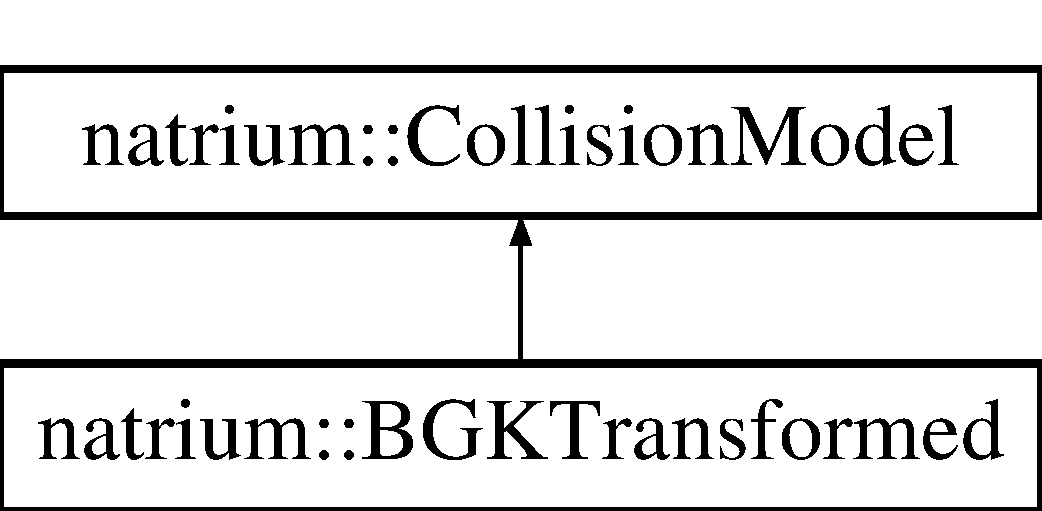
\includegraphics[height=2.000000cm]{classnatrium_1_1BGKTransformed}
\end{center}
\end{figure}
\subsection*{Public Member Functions}
\begin{DoxyCompactItemize}
\item 
\hyperlink{classnatrium_1_1BGKTransformed_aafd0ed5b888da93e496c0a29e092bf5b}{B\-G\-K\-Transformed} (double relaxation\-Parameter, boost\-::shared\-\_\-ptr$<$ \hyperlink{classnatrium_1_1BoltzmannModel}{Boltzmann\-Model} $>$ boltzmann\-Model)
\begin{DoxyCompactList}\small\item\em constructor \end{DoxyCompactList}\item 
\hypertarget{classnatrium_1_1BGKTransformed_a554c68facfbd2b126f24504f215eb193}{virtual \hyperlink{classnatrium_1_1BGKTransformed_a554c68facfbd2b126f24504f215eb193}{$\sim$\-B\-G\-K\-Transformed} ()}\label{classnatrium_1_1BGKTransformed_a554c68facfbd2b126f24504f215eb193}

\begin{DoxyCompactList}\small\item\em destructor \end{DoxyCompactList}\item 
virtual void \hyperlink{classnatrium_1_1BGKTransformed_a2e40159e5f5204431b1acb84b15910c0}{collide\-Single\-Point} (vector$<$ double $>$ \&distributions) const 
\begin{DoxyCompactList}\small\item\em function for collision \end{DoxyCompactList}\item 
virtual void \hyperlink{classnatrium_1_1BGKTransformed_a6bb41acd37234d2f92a9d868ff2486e1}{collide\-Single\-Do\-F} (size\-\_\-t do\-F, const vector$<$ double $>$ \&feq, \hyperlink{classnatrium_1_1DistributionFunctions}{Distribution\-Functions} \&f) const 
\begin{DoxyCompactList}\small\item\em virtual function for collision \end{DoxyCompactList}\end{DoxyCompactItemize}
\subsection*{Additional Inherited Members}


\subsection{Detailed Description}
Description of the B\-G\-K model for the transformed particle distributions, as described in Global data which is used by Min and Lee (2011)\-: A spectral-\/element discontinuous Galerkin lattice Boltzmann method for nearly incompressible flows, J\-C\-P 230 pp. 245-\/259. 

\subsection{Constructor \& Destructor Documentation}
\hypertarget{classnatrium_1_1BGKTransformed_aafd0ed5b888da93e496c0a29e092bf5b}{\index{natrium\-::\-B\-G\-K\-Transformed@{natrium\-::\-B\-G\-K\-Transformed}!B\-G\-K\-Transformed@{B\-G\-K\-Transformed}}
\index{B\-G\-K\-Transformed@{B\-G\-K\-Transformed}!natrium::BGKTransformed@{natrium\-::\-B\-G\-K\-Transformed}}
\subsubsection[{B\-G\-K\-Transformed}]{\setlength{\rightskip}{0pt plus 5cm}natrium\-::\-B\-G\-K\-Transformed\-::\-B\-G\-K\-Transformed (
\begin{DoxyParamCaption}
\item[{double}]{relaxation\-Parameter, }
\item[{boost\-::shared\-\_\-ptr$<$ {\bf Boltzmann\-Model} $>$}]{boltzmann\-Model}
\end{DoxyParamCaption}
)}}\label{classnatrium_1_1BGKTransformed_aafd0ed5b888da93e496c0a29e092bf5b}


constructor 


\begin{DoxyParams}[1]{Parameters}
\mbox{\tt in}  & {\em relaxation\-Parameter} & relaxation parameter tau \\
\hline
\end{DoxyParams}


\subsection{Member Function Documentation}
\hypertarget{classnatrium_1_1BGKTransformed_a6bb41acd37234d2f92a9d868ff2486e1}{\index{natrium\-::\-B\-G\-K\-Transformed@{natrium\-::\-B\-G\-K\-Transformed}!collide\-Single\-Do\-F@{collide\-Single\-Do\-F}}
\index{collide\-Single\-Do\-F@{collide\-Single\-Do\-F}!natrium::BGKTransformed@{natrium\-::\-B\-G\-K\-Transformed}}
\subsubsection[{collide\-Single\-Do\-F}]{\setlength{\rightskip}{0pt plus 5cm}void natrium\-::\-B\-G\-K\-Transformed\-::collide\-Single\-Do\-F (
\begin{DoxyParamCaption}
\item[{size\-\_\-t}]{do\-F, }
\item[{const vector$<$ double $>$ \&}]{feq, }
\item[{{\bf Distribution\-Functions} \&}]{f}
\end{DoxyParamCaption}
) const\hspace{0.3cm}{\ttfamily [virtual]}}}\label{classnatrium_1_1BGKTransformed_a6bb41acd37234d2f92a9d868ff2486e1}


virtual function for collision 


\begin{DoxyParams}[1]{Parameters}
\mbox{\tt in}  & {\em do\-F} & the do\-F index for which collision is done \\
\hline
\mbox{\tt in}  & {\em feq} & the vector of local equilibrium distributions \\
\hline
\mbox{\tt in}  & {\em f} & the vector of global distribution functions \\
\hline
\end{DoxyParams}


Implements \hyperlink{classnatrium_1_1CollisionModel_abe4f58658074680b679db7b7fddd6113}{natrium\-::\-Collision\-Model}.

\hypertarget{classnatrium_1_1BGKTransformed_a2e40159e5f5204431b1acb84b15910c0}{\index{natrium\-::\-B\-G\-K\-Transformed@{natrium\-::\-B\-G\-K\-Transformed}!collide\-Single\-Point@{collide\-Single\-Point}}
\index{collide\-Single\-Point@{collide\-Single\-Point}!natrium::BGKTransformed@{natrium\-::\-B\-G\-K\-Transformed}}
\subsubsection[{collide\-Single\-Point}]{\setlength{\rightskip}{0pt plus 5cm}void natrium\-::\-B\-G\-K\-Transformed\-::collide\-Single\-Point (
\begin{DoxyParamCaption}
\item[{vector$<$ double $>$ \&}]{distributions}
\end{DoxyParamCaption}
) const\hspace{0.3cm}{\ttfamily [virtual]}}}\label{classnatrium_1_1BGKTransformed_a2e40159e5f5204431b1acb84b15910c0}


function for collision 


\begin{DoxyParams}{Parameters}
{\em in/out\mbox{]}} & distributions the particle distribution functions \\
\hline
\end{DoxyParams}


Implements \hyperlink{classnatrium_1_1CollisionModel_acde767e924eb2124ab3eb725543111e8}{natrium\-::\-Collision\-Model}.



The documentation for this class was generated from the following files\-:\begin{DoxyCompactItemize}
\item 
/home/kraemer/eclipse\-\_\-workspace/\-N\-A\-Triu\-M/src/natrium/collisionmodels/\hyperlink{BGKTransformed_8h}{B\-G\-K\-Transformed.\-h}\item 
/home/kraemer/eclipse\-\_\-workspace/\-N\-A\-Triu\-M/src/natrium/collisionmodels/\hyperlink{BGKTransformed_8cpp}{B\-G\-K\-Transformed.\-cpp}\end{DoxyCompactItemize}

\hypertarget{classnatrium_1_1BoltzmannModel}{\section{natrium\-:\-:\-Boltzmann\-Model \-Class \-Reference}
\label{classnatrium_1_1BoltzmannModel}\index{natrium\-::\-Boltzmann\-Model@{natrium\-::\-Boltzmann\-Model}}
}


\-Abstract class for the description of a boltzmann model, e.\-g. \-D2\-Q9.  




{\ttfamily \#include $<$\-Boltzmann\-Model.\-h$>$}

\-Inheritance diagram for natrium\-:\-:\-Boltzmann\-Model\-:\begin{figure}[H]
\begin{center}
\leavevmode
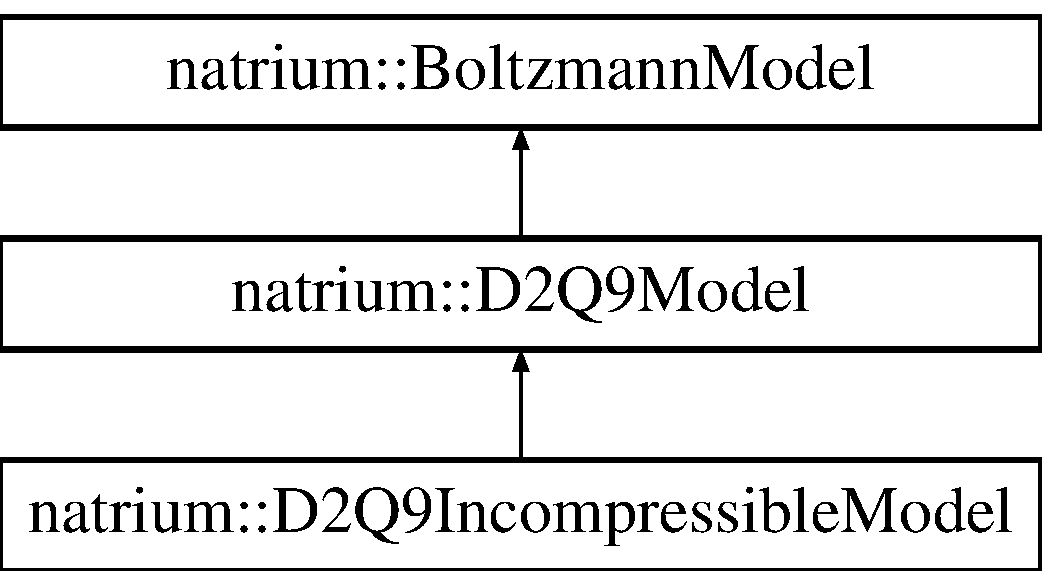
\includegraphics[height=3.000000cm]{classnatrium_1_1BoltzmannModel}
\end{center}
\end{figure}
\subsection*{\-Public \-Member \-Functions}
\begin{DoxyCompactItemize}
\item 
\hyperlink{classnatrium_1_1BoltzmannModel_a0547ee3c88330d7a2ac44ad3ece8d560}{\-Boltzmann\-Model} (size\-\_\-t d, size\-\_\-t q, const vector$<$ numeric\-\_\-vector $>$ \&directions, const vector$<$ float\-\_\-t $>$ \&weights, \-Stencil\-Type stencil\-Type)
\begin{DoxyCompactList}\small\item\em constructor \end{DoxyCompactList}\item 
\hypertarget{classnatrium_1_1BoltzmannModel_ac2e3dabcbe15c1e37ff09ec1c53dafa5}{virtual \hyperlink{classnatrium_1_1BoltzmannModel_ac2e3dabcbe15c1e37ff09ec1c53dafa5}{$\sim$\-Boltzmann\-Model} ()}\label{classnatrium_1_1BoltzmannModel_ac2e3dabcbe15c1e37ff09ec1c53dafa5}

\begin{DoxyCompactList}\small\item\em destructor \end{DoxyCompactList}\item 
const vector$<$ numeric\-\_\-vector $>$ \& \hyperlink{classnatrium_1_1BoltzmannModel_aeabed4142acd04a57ba41ca26dfbe666}{get\-Directions} () const 
\begin{DoxyCompactList}\small\item\em get a reference to the vector of directions \end{DoxyCompactList}\item 
const numeric\-\_\-vector \& \hyperlink{classnatrium_1_1BoltzmannModel_a0b258b2c7cc4cba5ac666a06ca2a8f49}{get\-Direction} (size\-\_\-t i) const 
\begin{DoxyCompactList}\small\item\em get the i-\/th direction \end{DoxyCompactList}\item 
size\-\_\-t \hyperlink{classnatrium_1_1BoltzmannModel_ae7cfcd108a085d3215cdc8c00e826107}{get\-Q} () const 
\begin{DoxyCompactList}\small\item\em get q, the number of directions in the \-Dd\-Qq-\/stencil \end{DoxyCompactList}\item 
size\-\_\-t \hyperlink{classnatrium_1_1BoltzmannModel_a8d16745a0dab65cb0324d6b076e53d15}{get\-D} () const 
\begin{DoxyCompactList}\small\item\em get d, the dimension of the \-Dd\-Qq-\/stencil \end{DoxyCompactList}\item 
const vector$<$ float\-\_\-t $>$ \& \hyperlink{classnatrium_1_1BoltzmannModel_a3158e70071707c169486d87d26727f3c}{get\-Weights} () const 
\begin{DoxyCompactList}\small\item\em get the weights of the equilibrium distributions \end{DoxyCompactList}\item 
float\-\_\-t \hyperlink{classnatrium_1_1BoltzmannModel_aae549c1f5dd48a92fc9e174afc5de1a5}{get\-Weight} (size\-\_\-t i) const 
\begin{DoxyCompactList}\small\item\em get the weight belonging to a certain direction \end{DoxyCompactList}\item 
const \-Stencil\-Type \hyperlink{classnatrium_1_1BoltzmannModel_ac95c2547a37e380d8d7b3de3c0f8a4c2}{get\-Stencil\-Type} () const 
\begin{DoxyCompactList}\small\item\em get stencil type \end{DoxyCompactList}\item 
float\-\_\-t \hyperlink{classnatrium_1_1BoltzmannModel_adf8901da899eef5d11b0cbf80200ee32}{calculate\-Density} (const vector$<$ float\-\_\-t $>$ \&distributions) const 
\begin{DoxyCompactList}\small\item\em calculate macroscopic density \end{DoxyCompactList}\item 
numeric\-\_\-vector \hyperlink{classnatrium_1_1BoltzmannModel_a2c7e3465bb3541e420f15a7970533047}{calculate\-Velocity} (const vector$<$ float\-\_\-t $>$ \&distributions) const 
\begin{DoxyCompactList}\small\item\em calculate macroscopic velocity \end{DoxyCompactList}\item 
void \hyperlink{classnatrium_1_1BoltzmannModel_a3d5a504ad3dc0b3847c5db412b1988b8}{calculate\-Velocity} (const vector$<$ float\-\_\-t $>$ \&distributions, const float\-\_\-t rho, numeric\-\_\-vector \&u) const 
\begin{DoxyCompactList}\small\item\em calculate macroscopic velocity; saves the double calculation of the density \end{DoxyCompactList}\item 
virtual float\-\_\-t \hyperlink{classnatrium_1_1BoltzmannModel_ac5615f43cd5c03c881734d4826ce31be}{get\-Equilibrium\-Distribution} (size\-\_\-t i, const numeric\-\_\-vector \&u, const float\-\_\-t rho=1) const =0
\begin{DoxyCompactList}\small\item\em virtual function for the calculation of the equilibrium distribution \end{DoxyCompactList}\item 
virtual void \hyperlink{classnatrium_1_1BoltzmannModel_aab8d824211e65a394536333c5537b325}{get\-Equilibrium\-Distributions} (vector$<$ float\-\_\-t $>$ \&feq, const numeric\-\_\-vector \&u, const float\-\_\-t rho=1) const 
\begin{DoxyCompactList}\small\item\em function for the calculation of all equilibrium distributions \end{DoxyCompactList}\end{DoxyCompactItemize}


\subsection{\-Detailed \-Description}
\-Abstract class for the description of a boltzmann model, e.\-g. \-D2\-Q9. 

\subsection{\-Constructor \& \-Destructor \-Documentation}
\hypertarget{classnatrium_1_1BoltzmannModel_a0547ee3c88330d7a2ac44ad3ece8d560}{\index{natrium\-::\-Boltzmann\-Model@{natrium\-::\-Boltzmann\-Model}!\-Boltzmann\-Model@{\-Boltzmann\-Model}}
\index{\-Boltzmann\-Model@{\-Boltzmann\-Model}!natrium::BoltzmannModel@{natrium\-::\-Boltzmann\-Model}}
\subsubsection[{\-Boltzmann\-Model}]{\setlength{\rightskip}{0pt plus 5cm}{\bf natrium\-::\-Boltzmann\-Model\-::\-Boltzmann\-Model} (
\begin{DoxyParamCaption}
\item[{size\-\_\-t}]{d, }
\item[{size\-\_\-t}]{q, }
\item[{const vector$<$ numeric\-\_\-vector $>$ \&}]{directions, }
\item[{const vector$<$ float\-\_\-t $>$ \&}]{weights, }
\item[{\-Stencil\-Type}]{stencil\-Type}
\end{DoxyParamCaption}
)}}\label{classnatrium_1_1BoltzmannModel_a0547ee3c88330d7a2ac44ad3ece8d560}


constructor 


\begin{DoxyParams}{\-Parameters}
{\em d} & dimension \\
\hline
{\em q} & number of directions \\
\hline
{\em directions} & the directions of the stencil \\
\hline
{\em weights} & the weights of the equilibrium distribution \\
\hline
{\em stencil\-Type} & type of the stencil (e.\-g. \-D2\-Q9) \\
\hline
\end{DoxyParams}


\subsection{\-Member \-Function \-Documentation}
\hypertarget{classnatrium_1_1BoltzmannModel_adf8901da899eef5d11b0cbf80200ee32}{\index{natrium\-::\-Boltzmann\-Model@{natrium\-::\-Boltzmann\-Model}!calculate\-Density@{calculate\-Density}}
\index{calculate\-Density@{calculate\-Density}!natrium::BoltzmannModel@{natrium\-::\-Boltzmann\-Model}}
\subsubsection[{calculate\-Density}]{\setlength{\rightskip}{0pt plus 5cm}float\-\_\-t {\bf natrium\-::\-Boltzmann\-Model\-::calculate\-Density} (
\begin{DoxyParamCaption}
\item[{const vector$<$ float\-\_\-t $>$ \&}]{distributions}
\end{DoxyParamCaption}
) const\hspace{0.3cm}{\ttfamily  \mbox{[}inline\mbox{]}}}}\label{classnatrium_1_1BoltzmannModel_adf8901da899eef5d11b0cbf80200ee32}


calculate macroscopic density 


\begin{DoxyParams}[1]{\-Parameters}
\mbox{\tt in}  & {\em distributions} & particle distribution functions at a given point \\
\hline
\end{DoxyParams}
\begin{DoxyReturn}{\-Returns}
macroscopic density (sum of all distributions) 
\end{DoxyReturn}
\hypertarget{classnatrium_1_1BoltzmannModel_a2c7e3465bb3541e420f15a7970533047}{\index{natrium\-::\-Boltzmann\-Model@{natrium\-::\-Boltzmann\-Model}!calculate\-Velocity@{calculate\-Velocity}}
\index{calculate\-Velocity@{calculate\-Velocity}!natrium::BoltzmannModel@{natrium\-::\-Boltzmann\-Model}}
\subsubsection[{calculate\-Velocity}]{\setlength{\rightskip}{0pt plus 5cm}numeric\-\_\-vector {\bf natrium\-::\-Boltzmann\-Model\-::calculate\-Velocity} (
\begin{DoxyParamCaption}
\item[{const vector$<$ float\-\_\-t $>$ \&}]{distributions}
\end{DoxyParamCaption}
) const\hspace{0.3cm}{\ttfamily  \mbox{[}inline\mbox{]}}}}\label{classnatrium_1_1BoltzmannModel_a2c7e3465bb3541e420f15a7970533047}


calculate macroscopic velocity 


\begin{DoxyParams}[1]{\-Parameters}
\mbox{\tt in}  & {\em distributions} & particle distribution functions at a given point \\
\hline
\end{DoxyParams}
\begin{DoxyReturn}{\-Returns}
macroscopic velocity 
\end{DoxyReturn}
\hypertarget{classnatrium_1_1BoltzmannModel_a3d5a504ad3dc0b3847c5db412b1988b8}{\index{natrium\-::\-Boltzmann\-Model@{natrium\-::\-Boltzmann\-Model}!calculate\-Velocity@{calculate\-Velocity}}
\index{calculate\-Velocity@{calculate\-Velocity}!natrium::BoltzmannModel@{natrium\-::\-Boltzmann\-Model}}
\subsubsection[{calculate\-Velocity}]{\setlength{\rightskip}{0pt plus 5cm}void {\bf natrium\-::\-Boltzmann\-Model\-::calculate\-Velocity} (
\begin{DoxyParamCaption}
\item[{const vector$<$ float\-\_\-t $>$ \&}]{distributions, }
\item[{const float\-\_\-t}]{rho, }
\item[{numeric\-\_\-vector \&}]{u}
\end{DoxyParamCaption}
) const\hspace{0.3cm}{\ttfamily  \mbox{[}inline\mbox{]}}}}\label{classnatrium_1_1BoltzmannModel_a3d5a504ad3dc0b3847c5db412b1988b8}


calculate macroscopic velocity; saves the double calculation of the density 

\begin{DoxyNote}{\-Note}
more efficient 
\end{DoxyNote}

\begin{DoxyParams}[1]{\-Parameters}
\mbox{\tt in}  & {\em distributions} & particle distribution functions at a given point \\
\hline
\mbox{\tt in}  & {\em rho} & macroscopic density \\
\hline
\mbox{\tt out}  & {\em u} & macroscopic velocity \\
\hline
\end{DoxyParams}
\hypertarget{classnatrium_1_1BoltzmannModel_a8d16745a0dab65cb0324d6b076e53d15}{\index{natrium\-::\-Boltzmann\-Model@{natrium\-::\-Boltzmann\-Model}!get\-D@{get\-D}}
\index{get\-D@{get\-D}!natrium::BoltzmannModel@{natrium\-::\-Boltzmann\-Model}}
\subsubsection[{get\-D}]{\setlength{\rightskip}{0pt plus 5cm}size\-\_\-t {\bf natrium\-::\-Boltzmann\-Model\-::get\-D} (
\begin{DoxyParamCaption}
{}
\end{DoxyParamCaption}
) const\hspace{0.3cm}{\ttfamily  \mbox{[}inline\mbox{]}}}}\label{classnatrium_1_1BoltzmannModel_a8d16745a0dab65cb0324d6b076e53d15}


get d, the dimension of the \-Dd\-Qq-\/stencil 

\begin{DoxyReturn}{\-Returns}
d 
\end{DoxyReturn}
\hypertarget{classnatrium_1_1BoltzmannModel_a0b258b2c7cc4cba5ac666a06ca2a8f49}{\index{natrium\-::\-Boltzmann\-Model@{natrium\-::\-Boltzmann\-Model}!get\-Direction@{get\-Direction}}
\index{get\-Direction@{get\-Direction}!natrium::BoltzmannModel@{natrium\-::\-Boltzmann\-Model}}
\subsubsection[{get\-Direction}]{\setlength{\rightskip}{0pt plus 5cm}const numeric\-\_\-vector\& {\bf natrium\-::\-Boltzmann\-Model\-::get\-Direction} (
\begin{DoxyParamCaption}
\item[{size\-\_\-t}]{i}
\end{DoxyParamCaption}
) const\hspace{0.3cm}{\ttfamily  \mbox{[}inline\mbox{]}}}}\label{classnatrium_1_1BoltzmannModel_a0b258b2c7cc4cba5ac666a06ca2a8f49}


get the i-\/th direction 


\begin{DoxyParams}{\-Parameters}
{\em i} & index i \\
\hline
\end{DoxyParams}
\begin{DoxyReturn}{\-Returns}
a reference to the i-\/th direction of the \-Dd\-Qq-\/stencil 
\end{DoxyReturn}
\hypertarget{classnatrium_1_1BoltzmannModel_aeabed4142acd04a57ba41ca26dfbe666}{\index{natrium\-::\-Boltzmann\-Model@{natrium\-::\-Boltzmann\-Model}!get\-Directions@{get\-Directions}}
\index{get\-Directions@{get\-Directions}!natrium::BoltzmannModel@{natrium\-::\-Boltzmann\-Model}}
\subsubsection[{get\-Directions}]{\setlength{\rightskip}{0pt plus 5cm}const vector$<$numeric\-\_\-vector$>$\& {\bf natrium\-::\-Boltzmann\-Model\-::get\-Directions} (
\begin{DoxyParamCaption}
{}
\end{DoxyParamCaption}
) const\hspace{0.3cm}{\ttfamily  \mbox{[}inline\mbox{]}}}}\label{classnatrium_1_1BoltzmannModel_aeabed4142acd04a57ba41ca26dfbe666}


get a reference to the vector of directions 

\begin{DoxyReturn}{\-Returns}
a ublas\-\_\-vector, which contains the directions of the \-Dd\-Qq-\/stencil as ublas\-\_\-vectors 
\end{DoxyReturn}
\hypertarget{classnatrium_1_1BoltzmannModel_ac5615f43cd5c03c881734d4826ce31be}{\index{natrium\-::\-Boltzmann\-Model@{natrium\-::\-Boltzmann\-Model}!get\-Equilibrium\-Distribution@{get\-Equilibrium\-Distribution}}
\index{get\-Equilibrium\-Distribution@{get\-Equilibrium\-Distribution}!natrium::BoltzmannModel@{natrium\-::\-Boltzmann\-Model}}
\subsubsection[{get\-Equilibrium\-Distribution}]{\setlength{\rightskip}{0pt plus 5cm}virtual float\-\_\-t {\bf natrium\-::\-Boltzmann\-Model\-::get\-Equilibrium\-Distribution} (
\begin{DoxyParamCaption}
\item[{size\-\_\-t}]{i, }
\item[{const numeric\-\_\-vector \&}]{u, }
\item[{const float\-\_\-t}]{rho = {\ttfamily 1}}
\end{DoxyParamCaption}
) const\hspace{0.3cm}{\ttfamily  \mbox{[}pure virtual\mbox{]}}}}\label{classnatrium_1_1BoltzmannModel_ac5615f43cd5c03c881734d4826ce31be}


virtual function for the calculation of the equilibrium distribution 


\begin{DoxyParams}{\-Parameters}
{\em i} & index of the direction \\
\hline
{\em u} & macroscopic velocity \\
\hline
{\em rho} & macroscopic density \\
\hline
\end{DoxyParams}
\begin{DoxyReturn}{\-Returns}
value of the equilibrium distribution 
\end{DoxyReturn}
\begin{DoxyNote}{\-Note}
\-The calculation can surely be done more efficiently by passing different arguments, e.\-g. u$\ast$u or u/(c$^\wedge$2) 
\end{DoxyNote}


\-Implemented in \hyperlink{classnatrium_1_1D2Q9IncompressibleModel_a437bce6e0d6f35ca3ff2df4bbe650043}{natrium\-::\-D2\-Q9\-Incompressible\-Model}.

\hypertarget{classnatrium_1_1BoltzmannModel_aab8d824211e65a394536333c5537b325}{\index{natrium\-::\-Boltzmann\-Model@{natrium\-::\-Boltzmann\-Model}!get\-Equilibrium\-Distributions@{get\-Equilibrium\-Distributions}}
\index{get\-Equilibrium\-Distributions@{get\-Equilibrium\-Distributions}!natrium::BoltzmannModel@{natrium\-::\-Boltzmann\-Model}}
\subsubsection[{get\-Equilibrium\-Distributions}]{\setlength{\rightskip}{0pt plus 5cm}void {\bf natrium\-::\-Boltzmann\-Model\-::get\-Equilibrium\-Distributions} (
\begin{DoxyParamCaption}
\item[{vector$<$ float\-\_\-t $>$ \&}]{feq, }
\item[{const numeric\-\_\-vector \&}]{u, }
\item[{const float\-\_\-t}]{rho = {\ttfamily 1}}
\end{DoxyParamCaption}
) const\hspace{0.3cm}{\ttfamily  \mbox{[}virtual\mbox{]}}}}\label{classnatrium_1_1BoltzmannModel_aab8d824211e65a394536333c5537b325}


function for the calculation of all equilibrium distributions 


\begin{DoxyParams}[1]{\-Parameters}
\mbox{\tt out}  & {\em feq} & vector of all equality distributions, must have size \-Q \\
\hline
\mbox{\tt in}  & {\em u} & macroscopic velocity \\
\hline
\mbox{\tt in}  & {\em rho} & macroscopic density \\
\hline
\end{DoxyParams}
\begin{DoxyNote}{\-Note}
\-The calculation can surely be done more efficiently by passing different arguments, e.\-g. u$\ast$u or u/(c$^\wedge$2) 
\end{DoxyNote}
\hypertarget{classnatrium_1_1BoltzmannModel_ae7cfcd108a085d3215cdc8c00e826107}{\index{natrium\-::\-Boltzmann\-Model@{natrium\-::\-Boltzmann\-Model}!get\-Q@{get\-Q}}
\index{get\-Q@{get\-Q}!natrium::BoltzmannModel@{natrium\-::\-Boltzmann\-Model}}
\subsubsection[{get\-Q}]{\setlength{\rightskip}{0pt plus 5cm}size\-\_\-t {\bf natrium\-::\-Boltzmann\-Model\-::get\-Q} (
\begin{DoxyParamCaption}
{}
\end{DoxyParamCaption}
) const\hspace{0.3cm}{\ttfamily  \mbox{[}inline\mbox{]}}}}\label{classnatrium_1_1BoltzmannModel_ae7cfcd108a085d3215cdc8c00e826107}


get q, the number of directions in the \-Dd\-Qq-\/stencil 

\begin{DoxyReturn}{\-Returns}
q 
\end{DoxyReturn}
\hypertarget{classnatrium_1_1BoltzmannModel_ac95c2547a37e380d8d7b3de3c0f8a4c2}{\index{natrium\-::\-Boltzmann\-Model@{natrium\-::\-Boltzmann\-Model}!get\-Stencil\-Type@{get\-Stencil\-Type}}
\index{get\-Stencil\-Type@{get\-Stencil\-Type}!natrium::BoltzmannModel@{natrium\-::\-Boltzmann\-Model}}
\subsubsection[{get\-Stencil\-Type}]{\setlength{\rightskip}{0pt plus 5cm}const \-Stencil\-Type {\bf natrium\-::\-Boltzmann\-Model\-::get\-Stencil\-Type} (
\begin{DoxyParamCaption}
{}
\end{DoxyParamCaption}
) const\hspace{0.3cm}{\ttfamily  \mbox{[}inline\mbox{]}}}}\label{classnatrium_1_1BoltzmannModel_ac95c2547a37e380d8d7b3de3c0f8a4c2}


get stencil type 

\begin{DoxyReturn}{\-Returns}
stencil type, e.\-g. \-D2\-Q9 
\end{DoxyReturn}
\hypertarget{classnatrium_1_1BoltzmannModel_aae549c1f5dd48a92fc9e174afc5de1a5}{\index{natrium\-::\-Boltzmann\-Model@{natrium\-::\-Boltzmann\-Model}!get\-Weight@{get\-Weight}}
\index{get\-Weight@{get\-Weight}!natrium::BoltzmannModel@{natrium\-::\-Boltzmann\-Model}}
\subsubsection[{get\-Weight}]{\setlength{\rightskip}{0pt plus 5cm}float\-\_\-t {\bf natrium\-::\-Boltzmann\-Model\-::get\-Weight} (
\begin{DoxyParamCaption}
\item[{size\-\_\-t}]{i}
\end{DoxyParamCaption}
) const\hspace{0.3cm}{\ttfamily  \mbox{[}inline\mbox{]}}}}\label{classnatrium_1_1BoltzmannModel_aae549c1f5dd48a92fc9e174afc5de1a5}


get the weight belonging to a certain direction 


\begin{DoxyParams}{\-Parameters}
{\em i} & index i of the direction (1 $<$= i $<$= q) \\
\hline
\end{DoxyParams}
\begin{DoxyReturn}{\-Returns}
the i-\/th weight 
\end{DoxyReturn}
\hypertarget{classnatrium_1_1BoltzmannModel_a3158e70071707c169486d87d26727f3c}{\index{natrium\-::\-Boltzmann\-Model@{natrium\-::\-Boltzmann\-Model}!get\-Weights@{get\-Weights}}
\index{get\-Weights@{get\-Weights}!natrium::BoltzmannModel@{natrium\-::\-Boltzmann\-Model}}
\subsubsection[{get\-Weights}]{\setlength{\rightskip}{0pt plus 5cm}const vector$<$float\-\_\-t$>$\& {\bf natrium\-::\-Boltzmann\-Model\-::get\-Weights} (
\begin{DoxyParamCaption}
{}
\end{DoxyParamCaption}
) const\hspace{0.3cm}{\ttfamily  \mbox{[}inline\mbox{]}}}}\label{classnatrium_1_1BoltzmannModel_a3158e70071707c169486d87d26727f3c}


get the weights of the equilibrium distributions 

\begin{DoxyReturn}{\-Returns}
a reference to the vector of weights 
\end{DoxyReturn}


\-The documentation for this class was generated from the following files\-:\begin{DoxyCompactItemize}
\item 
/home/kraemer/eclipse\-\_\-workspace/\-N\-A\-Triu\-M/src/boltzmannmodels/\hyperlink{BoltzmannModel_8h}{\-Boltzmann\-Model.\-h}\item 
/home/kraemer/eclipse\-\_\-workspace/\-N\-A\-Triu\-M/src/boltzmannmodels/\hyperlink{BoltzmannModel_8cpp}{\-Boltzmann\-Model.\-cpp}\end{DoxyCompactItemize}

\hypertarget{classnatrium_1_1CFDSolver}{
\section{natrium::CFDSolver$<$ dim $>$ Class Template Reference}
\label{classnatrium_1_1CFDSolver}\index{natrium::CFDSolver@{natrium::CFDSolver}}
}


The central class for the CFD simulation based on the DBE.  


{\ttfamily \#include $<$CFDSolver.h$>$}Inheritance diagram for natrium::CFDSolver$<$ dim $>$::\begin{figure}[H]
\begin{center}
\leavevmode
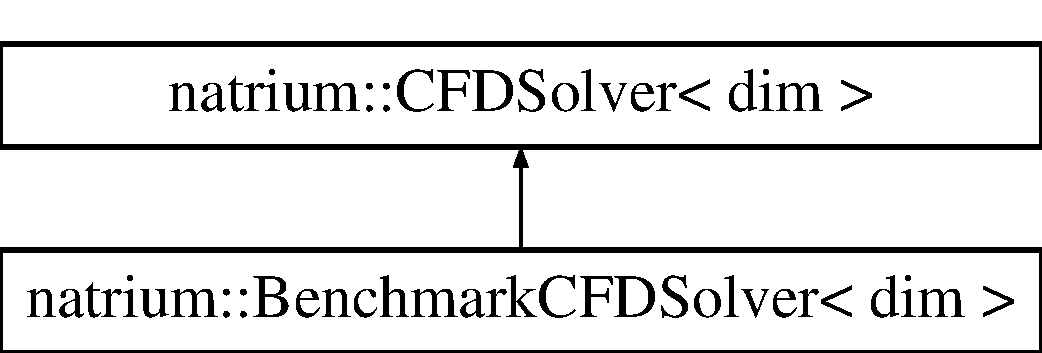
\includegraphics[height=2cm]{classnatrium_1_1CFDSolver}
\end{center}
\end{figure}
\subsection*{Public Member Functions}
\begin{DoxyCompactItemize}
\item 
\hyperlink{classnatrium_1_1CFDSolver_a9d0e65b8a404ac3eaf80aee6c81945dc}{CFDSolver} (shared\_\-ptr$<$ \hyperlink{classnatrium_1_1SolverConfiguration}{SolverConfiguration} $>$ configuration, shared\_\-ptr$<$ \hyperlink{classnatrium_1_1ProblemDescription}{ProblemDescription}$<$ dim $>$ $>$ problemDescription)
\item 
\hypertarget{classnatrium_1_1CFDSolver_a7ca9bd709255ac87b34f869c984b913b}{
virtual \hyperlink{classnatrium_1_1CFDSolver_a7ca9bd709255ac87b34f869c984b913b}{$\sim$CFDSolver} ()}
\label{classnatrium_1_1CFDSolver_a7ca9bd709255ac87b34f869c984b913b}

\begin{DoxyCompactList}\small\item\em destructor \item\end{DoxyCompactList}\item 
\hypertarget{classnatrium_1_1CFDSolver_abe627b0bbde0635abb30b9bea4c72dc1}{
void \hyperlink{classnatrium_1_1CFDSolver_abe627b0bbde0635abb30b9bea4c72dc1}{initializeDistributions} ()}
\label{classnatrium_1_1CFDSolver_abe627b0bbde0635abb30b9bea4c72dc1}

\begin{DoxyCompactList}\small\item\em initialize distribution functions \item\end{DoxyCompactList}\item 
\hypertarget{classnatrium_1_1CFDSolver_ac32a318e504b31195eb61c2cdc2659fe}{
void \hyperlink{classnatrium_1_1CFDSolver_ac32a318e504b31195eb61c2cdc2659fe}{stream} ()}
\label{classnatrium_1_1CFDSolver_ac32a318e504b31195eb61c2cdc2659fe}

\begin{DoxyCompactList}\small\item\em Advection in all directions. \item\end{DoxyCompactList}\item 
\hypertarget{classnatrium_1_1CFDSolver_ac9bec7d0c4bcd5e02c5213ec09438c02}{
void \hyperlink{classnatrium_1_1CFDSolver_ac9bec7d0c4bcd5e02c5213ec09438c02}{collide} ()}
\label{classnatrium_1_1CFDSolver_ac9bec7d0c4bcd5e02c5213ec09438c02}

\begin{DoxyCompactList}\small\item\em Low-\/level collide function. \item\end{DoxyCompactList}\item 
\hypertarget{classnatrium_1_1CFDSolver_a604212a1f6cd2549b8f60ab26b14de00}{
void \hyperlink{classnatrium_1_1CFDSolver_a604212a1f6cd2549b8f60ab26b14de00}{reassemble} ()}
\label{classnatrium_1_1CFDSolver_a604212a1f6cd2549b8f60ab26b14de00}

\begin{DoxyCompactList}\small\item\em reassembly of all matrices \item\end{DoxyCompactList}\item 
\hypertarget{classnatrium_1_1CFDSolver_a11f503bc3f3c306b240874c74a38025b}{
void \hyperlink{classnatrium_1_1CFDSolver_a11f503bc3f3c306b240874c74a38025b}{run} ()}
\label{classnatrium_1_1CFDSolver_a11f503bc3f3c306b240874c74a38025b}

\begin{DoxyCompactList}\small\item\em run CFD solver \item\end{DoxyCompactList}\item 
\hypertarget{classnatrium_1_1CFDSolver_a9a144e7e757e1b1c26f32b712b17c70e}{
bool \hyperlink{classnatrium_1_1CFDSolver_a9a144e7e757e1b1c26f32b712b17c70e}{stopConditionMet} ()}
\label{classnatrium_1_1CFDSolver_a9a144e7e757e1b1c26f32b712b17c70e}

\begin{DoxyCompactList}\small\item\em test for stop conditions \item\end{DoxyCompactList}\item 
void \hyperlink{classnatrium_1_1CFDSolver_a36146c0f8a6c5abd0ebec4c49f2a4e6d}{applyInitialDensities} (distributed\_\-vector \&initialDensities, const map$<$ dealii::types::global\_\-dof\_\-index, dealii::Point$<$ dim $>$ $>$ \&supportPoints) const 
\begin{DoxyCompactList}\small\item\em set initial densities \item\end{DoxyCompactList}\item 
void \hyperlink{classnatrium_1_1CFDSolver_afd82bfa5e1e613ef99b9b870cb73db0e}{applyInitialVelocities} (vector$<$ distributed\_\-vector $>$ \&initialVelocities, const map$<$ dealii::types::global\_\-dof\_\-index, dealii::Point$<$ dim $>$ $>$ \&supportPoints) const 
\begin{DoxyCompactList}\small\item\em set initial velocities \item\end{DoxyCompactList}\item 
virtual void \hyperlink{classnatrium_1_1CFDSolver_abf6804f132885502b61877fc1f9ca4a2}{output} (size\_\-t iteration)
\begin{DoxyCompactList}\small\item\em create output data and write to file \item\end{DoxyCompactList}\item 
\hypertarget{classnatrium_1_1CFDSolver_a9c3f844b4c6b670aac83bc3ad5519fad}{
bool {\bfseries hasGeometryChanged} ()}
\label{classnatrium_1_1CFDSolver_a9c3f844b4c6b670aac83bc3ad5519fad}

\item 
\hypertarget{classnatrium_1_1CFDSolver_adf0b4e4da292bcb195d926d3174ba2a9}{
const distributed\_\-vector \& {\bfseries getDensity} () const }
\label{classnatrium_1_1CFDSolver_adf0b4e4da292bcb195d926d3174ba2a9}

\item 
\hypertarget{classnatrium_1_1CFDSolver_a963e069873d88d130b0fe3f7f77c3d83}{
const \hyperlink{classnatrium_1_1DistributionFunctions}{DistributionFunctions} \& {\bfseries getF} () const }
\label{classnatrium_1_1CFDSolver_a963e069873d88d130b0fe3f7f77c3d83}

\item 
\hypertarget{classnatrium_1_1CFDSolver_a0e5ec3dc278216d5827410b7db82af59}{
const vector$<$ distributed\_\-vector $>$ \& {\bfseries getVelocity} () const }
\label{classnatrium_1_1CFDSolver_a0e5ec3dc278216d5827410b7db82af59}

\item 
\hypertarget{classnatrium_1_1CFDSolver_a1aea207c81089c2e46092489557bb139}{
const shared\_\-ptr$<$ \hyperlink{classnatrium_1_1AdvectionOperator}{AdvectionOperator}$<$ dim $>$ $>$ \& {\bfseries getAdvectionOperator} () const }
\label{classnatrium_1_1CFDSolver_a1aea207c81089c2e46092489557bb139}

\item 
\hypertarget{classnatrium_1_1CFDSolver_a2006f7bbbf2336789a5cd74d329c2e60}{
const shared\_\-ptr$<$ \hyperlink{classnatrium_1_1Stencil}{Stencil} $>$ \& {\bfseries getStencil} () const }
\label{classnatrium_1_1CFDSolver_a2006f7bbbf2336789a5cd74d329c2e60}

\item 
\hypertarget{classnatrium_1_1CFDSolver_abb4b632b524bd68afcdff7d54c2d3d97}{
const shared\_\-ptr$<$ \hyperlink{classnatrium_1_1CollisionModel}{CollisionModel} $>$ \& {\bfseries getCollisionModel} () const }
\label{classnatrium_1_1CFDSolver_abb4b632b524bd68afcdff7d54c2d3d97}

\item 
\hypertarget{classnatrium_1_1CFDSolver_a413691491ac82f384a03293be2294de5}{
const shared\_\-ptr$<$ \hyperlink{classnatrium_1_1SolverConfiguration}{SolverConfiguration} $>$ \& {\bfseries getConfiguration} () const }
\label{classnatrium_1_1CFDSolver_a413691491ac82f384a03293be2294de5}

\item 
\hypertarget{classnatrium_1_1CFDSolver_a8b1131e8fd6b022bea5ddce72469c289}{
const shared\_\-ptr$<$ \hyperlink{classnatrium_1_1ProblemDescription}{ProblemDescription}$<$ dim $>$ $>$ \& {\bfseries getProblemDescription} () const }
\label{classnatrium_1_1CFDSolver_a8b1131e8fd6b022bea5ddce72469c289}

\item 
\hypertarget{classnatrium_1_1CFDSolver_af1b1ca6771029003bc9bac7cfe0b4d3c}{
const shared\_\-ptr$<$ \hyperlink{classnatrium_1_1TimeIntegrator}{TimeIntegrator}$<$ distributed\_\-vector, distributed\_\-sparse\_\-matrix $>$ $>$ \& {\bfseries getTimeIntegrator} () const }
\label{classnatrium_1_1CFDSolver_af1b1ca6771029003bc9bac7cfe0b4d3c}

\item 
\hypertarget{classnatrium_1_1CFDSolver_a74d459ef4f43d42e04ceb2178bb006f4}{
size\_\-t {\bfseries getNumberOfDoFs} () const }
\label{classnatrium_1_1CFDSolver_a74d459ef4f43d42e04ceb2178bb006f4}

\item 
\hypertarget{classnatrium_1_1CFDSolver_ae9c44bb0f33e2c73ee96fbe100061842}{
double {\bfseries getMaxVelocityNorm} () const }
\label{classnatrium_1_1CFDSolver_ae9c44bb0f33e2c73ee96fbe100061842}

\item 
\hypertarget{classnatrium_1_1CFDSolver_ade641431988a82cb47d88a9d600e1c92}{
double {\bfseries getMaxDensityDeviationFrom} (double referenceDensity) const }
\label{classnatrium_1_1CFDSolver_ade641431988a82cb47d88a9d600e1c92}

\item 
\hypertarget{classnatrium_1_1CFDSolver_a33c4bfd63b8d457a5bc15f0c0da02c38}{
size\_\-t {\bfseries getIterationStart} () const }
\label{classnatrium_1_1CFDSolver_a33c4bfd63b8d457a5bc15f0c0da02c38}

\item 
\hypertarget{classnatrium_1_1CFDSolver_a8e3686b16794c0040bd5cc7cf9fe98d3}{
double {\bfseries getTime} () const }
\label{classnatrium_1_1CFDSolver_a8e3686b16794c0040bd5cc7cf9fe98d3}

\item 
\hypertarget{classnatrium_1_1CFDSolver_a3c0920e02df800abcfb8f82518cab0ca}{
size\_\-t {\bfseries getIteration} () const }
\label{classnatrium_1_1CFDSolver_a3c0920e02df800abcfb8f82518cab0ca}

\item 
\hypertarget{classnatrium_1_1CFDSolver_a97546801de9259206f9611c14ce9ff1d}{
void {\bfseries setIteration} (size\_\-t iteration)}
\label{classnatrium_1_1CFDSolver_a97546801de9259206f9611c14ce9ff1d}

\item 
\hypertarget{classnatrium_1_1CFDSolver_ab40725ea85fde34033d92027d13a4b06}{
const shared\_\-ptr$<$ \hyperlink{classnatrium_1_1SolverStats}{SolverStats}$<$ dim $>$ $>$ \& {\bfseries getSolverStats} () const }
\label{classnatrium_1_1CFDSolver_ab40725ea85fde34033d92027d13a4b06}

\item 
\hypertarget{classnatrium_1_1CFDSolver_abcce31d3ba9b00e148780b6c855d189b}{
double {\bfseries getTau} () const }
\label{classnatrium_1_1CFDSolver_abcce31d3ba9b00e148780b6c855d189b}

\item 
\hypertarget{classnatrium_1_1CFDSolver_a1a508263caff799245a183989efd6680}{
double {\bfseries getResiduumDensity} () const }
\label{classnatrium_1_1CFDSolver_a1a508263caff799245a183989efd6680}

\item 
\hypertarget{classnatrium_1_1CFDSolver_a051ad2daa843e9edf9f1243b3c062686}{
double {\bfseries getResiduumVelocity} () const }
\label{classnatrium_1_1CFDSolver_a051ad2daa843e9edf9f1243b3c062686}

\end{DoxyCompactItemize}
\subsection*{Protected Member Functions}
\begin{DoxyCompactItemize}
\item 
\hypertarget{classnatrium_1_1CFDSolver_a9a2592ea549fa10427c84f0a1e380c1e}{
void \hyperlink{classnatrium_1_1CFDSolver_a9a2592ea549fa10427c84f0a1e380c1e}{saveDistributionFunctionsToFiles} (const string \&directory)}
\label{classnatrium_1_1CFDSolver_a9a2592ea549fa10427c84f0a1e380c1e}

\begin{DoxyCompactList}\small\item\em save the distribution functions to files for checkpointing \item\end{DoxyCompactList}\item 
\hypertarget{classnatrium_1_1CFDSolver_a42245d22e289d079a3b06a0c26f50050}{
void \hyperlink{classnatrium_1_1CFDSolver_a42245d22e289d079a3b06a0c26f50050}{loadDistributionFunctionsFromFiles} (const string \&directory)}
\label{classnatrium_1_1CFDSolver_a42245d22e289d079a3b06a0c26f50050}

\begin{DoxyCompactList}\small\item\em load the distribution functions from files for checkpointing \item\end{DoxyCompactList}\item 
\hypertarget{classnatrium_1_1CFDSolver_a9107b3f462bddc5b7988ec93f78797c2}{
virtual void \hyperlink{classnatrium_1_1CFDSolver_a9107b3f462bddc5b7988ec93f78797c2}{addAnalyticSolutionToOutput} (dealii::DataOut$<$ dim $>$ \&)}
\label{classnatrium_1_1CFDSolver_a9107b3f462bddc5b7988ec93f78797c2}

\begin{DoxyCompactList}\small\item\em gives the possibility for \hyperlink{classnatrium_1_1Benchmark}{Benchmark} instances to add the analytic solution to output \item\end{DoxyCompactList}\end{DoxyCompactItemize}
\subsection*{Friends}
\begin{DoxyCompactItemize}
\item 
\hypertarget{classnatrium_1_1CFDSolver_a077a2603e5a09310a68f71b538415f46}{
class {\bfseries SolverStats}}
\label{classnatrium_1_1CFDSolver_a077a2603e5a09310a68f71b538415f46}

\end{DoxyCompactItemize}


\subsection{Detailed Description}
\subsubsection*{template$<$size\_\-t dim$>$ class natrium::CFDSolver$<$ dim $>$}

The central class for the CFD simulation based on the DBE. \begin{DoxyNote}{Note}
The \hyperlink{classnatrium_1_1CFDSolver}{CFDSolver} itself is quite static but it contains interchangeable modules, e.g. for the \hyperlink{classnatrium_1_1Stencil}{Stencil} or the time integrator. By these means, a variety of different simulation methods can be covered. 
\end{DoxyNote}

\begin{DoxyTemplParams}{Template Parameters}
\item[{\em dim}]The dimension of the flow (2 or 3). \end{DoxyTemplParams}
\begin{Desc}
\item[Examples: ]\par


\hyperlink{step-0_8cpp-example}{step-\/0.cpp}.\end{Desc}


\subsection{Constructor \& Destructor Documentation}
\hypertarget{classnatrium_1_1CFDSolver_a9d0e65b8a404ac3eaf80aee6c81945dc}{
\index{natrium::CFDSolver@{natrium::CFDSolver}!CFDSolver@{CFDSolver}}
\index{CFDSolver@{CFDSolver}!natrium::CFDSolver@{natrium::CFDSolver}}
\subsubsection[{CFDSolver}]{\setlength{\rightskip}{0pt plus 5cm}template$<$size\_\-t dim$>$ {\bf natrium::CFDSolver}$<$ dim $>$::{\bf CFDSolver} (shared\_\-ptr$<$ {\bf SolverConfiguration} $>$ {\em configuration}, \/  shared\_\-ptr$<$ {\bf ProblemDescription}$<$ dim $>$ $>$ {\em problemDescription})\hspace{0.3cm}{\ttfamily  \mbox{[}inline\mbox{]}}}}
\label{classnatrium_1_1CFDSolver_a9d0e65b8a404ac3eaf80aee6c81945dc}
constructor \begin{DoxyNote}{Note}
: has to be inlined, if the template parameter is not made explicit 
\end{DoxyNote}


Create output directory

check if problem's boundary conditions are well defined

check if problem and solver configuration fit together

Build boltzmann model

Build streaming data object

Calculate relaxation parameter and build collision model

Build time integrator 

\subsection{Member Function Documentation}
\hypertarget{classnatrium_1_1CFDSolver_a36146c0f8a6c5abd0ebec4c49f2a4e6d}{
\index{natrium::CFDSolver@{natrium::CFDSolver}!applyInitialDensities@{applyInitialDensities}}
\index{applyInitialDensities@{applyInitialDensities}!natrium::CFDSolver@{natrium::CFDSolver}}
\subsubsection[{applyInitialDensities}]{\setlength{\rightskip}{0pt plus 5cm}template$<$size\_\-t dim$>$ void {\bf natrium::CFDSolver}$<$ dim $>$::applyInitialDensities (distributed\_\-vector \& {\em initialDensities}, \/  const map$<$ dealii::types::global\_\-dof\_\-index, dealii::Point$<$ dim $>$ $>$ \& {\em supportPoints}) const\hspace{0.3cm}{\ttfamily  \mbox{[}inline\mbox{]}}}}
\label{classnatrium_1_1CFDSolver_a36146c0f8a6c5abd0ebec4c49f2a4e6d}


set initial densities 
\begin{DoxyParams}{Parameters}
\item[\mbox{$\rightarrow$} {\em initialDensities}]vector of densities; to be filled \item[\mbox{$\leftarrow$} {\em supportPoints}]the coordinates associated with each degree of freedom \end{DoxyParams}
\hypertarget{classnatrium_1_1CFDSolver_afd82bfa5e1e613ef99b9b870cb73db0e}{
\index{natrium::CFDSolver@{natrium::CFDSolver}!applyInitialVelocities@{applyInitialVelocities}}
\index{applyInitialVelocities@{applyInitialVelocities}!natrium::CFDSolver@{natrium::CFDSolver}}
\subsubsection[{applyInitialVelocities}]{\setlength{\rightskip}{0pt plus 5cm}template$<$size\_\-t dim$>$ void {\bf natrium::CFDSolver}$<$ dim $>$::applyInitialVelocities (vector$<$ distributed\_\-vector $>$ \& {\em initialVelocities}, \/  const map$<$ dealii::types::global\_\-dof\_\-index, dealii::Point$<$ dim $>$ $>$ \& {\em supportPoints}) const\hspace{0.3cm}{\ttfamily  \mbox{[}inline\mbox{]}}}}
\label{classnatrium_1_1CFDSolver_afd82bfa5e1e613ef99b9b870cb73db0e}


set initial velocities 
\begin{DoxyParams}{Parameters}
\item[\mbox{$\rightarrow$} {\em initialVelocities}]vector of velocities; to be filled \item[\mbox{$\leftarrow$} {\em supportPoints}]the coordinates associated with each degree of freedom \end{DoxyParams}


Reimplemented in \hyperlink{classnatrium_1_1BenchmarkCFDSolver_a7883dcfd4469ae65ae62cad09ae5d160}{natrium::BenchmarkCFDSolver$<$ dim $>$}.\hypertarget{classnatrium_1_1CFDSolver_abf6804f132885502b61877fc1f9ca4a2}{
\index{natrium::CFDSolver@{natrium::CFDSolver}!output@{output}}
\index{output@{output}!natrium::CFDSolver@{natrium::CFDSolver}}
\subsubsection[{output}]{\setlength{\rightskip}{0pt plus 5cm}template$<$size\_\-t dim$>$ template void {\bf natrium::CFDSolver}$<$ dim $>$::output (size\_\-t {\em iteration})\hspace{0.3cm}{\ttfamily  \mbox{[}inline, virtual\mbox{]}}}}
\label{classnatrium_1_1CFDSolver_abf6804f132885502b61877fc1f9ca4a2}


create output data and write to file 

For Benchmarks: add analytic solution 

Reimplemented in \hyperlink{classnatrium_1_1BenchmarkCFDSolver_a9708132fc0cef4ae55e3453672891c81}{natrium::BenchmarkCFDSolver$<$ dim $>$}.

The documentation for this class was generated from the following files:\begin{DoxyCompactItemize}
\item 
/mnt/fdrive/akraem3m/workspace/NATriuM/src/library/natrium/solver/\hyperlink{CFDSolver_8h}{CFDSolver.h}\item 
/mnt/fdrive/akraem3m/workspace/NATriuM/src/library/natrium/solver/\hyperlink{CFDSolver_8cpp}{CFDSolver.cpp}\end{DoxyCompactItemize}

\hypertarget{classnatrium_1_1CollisionModel}{
\section{natrium::CollisionModel Class Reference}
\label{classnatrium_1_1CollisionModel}\index{natrium::CollisionModel@{natrium::CollisionModel}}
}


Abstract collision model. Required to have a common parent of all template specializations of Collision.  


{\ttfamily \#include $<$CollisionModel.h$>$}Inheritance diagram for natrium::CollisionModel::\begin{figure}[H]
\begin{center}
\leavevmode
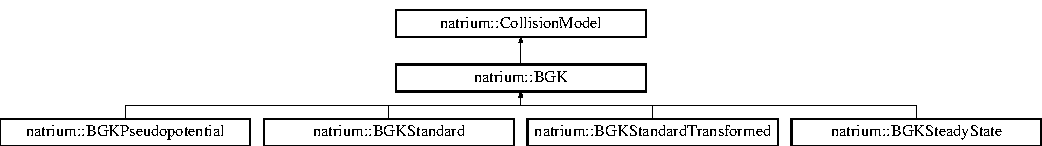
\includegraphics[height=1.96262cm]{classnatrium_1_1CollisionModel}
\end{center}
\end{figure}
\subsection*{Public Member Functions}
\begin{DoxyCompactItemize}
\item 
\hypertarget{classnatrium_1_1CollisionModel_a5e5254caec7f69000646886be11a34f8}{
{\bfseries CollisionModel} (const shared\_\-ptr$<$ \hyperlink{classnatrium_1_1Stencil}{Stencil} $>$ stencil)}
\label{classnatrium_1_1CollisionModel_a5e5254caec7f69000646886be11a34f8}

\item 
\hypertarget{classnatrium_1_1CollisionModel_ac6c6d95633d62209a04528af86807025}{
virtual void {\bfseries collideAll} (\hyperlink{classnatrium_1_1DistributionFunctions}{DistributionFunctions} \&f, distributed\_\-vector \&densities, vector$<$ distributed\_\-vector $>$ \&velocities, const dealii::IndexSet \&locally\_\-owned\_\-dofs, bool inInitializationProcedure=false) const =0}
\label{classnatrium_1_1CollisionModel_ac6c6d95633d62209a04528af86807025}

\item 
\hypertarget{classnatrium_1_1CollisionModel_aa0df0674bc26821d037323ac184fb52b}{
virtual void {\bfseries setTimeStep} (double dt)=0}
\label{classnatrium_1_1CollisionModel_aa0df0674bc26821d037323ac184fb52b}

\item 
\hypertarget{classnatrium_1_1CollisionModel_a482808bab1832ee06892630b8ead7dde}{
const shared\_\-ptr$<$ \hyperlink{classnatrium_1_1Stencil}{Stencil} $>$ \& {\bfseries getStencil} () const }
\label{classnatrium_1_1CollisionModel_a482808bab1832ee06892630b8ead7dde}

\item 
virtual double \hyperlink{classnatrium_1_1CollisionModel_ae1c879c87ac210a227a8e3da2d0ac385}{calculateDensity} (const vector$<$ double $>$ \&distributions) const 
\begin{DoxyCompactList}\small\item\em calculate macroscopic density \item\end{DoxyCompactList}\item 
virtual numeric\_\-vector \hyperlink{classnatrium_1_1CollisionModel_a90428f4c29916641de3de872803dde0f}{calculateVelocity} (const vector$<$ double $>$ \&distributions) const 
\begin{DoxyCompactList}\small\item\em calculate macroscopic velocity \item\end{DoxyCompactList}\item 
virtual void \hyperlink{classnatrium_1_1CollisionModel_a667f0e36da1bfb1c5102adb8f3afdcde}{calculateVelocity} (const vector$<$ double $>$ \&distributions, const double rho, numeric\_\-vector \&u) const 
\begin{DoxyCompactList}\small\item\em calculate macroscopic velocity; saves the double calculation of the density \item\end{DoxyCompactList}\item 
virtual double \hyperlink{classnatrium_1_1CollisionModel_a88b382d63da80e950bc58e8afad769a6}{getEquilibriumDistribution} (size\_\-t i, const numeric\_\-vector \&u, const double rho=1) const =0
\begin{DoxyCompactList}\small\item\em virtual function for the calculation of the equilibrium distribution \item\end{DoxyCompactList}\item 
virtual void \hyperlink{classnatrium_1_1CollisionModel_a296474961c4501bc23228be1d30ebf82}{getEquilibriumDistributions} (vector$<$ double $>$ \&feq, const numeric\_\-vector \&u, const double rho=1) const 
\begin{DoxyCompactList}\small\item\em function for the calculation of all equilibrium distributions \item\end{DoxyCompactList}\end{DoxyCompactItemize}


\subsection{Detailed Description}
Abstract collision model. Required to have a common parent of all template specializations of Collision. 

\subsection{Member Function Documentation}
\hypertarget{classnatrium_1_1CollisionModel_ae1c879c87ac210a227a8e3da2d0ac385}{
\index{natrium::CollisionModel@{natrium::CollisionModel}!calculateDensity@{calculateDensity}}
\index{calculateDensity@{calculateDensity}!natrium::CollisionModel@{natrium::CollisionModel}}
\subsubsection[{calculateDensity}]{\setlength{\rightskip}{0pt plus 5cm}virtual double natrium::CollisionModel::calculateDensity (const vector$<$ double $>$ \& {\em distributions}) const\hspace{0.3cm}{\ttfamily  \mbox{[}inline, virtual\mbox{]}}}}
\label{classnatrium_1_1CollisionModel_ae1c879c87ac210a227a8e3da2d0ac385}


calculate macroscopic density 
\begin{DoxyParams}{Parameters}
\item[\mbox{$\leftarrow$} {\em distributions}]particle distribution functions at a given point \end{DoxyParams}
\begin{DoxyReturn}{Returns}
macroscopic density (sum of all distributions) 
\end{DoxyReturn}


Reimplemented in \hyperlink{classnatrium_1_1BGKStandardTransformed_a58c4dc0c67ff4898c6555b614afc1ace}{natrium::BGKStandardTransformed}.\hypertarget{classnatrium_1_1CollisionModel_a667f0e36da1bfb1c5102adb8f3afdcde}{
\index{natrium::CollisionModel@{natrium::CollisionModel}!calculateVelocity@{calculateVelocity}}
\index{calculateVelocity@{calculateVelocity}!natrium::CollisionModel@{natrium::CollisionModel}}
\subsubsection[{calculateVelocity}]{\setlength{\rightskip}{0pt plus 5cm}virtual void natrium::CollisionModel::calculateVelocity (const vector$<$ double $>$ \& {\em distributions}, \/  const double {\em rho}, \/  numeric\_\-vector \& {\em u}) const\hspace{0.3cm}{\ttfamily  \mbox{[}inline, virtual\mbox{]}}}}
\label{classnatrium_1_1CollisionModel_a667f0e36da1bfb1c5102adb8f3afdcde}


calculate macroscopic velocity; saves the double calculation of the density \begin{DoxyNote}{Note}
more efficient 
\end{DoxyNote}

\begin{DoxyParams}{Parameters}
\item[\mbox{$\leftarrow$} {\em distributions}]particle distribution functions at a given point \item[\mbox{$\leftarrow$} {\em rho}]macroscopic density \item[\mbox{$\rightarrow$} {\em u}]macroscopic velocity \end{DoxyParams}
\hypertarget{classnatrium_1_1CollisionModel_a90428f4c29916641de3de872803dde0f}{
\index{natrium::CollisionModel@{natrium::CollisionModel}!calculateVelocity@{calculateVelocity}}
\index{calculateVelocity@{calculateVelocity}!natrium::CollisionModel@{natrium::CollisionModel}}
\subsubsection[{calculateVelocity}]{\setlength{\rightskip}{0pt plus 5cm}virtual numeric\_\-vector natrium::CollisionModel::calculateVelocity (const vector$<$ double $>$ \& {\em distributions}) const\hspace{0.3cm}{\ttfamily  \mbox{[}inline, virtual\mbox{]}}}}
\label{classnatrium_1_1CollisionModel_a90428f4c29916641de3de872803dde0f}


calculate macroscopic velocity 
\begin{DoxyParams}{Parameters}
\item[\mbox{$\leftarrow$} {\em distributions}]particle distribution functions at a given point \end{DoxyParams}
\begin{DoxyReturn}{Returns}
macroscopic velocity 
\end{DoxyReturn}
\hypertarget{classnatrium_1_1CollisionModel_a88b382d63da80e950bc58e8afad769a6}{
\index{natrium::CollisionModel@{natrium::CollisionModel}!getEquilibriumDistribution@{getEquilibriumDistribution}}
\index{getEquilibriumDistribution@{getEquilibriumDistribution}!natrium::CollisionModel@{natrium::CollisionModel}}
\subsubsection[{getEquilibriumDistribution}]{\setlength{\rightskip}{0pt plus 5cm}virtual double natrium::CollisionModel::getEquilibriumDistribution (size\_\-t {\em i}, \/  const numeric\_\-vector \& {\em u}, \/  const double {\em rho} = {\ttfamily 1}) const\hspace{0.3cm}{\ttfamily  \mbox{[}pure virtual\mbox{]}}}}
\label{classnatrium_1_1CollisionModel_a88b382d63da80e950bc58e8afad769a6}


virtual function for the calculation of the equilibrium distribution 
\begin{DoxyParams}{Parameters}
\item[{\em i}]index of the direction \item[{\em u}]macroscopic velocity \item[{\em rho}]macroscopic density \end{DoxyParams}
\begin{DoxyReturn}{Returns}
value of the equilibrium distribution 
\end{DoxyReturn}
\begin{DoxyNote}{Note}
The calculation can surely be done more efficiently by passing different arguments, e.g. u$\ast$u or u/(c$^\wedge$2) 
\end{DoxyNote}


Implemented in \hyperlink{classnatrium_1_1BGKPseudopotential_a63ce98e44a07466963fb123cac9dd905}{natrium::BGKPseudopotential}, \hyperlink{classnatrium_1_1BGKStandard_a3d45ef2fe5536bf14914f99297477754}{natrium::BGKStandard}, \hyperlink{classnatrium_1_1BGKStandardTransformed_a870465cc026f92c8ffba899af6f95634}{natrium::BGKStandardTransformed}, and \hyperlink{classnatrium_1_1BGKSteadyState_ad99d9159cc14b5897bea7f145c3b39ca}{natrium::BGKSteadyState}.\hypertarget{classnatrium_1_1CollisionModel_a296474961c4501bc23228be1d30ebf82}{
\index{natrium::CollisionModel@{natrium::CollisionModel}!getEquilibriumDistributions@{getEquilibriumDistributions}}
\index{getEquilibriumDistributions@{getEquilibriumDistributions}!natrium::CollisionModel@{natrium::CollisionModel}}
\subsubsection[{getEquilibriumDistributions}]{\setlength{\rightskip}{0pt plus 5cm}void natrium::CollisionModel::getEquilibriumDistributions (vector$<$ double $>$ \& {\em feq}, \/  const numeric\_\-vector \& {\em u}, \/  const double {\em rho} = {\ttfamily 1}) const\hspace{0.3cm}{\ttfamily  \mbox{[}virtual\mbox{]}}}}
\label{classnatrium_1_1CollisionModel_a296474961c4501bc23228be1d30ebf82}


function for the calculation of all equilibrium distributions 
\begin{DoxyParams}{Parameters}
\item[\mbox{$\rightarrow$} {\em feq}]vector of all equality distributions, must have size Q \item[\mbox{$\leftarrow$} {\em u}]macroscopic velocity \item[\mbox{$\leftarrow$} {\em rho}]macroscopic density \end{DoxyParams}
\begin{DoxyNote}{Note}
The calculation can surely be done more efficiently by passing different arguments, e.g. u$\ast$u or u/(c$^\wedge$2) 
\end{DoxyNote}


The documentation for this class was generated from the following files:\begin{DoxyCompactItemize}
\item 
/mnt/fdrive/akraem3m/workspace/NATriuM/src/library/natrium/collision/\hyperlink{CollisionModel_8h}{CollisionModel.h}\item 
/mnt/fdrive/akraem3m/workspace/NATriuM/src/library/natrium/collision/\hyperlink{CollisionModel_8cpp}{CollisionModel.cpp}\end{DoxyCompactItemize}

\hypertarget{classnatrium_1_1CouetteFlow2D}{\section{natrium\-:\-:Couette\-Flow2\-D Class Reference}
\label{classnatrium_1_1CouetteFlow2D}\index{natrium\-::\-Couette\-Flow2\-D@{natrium\-::\-Couette\-Flow2\-D}}
}


Description of a simple Couette Flow (regular channel flow in square domain). The domain is \mbox{[}0,1\mbox{]}$^\wedge$2. The top plate is moved with constant velocity. The domain consists of 8 x 8 = 64 Elements (contrast to Min and Lee, who have 6 x 6).  




{\ttfamily \#include $<$Couette\-Flow2\-D.\-h$>$}

Inheritance diagram for natrium\-:\-:Couette\-Flow2\-D\-:\begin{figure}[H]
\begin{center}
\leavevmode
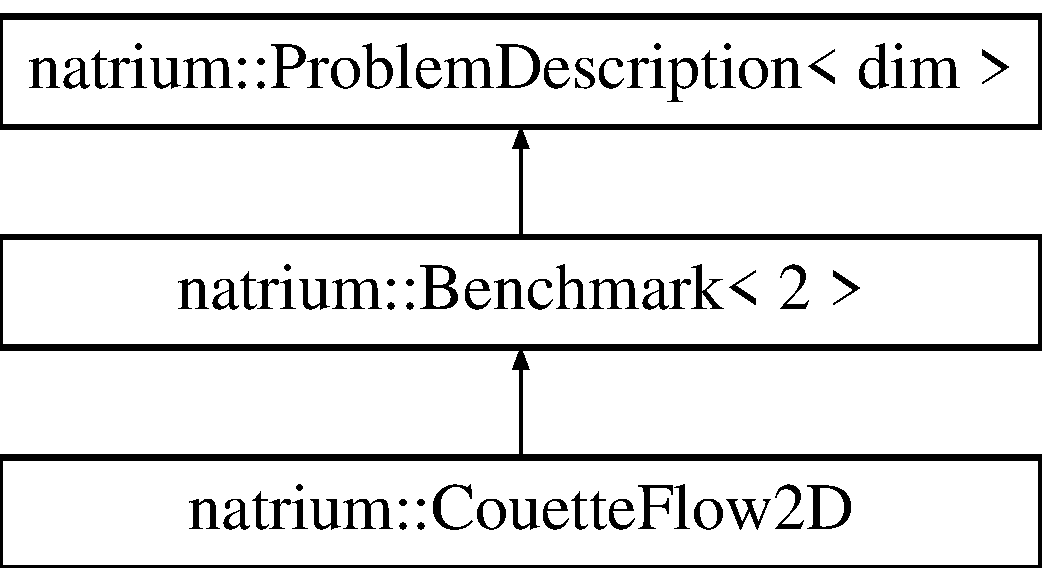
\includegraphics[height=3.000000cm]{classnatrium_1_1CouetteFlow2D}
\end{center}
\end{figure}
\subsection*{Public Member Functions}
\begin{DoxyCompactItemize}
\item 
\hyperlink{classnatrium_1_1CouetteFlow2D_a94e51b7eaff3998383f1d7dc07b994cb}{Couette\-Flow2\-D} (double viscosity, double top\-Plate\-Velocity, size\-\_\-t refinement\-Level, double L=1.\-0, double start\-Time=0.\-0, bool is\-Unstructured=false)
\begin{DoxyCompactList}\small\item\em constructor \end{DoxyCompactList}\item 
\hypertarget{classnatrium_1_1CouetteFlow2D_a97b61b0f71dc653427ba3db46e185873}{virtual \hyperlink{classnatrium_1_1CouetteFlow2D_a97b61b0f71dc653427ba3db46e185873}{$\sim$\-Couette\-Flow2\-D} ()}\label{classnatrium_1_1CouetteFlow2D_a97b61b0f71dc653427ba3db46e185873}

\begin{DoxyCompactList}\small\item\em destructor \end{DoxyCompactList}\item 
\hypertarget{classnatrium_1_1CouetteFlow2D_a3953d81acbab33424dfc4135930253df}{virtual void \hyperlink{classnatrium_1_1CouetteFlow2D_a3953d81acbab33424dfc4135930253df}{get\-Analytic\-Velocity} (const dealii\-::\-Point$<$ 2 $>$ \&x, double t, dealii\-::\-Point$<$ 2 $>$ \&velocity) const }\label{classnatrium_1_1CouetteFlow2D_a3953d81acbab33424dfc4135930253df}

\begin{DoxyCompactList}\small\item\em analytic solution of the Taylor-\/\-Green vortex \end{DoxyCompactList}\item 
\hypertarget{classnatrium_1_1CouetteFlow2D_a74429d98c455a0c06430a665505d8375}{virtual double {\bfseries get\-Characteristic\-Velocity} () const }\label{classnatrium_1_1CouetteFlow2D_a74429d98c455a0c06430a665505d8375}

\end{DoxyCompactItemize}


\subsection{Detailed Description}
Description of a simple Couette Flow (regular channel flow in square domain). The domain is \mbox{[}0,1\mbox{]}$^\wedge$2. The top plate is moved with constant velocity. The domain consists of 8 x 8 = 64 Elements (contrast to Min and Lee, who have 6 x 6). 

\begin{DoxyNote}{Note}
The analytic solution is obtained by a formula stated in Min and Lee (2011). 
\end{DoxyNote}


\subsection{Constructor \& Destructor Documentation}
\hypertarget{classnatrium_1_1CouetteFlow2D_a94e51b7eaff3998383f1d7dc07b994cb}{\index{natrium\-::\-Couette\-Flow2\-D@{natrium\-::\-Couette\-Flow2\-D}!Couette\-Flow2\-D@{Couette\-Flow2\-D}}
\index{Couette\-Flow2\-D@{Couette\-Flow2\-D}!natrium::CouetteFlow2D@{natrium\-::\-Couette\-Flow2\-D}}
\subsubsection[{Couette\-Flow2\-D}]{\setlength{\rightskip}{0pt plus 5cm}natrium\-::\-Couette\-Flow2\-D\-::\-Couette\-Flow2\-D (
\begin{DoxyParamCaption}
\item[{double}]{viscosity, }
\item[{double}]{top\-Plate\-Velocity, }
\item[{size\-\_\-t}]{refinement\-Level, }
\item[{double}]{L = {\ttfamily 1.0}, }
\item[{double}]{start\-Time = {\ttfamily 0.0}, }
\item[{bool}]{is\-Unstructured = {\ttfamily false}}
\end{DoxyParamCaption}
)}}\label{classnatrium_1_1CouetteFlow2D_a94e51b7eaff3998383f1d7dc07b994cb}


constructor 

apply boundary values 

The documentation for this class was generated from the following files\-:\begin{DoxyCompactItemize}
\item 
/home/kraemer/eclipse\-\_\-workspace/\-N\-A\-Triu\-M/src/examples/step-\/2/\hyperlink{CouetteFlow2D_8h}{Couette\-Flow2\-D.\-h}\item 
/home/kraemer/eclipse\-\_\-workspace/\-N\-A\-Triu\-M/src/examples/step-\/2/\hyperlink{CouetteFlow2D_8cpp}{Couette\-Flow2\-D.\-cpp}\end{DoxyCompactItemize}

\hypertarget{classnatrium_1_1D2Q9IncompressibleModel}{\section{natrium\-:\-:D2\-Q9\-Incompressible\-Model Class Reference}
\label{classnatrium_1_1D2Q9IncompressibleModel}\index{natrium\-::\-D2\-Q9\-Incompressible\-Model@{natrium\-::\-D2\-Q9\-Incompressible\-Model}}
}


D2\-Q9 model description for incompressible flow.  




{\ttfamily \#include $<$D2\-Q9\-Incompressible\-Model.\-h$>$}

Inheritance diagram for natrium\-:\-:D2\-Q9\-Incompressible\-Model\-:\begin{figure}[H]
\begin{center}
\leavevmode
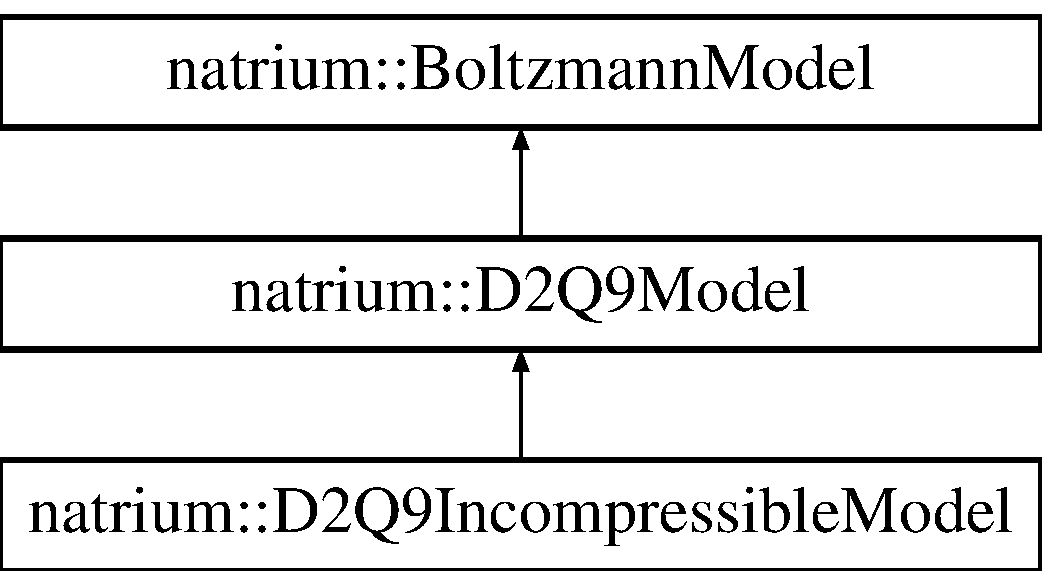
\includegraphics[height=3.000000cm]{classnatrium_1_1D2Q9IncompressibleModel}
\end{center}
\end{figure}
\subsection*{Public Member Functions}
\begin{DoxyCompactItemize}
\item 
\hypertarget{classnatrium_1_1D2Q9IncompressibleModel_a2ebdd3442edd4e3f38798a99b8413fcb}{\hyperlink{classnatrium_1_1D2Q9IncompressibleModel_a2ebdd3442edd4e3f38798a99b8413fcb}{D2\-Q9\-Incompressible\-Model} (double scaling=1)}\label{classnatrium_1_1D2Q9IncompressibleModel_a2ebdd3442edd4e3f38798a99b8413fcb}

\begin{DoxyCompactList}\small\item\em constructor \end{DoxyCompactList}\item 
virtual \hyperlink{classnatrium_1_1D2Q9IncompressibleModel_a6e757941f7ca2c5a6148893147211724}{$\sim$\-D2\-Q9\-Incompressible\-Model} ()
\begin{DoxyCompactList}\small\item\em destructor \end{DoxyCompactList}\item 
virtual double \hyperlink{classnatrium_1_1D2Q9IncompressibleModel_ac461ec3ce0f4ecd742dfbdfb1bce7d5a}{get\-Equilibrium\-Distribution} (size\-\_\-t i, const numeric\-\_\-vector \&u, const double rho=1) const 
\begin{DoxyCompactList}\small\item\em function for the calculation of the equilibrium distribution in the incompressible D2\-Q9 model \end{DoxyCompactList}\end{DoxyCompactItemize}
\subsection*{Additional Inherited Members}


\subsection{Detailed Description}
D2\-Q9 model description for incompressible flow. 

\subsection{Constructor \& Destructor Documentation}
\hypertarget{classnatrium_1_1D2Q9IncompressibleModel_a6e757941f7ca2c5a6148893147211724}{\index{natrium\-::\-D2\-Q9\-Incompressible\-Model@{natrium\-::\-D2\-Q9\-Incompressible\-Model}!$\sim$\-D2\-Q9\-Incompressible\-Model@{$\sim$\-D2\-Q9\-Incompressible\-Model}}
\index{$\sim$\-D2\-Q9\-Incompressible\-Model@{$\sim$\-D2\-Q9\-Incompressible\-Model}!natrium::D2Q9IncompressibleModel@{natrium\-::\-D2\-Q9\-Incompressible\-Model}}
\subsubsection[{$\sim$\-D2\-Q9\-Incompressible\-Model}]{\setlength{\rightskip}{0pt plus 5cm}natrium\-::\-D2\-Q9\-Incompressible\-Model\-::$\sim$\-D2\-Q9\-Incompressible\-Model (
\begin{DoxyParamCaption}
{}
\end{DoxyParamCaption}
)\hspace{0.3cm}{\ttfamily [virtual]}}}\label{classnatrium_1_1D2Q9IncompressibleModel_a6e757941f7ca2c5a6148893147211724}


destructor 

constructor

destructor 

\subsection{Member Function Documentation}
\hypertarget{classnatrium_1_1D2Q9IncompressibleModel_ac461ec3ce0f4ecd742dfbdfb1bce7d5a}{\index{natrium\-::\-D2\-Q9\-Incompressible\-Model@{natrium\-::\-D2\-Q9\-Incompressible\-Model}!get\-Equilibrium\-Distribution@{get\-Equilibrium\-Distribution}}
\index{get\-Equilibrium\-Distribution@{get\-Equilibrium\-Distribution}!natrium::D2Q9IncompressibleModel@{natrium\-::\-D2\-Q9\-Incompressible\-Model}}
\subsubsection[{get\-Equilibrium\-Distribution}]{\setlength{\rightskip}{0pt plus 5cm}virtual double natrium\-::\-D2\-Q9\-Incompressible\-Model\-::get\-Equilibrium\-Distribution (
\begin{DoxyParamCaption}
\item[{size\-\_\-t}]{i, }
\item[{const numeric\-\_\-vector \&}]{u, }
\item[{const double}]{rho = {\ttfamily 1}}
\end{DoxyParamCaption}
) const\hspace{0.3cm}{\ttfamily [inline]}, {\ttfamily [virtual]}}}\label{classnatrium_1_1D2Q9IncompressibleModel_ac461ec3ce0f4ecd742dfbdfb1bce7d5a}


function for the calculation of the equilibrium distribution in the incompressible D2\-Q9 model 


\begin{DoxyParams}{Parameters}
{\em i} & index of the direction \\
\hline
{\em u} & macroscopic velocity \\
\hline
{\em rho} & macroscopic density \\
\hline
\end{DoxyParams}
\begin{DoxyReturn}{Returns}
value of the equilibrium distribution 
\end{DoxyReturn}
\begin{DoxyNote}{Note}
The calculation can surely be done more efficiently by passing different arguments, e.\-g. u$\ast$u or u/(c$^\wedge$2) 
\end{DoxyNote}


Implements \hyperlink{classnatrium_1_1BoltzmannModel_ad482e26c4df3014e4b1447ee6cbb44ff}{natrium\-::\-Boltzmann\-Model}.



The documentation for this class was generated from the following files\-:\begin{DoxyCompactItemize}
\item 
/home/kraemer/eclipse\-\_\-workspace/\-N\-A\-Triu\-M/src/natrium/boltzmannmodels/D2\-Q9\-Incompressible\-Model.\-h\item 
/home/kraemer/eclipse\-\_\-workspace/\-N\-A\-Triu\-M/src/natrium/boltzmannmodels/D2\-Q9\-Incompressible\-Model.\-cpp\end{DoxyCompactItemize}

\hypertarget{classnatrium_1_1D2Q9Model}{\section{natrium\-:\-:D2\-Q9\-Model Class Reference}
\label{classnatrium_1_1D2Q9Model}\index{natrium\-::\-D2\-Q9\-Model@{natrium\-::\-D2\-Q9\-Model}}
}


D2\-Q9 Model.  




{\ttfamily \#include $<$D2\-Q9\-Model.\-h$>$}

Inheritance diagram for natrium\-:\-:D2\-Q9\-Model\-:\begin{figure}[H]
\begin{center}
\leavevmode
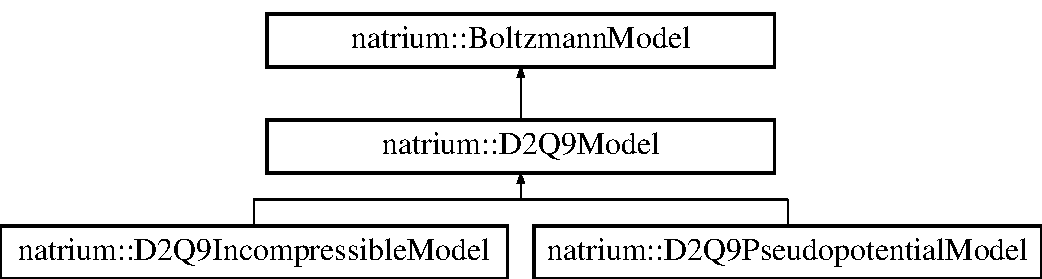
\includegraphics[height=3.000000cm]{classnatrium_1_1D2Q9Model}
\end{center}
\end{figure}
\subsection*{Public Member Functions}
\begin{DoxyCompactItemize}
\item 
\hypertarget{classnatrium_1_1D2Q9Model_af498c14d311e9172d96b5d962ccc5202}{\hyperlink{classnatrium_1_1D2Q9Model_af498c14d311e9172d96b5d962ccc5202}{D2\-Q9\-Model} (double scaling)}\label{classnatrium_1_1D2Q9Model_af498c14d311e9172d96b5d962ccc5202}

\begin{DoxyCompactList}\small\item\em constructor \end{DoxyCompactList}\item 
\hypertarget{classnatrium_1_1D2Q9Model_aec7d8c160f430e14fbede9ecda368797}{virtual \hyperlink{classnatrium_1_1D2Q9Model_aec7d8c160f430e14fbede9ecda368797}{$\sim$\-D2\-Q9\-Model} ()}\label{classnatrium_1_1D2Q9Model_aec7d8c160f430e14fbede9ecda368797}

\begin{DoxyCompactList}\small\item\em destructor \end{DoxyCompactList}\item 
\hypertarget{classnatrium_1_1D2Q9Model_ac9b53eb73e84ecd13afcf9f3a0b0e195}{virtual double {\bfseries get\-Speed\-Of\-Sound} () const }\label{classnatrium_1_1D2Q9Model_ac9b53eb73e84ecd13afcf9f3a0b0e195}

\item 
\hypertarget{classnatrium_1_1D2Q9Model_aa83e54b682ec7081c298324ee9688a8e}{virtual double {\bfseries get\-Speed\-Of\-Sound\-Square} () const }\label{classnatrium_1_1D2Q9Model_aa83e54b682ec7081c298324ee9688a8e}

\item 
\hypertarget{classnatrium_1_1D2Q9Model_ae29e3df458e24802467ca9c2209cc0ca}{virtual size\-\_\-t {\bfseries get\-Index\-Of\-Opposite\-Direction} (size\-\_\-t index) const }\label{classnatrium_1_1D2Q9Model_ae29e3df458e24802467ca9c2209cc0ca}

\end{DoxyCompactItemize}
\subsection*{Static Public Attributes}
\begin{DoxyCompactItemize}
\item 
\hypertarget{classnatrium_1_1D2Q9Model_a81532a1067ba5f280698a1a84711ede5}{static const size\-\_\-t \hyperlink{classnatrium_1_1D2Q9Model_a81532a1067ba5f280698a1a84711ede5}{D} = 2}\label{classnatrium_1_1D2Q9Model_a81532a1067ba5f280698a1a84711ede5}

\begin{DoxyCompactList}\small\item\em D. \end{DoxyCompactList}\item 
\hypertarget{classnatrium_1_1D2Q9Model_ad3d102dfb9c8ad7b56a8f82c3f4286f6}{static const size\-\_\-t \hyperlink{classnatrium_1_1D2Q9Model_ad3d102dfb9c8ad7b56a8f82c3f4286f6}{Q} = 9}\label{classnatrium_1_1D2Q9Model_ad3d102dfb9c8ad7b56a8f82c3f4286f6}

\begin{DoxyCompactList}\small\item\em Q. \end{DoxyCompactList}\end{DoxyCompactItemize}
\subsection*{Protected Attributes}
\begin{DoxyCompactItemize}
\item 
\hypertarget{classnatrium_1_1D2Q9Model_ab212c0c04921591f16c1970d93878cf9}{const double \hyperlink{classnatrium_1_1D2Q9Model_ab212c0c04921591f16c1970d93878cf9}{m\-\_\-speed\-Of\-Sound}}\label{classnatrium_1_1D2Q9Model_ab212c0c04921591f16c1970d93878cf9}

\begin{DoxyCompactList}\small\item\em speed of sound \end{DoxyCompactList}\item 
\hypertarget{classnatrium_1_1D2Q9Model_afa28316438de5055d51674d89a0075ba}{const double \hyperlink{classnatrium_1_1D2Q9Model_afa28316438de5055d51674d89a0075ba}{m\-\_\-speed\-Of\-Sound\-Square}}\label{classnatrium_1_1D2Q9Model_afa28316438de5055d51674d89a0075ba}

\begin{DoxyCompactList}\small\item\em (speed of sound)$^\wedge$2 \end{DoxyCompactList}\end{DoxyCompactItemize}


\subsection{Detailed Description}
D2\-Q9 Model. 

The documentation for this class was generated from the following files\-:\begin{DoxyCompactItemize}
\item 
/home/kraemer/eclipse\-\_\-workspace/\-N\-A\-Triu\-M/src/natrium/boltzmannmodels/\hyperlink{D2Q9Model_8h}{D2\-Q9\-Model.\-h}\item 
/home/kraemer/eclipse\-\_\-workspace/\-N\-A\-Triu\-M/src/natrium/boltzmannmodels/\hyperlink{D2Q9Model_8cpp}{D2\-Q9\-Model.\-cpp}\end{DoxyCompactItemize}

\hypertarget{classnatrium_1_1DataMinLee2011}{\section{natrium\-:\-:\-Data\-Min\-Lee2011$<$ dim $>$ \-Class \-Template \-Reference}
\label{classnatrium_1_1DataMinLee2011}\index{natrium\-::\-Data\-Min\-Lee2011$<$ dim $>$@{natrium\-::\-Data\-Min\-Lee2011$<$ dim $>$}}
}


\-Global data which is used, e.\-g., by \-Min and \-Lee (2011)\-: \-A spectral-\/element discontinuous \-Galerkin lattice \-Boltzmann method for nearly incompressible flows, \-J\-C\-P 230 pp. 245-\/259. including particle distributions f, system matrix \-L, diagonal mass matrix \-M, gradient matrices \-Dx, \-Dy, (\-Dz) and boundary matrix \-R.  




{\ttfamily \#include $<$\-Data\-Min\-Lee2011.\-h$>$}

\-Inheritance diagram for natrium\-:\-:\-Data\-Min\-Lee2011$<$ dim $>$\-:\begin{figure}[H]
\begin{center}
\leavevmode
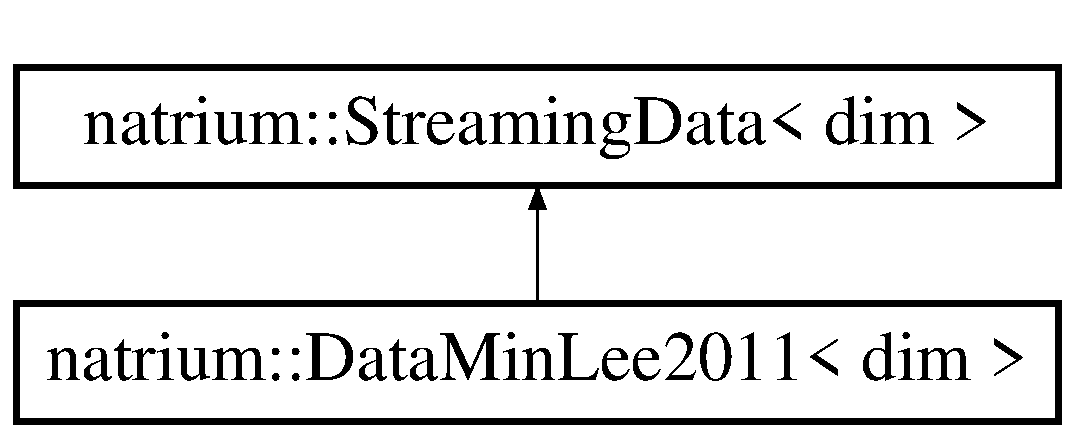
\includegraphics[height=2.000000cm]{classnatrium_1_1DataMinLee2011}
\end{center}
\end{figure}
\subsection*{\-Public \-Member \-Functions}
\begin{DoxyCompactItemize}
\item 
\hypertarget{classnatrium_1_1DataMinLee2011_aaaae9305f9878aa2f2e19dfd2293ebdc}{\hyperlink{classnatrium_1_1DataMinLee2011_aaaae9305f9878aa2f2e19dfd2293ebdc}{\-Data\-Min\-Lee2011} ()}\label{classnatrium_1_1DataMinLee2011_aaaae9305f9878aa2f2e19dfd2293ebdc}

\begin{DoxyCompactList}\small\item\em constructor \end{DoxyCompactList}\item 
\hypertarget{classnatrium_1_1DataMinLee2011_a248508156e259f7278e7770d9e3c4c98}{virtual \hyperlink{classnatrium_1_1DataMinLee2011_a248508156e259f7278e7770d9e3c4c98}{$\sim$\-Data\-Min\-Lee2011} ()}\label{classnatrium_1_1DataMinLee2011_a248508156e259f7278e7770d9e3c4c98}

\begin{DoxyCompactList}\small\item\em destructor \end{DoxyCompactList}\end{DoxyCompactItemize}


\subsection{\-Detailed \-Description}
\subsubsection*{template$<$int dim$>$class natrium\-::\-Data\-Min\-Lee2011$<$ dim $>$}

\-Global data which is used, e.\-g., by \-Min and \-Lee (2011)\-: \-A spectral-\/element discontinuous \-Galerkin lattice \-Boltzmann method for nearly incompressible flows, \-J\-C\-P 230 pp. 245-\/259. including particle distributions f, system matrix \-L, diagonal mass matrix \-M, gradient matrices \-Dx, \-Dy, (\-Dz) and boundary matrix \-R. 


\begin{DoxyTemplParams}{\-Template Parameters}
{\em dim} & \-The dimension of the flow (2 or 3). \\
\hline
\end{DoxyTemplParams}


\-The documentation for this class was generated from the following file\-:\begin{DoxyCompactItemize}
\item 
/home/kraemer/eclipse\-\_\-workspace/\-N\-A\-Triu\-M/src/streamingdata/\hyperlink{DataMinLee2011_8h}{\-Data\-Min\-Lee2011.\-h}\end{DoxyCompactItemize}

\hypertarget{classnatrium_1_1ExponentialTimeIntegrator}{
\section{natrium::ExponentialTimeIntegrator$<$ MATRIX, VECTOR $>$ Class Template Reference}
\label{classnatrium_1_1ExponentialTimeIntegrator}\index{natrium::ExponentialTimeIntegrator@{natrium::ExponentialTimeIntegrator}}
}


Exponential time integration scheme for the solution of f' = L$\ast$f, as used in Uga etal. (2012) Spectral-\/element discontinuous Galerkin lattice Boltzmann simulation of flow past two cylinders in tandem with an exponential time integrator, CMWA 65 pp. 239-\/251.  


{\ttfamily \#include $<$ExponentialTimeIntegrator.h$>$}Inheritance diagram for natrium::ExponentialTimeIntegrator$<$ MATRIX, VECTOR $>$::\begin{figure}[H]
\begin{center}
\leavevmode
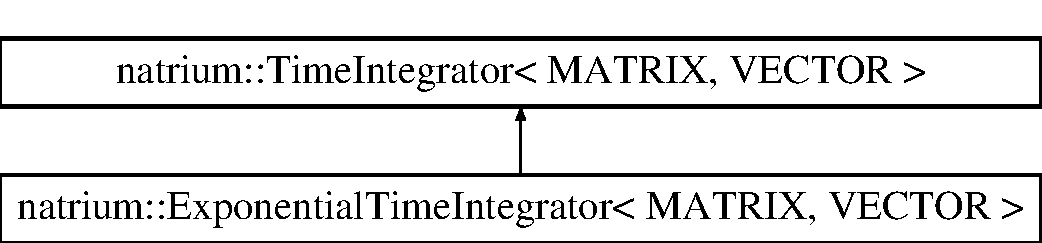
\includegraphics[height=2cm]{classnatrium_1_1ExponentialTimeIntegrator}
\end{center}
\end{figure}
\subsection*{Public Member Functions}
\begin{DoxyCompactItemize}
\item 
\hypertarget{classnatrium_1_1ExponentialTimeIntegrator_a3a3e7b0c53b5c083dbdb7b3d625d8087}{
\hyperlink{classnatrium_1_1ExponentialTimeIntegrator_a3a3e7b0c53b5c083dbdb7b3d625d8087}{ExponentialTimeIntegrator} (double timeStepSize)}
\label{classnatrium_1_1ExponentialTimeIntegrator_a3a3e7b0c53b5c083dbdb7b3d625d8087}

\begin{DoxyCompactList}\small\item\em constructor \item\end{DoxyCompactList}\item 
\hypertarget{classnatrium_1_1ExponentialTimeIntegrator_a7da2892aead7c5e1fec82be549dcb37b}{
{\bfseries ExponentialTimeIntegrator} (double timeStepSize, size\_\-t numberOfBlocks)}
\label{classnatrium_1_1ExponentialTimeIntegrator_a7da2892aead7c5e1fec82be549dcb37b}

\item 
\hypertarget{classnatrium_1_1ExponentialTimeIntegrator_ad85e62117ec3dbfebfbccd6ad1135d8c}{
virtual \hyperlink{classnatrium_1_1ExponentialTimeIntegrator_ad85e62117ec3dbfebfbccd6ad1135d8c}{$\sim$ExponentialTimeIntegrator} ()}
\label{classnatrium_1_1ExponentialTimeIntegrator_ad85e62117ec3dbfebfbccd6ad1135d8c}

\begin{DoxyCompactList}\small\item\em destructor \item\end{DoxyCompactList}\item 
virtual double \hyperlink{classnatrium_1_1ExponentialTimeIntegrator_ae0a9cff9bdafab123016db72d1439ef8}{step} (VECTOR \&f, const MATRIX \&systemMatrix, const VECTOR \&systemVector, double t=0, double dt=0)
\begin{DoxyCompactList}\small\item\em make one time integration step on f: \[ \frac{df}{dt} = Af+b \]. \item\end{DoxyCompactList}\item 
\hypertarget{classnatrium_1_1ExponentialTimeIntegrator_a7b68727897acae02ff025c39a56a4bf6}{
{\footnotesize template$<$$>$ }\\{\bfseries ExponentialTimeIntegrator} (double timeStepSize)}
\label{classnatrium_1_1ExponentialTimeIntegrator_a7b68727897acae02ff025c39a56a4bf6}

\item 
\hypertarget{classnatrium_1_1ExponentialTimeIntegrator_acbd606f38f9c5c0b4cb9b9fc817f1186}{
{\footnotesize template$<$$>$ }\\{\bfseries ExponentialTimeIntegrator} (double timeStepSize, size\_\-t)}
\label{classnatrium_1_1ExponentialTimeIntegrator_acbd606f38f9c5c0b4cb9b9fc817f1186}

\item 
\hypertarget{classnatrium_1_1ExponentialTimeIntegrator_a9fbf0f44e2d68eab2df6d767e6f08c77}{
{\footnotesize template$<$$>$ }\\{\bfseries ExponentialTimeIntegrator} (double timeStepSize)}
\label{classnatrium_1_1ExponentialTimeIntegrator_a9fbf0f44e2d68eab2df6d767e6f08c77}

\item 
\hypertarget{classnatrium_1_1ExponentialTimeIntegrator_a716b2f09970240253c9175e3ad5e3965}{
{\footnotesize template$<$$>$ }\\{\bfseries ExponentialTimeIntegrator} (double timeStepSize, size\_\-t)}
\label{classnatrium_1_1ExponentialTimeIntegrator_a716b2f09970240253c9175e3ad5e3965}

\item 
\hypertarget{classnatrium_1_1ExponentialTimeIntegrator_a04d6a47d38318ab92ba4bd22b834d6c3}{
{\footnotesize template$<$$>$ }\\dealii::IndexSet {\bfseries getIndexSet} (const distributed\_\-sparse\_\-matrix \&m)}
\label{classnatrium_1_1ExponentialTimeIntegrator_a04d6a47d38318ab92ba4bd22b834d6c3}

\item 
\hypertarget{classnatrium_1_1ExponentialTimeIntegrator_aa58b4f252c2f19808f10102d60eed3a9}{
{\footnotesize template$<$$>$ }\\dealii::IndexSet {\bfseries getIndexSet} (const distributed\_\-sparse\_\-block\_\-matrix \&m)}
\label{classnatrium_1_1ExponentialTimeIntegrator_aa58b4f252c2f19808f10102d60eed3a9}

\item 
\hypertarget{classnatrium_1_1ExponentialTimeIntegrator_a6ea6d696834a57e0e8af03558ffc1d5b}{
{\footnotesize template$<$$>$ }\\dealii::IndexSet {\bfseries getIndexSet} (const sparse\_\-matrix \&m)}
\label{classnatrium_1_1ExponentialTimeIntegrator_a6ea6d696834a57e0e8af03558ffc1d5b}

\item 
\hypertarget{classnatrium_1_1ExponentialTimeIntegrator_a0d43b0a3b92ced2b9b7755549742baa0}{
{\footnotesize template$<$$>$ }\\dealii::IndexSet {\bfseries getIndexSet} (const sparse\_\-block\_\-matrix \&m)}
\label{classnatrium_1_1ExponentialTimeIntegrator_a0d43b0a3b92ced2b9b7755549742baa0}

\end{DoxyCompactItemize}


\subsection{Detailed Description}
\subsubsection*{template$<$class MATRIX, class VECTOR$>$ class natrium::ExponentialTimeIntegrator$<$ MATRIX, VECTOR $>$}

Exponential time integration scheme for the solution of f' = L$\ast$f, as used in Uga etal. (2012) Spectral-\/element discontinuous Galerkin lattice Boltzmann simulation of flow past two cylinders in tandem with an exponential time integrator, CMWA 65 pp. 239-\/251. 

\subsection{Member Function Documentation}
\hypertarget{classnatrium_1_1ExponentialTimeIntegrator_ae0a9cff9bdafab123016db72d1439ef8}{
\index{natrium::ExponentialTimeIntegrator@{natrium::ExponentialTimeIntegrator}!step@{step}}
\index{step@{step}!natrium::ExponentialTimeIntegrator@{natrium::ExponentialTimeIntegrator}}
\subsubsection[{step}]{\setlength{\rightskip}{0pt plus 5cm}template$<$class MATRIX , class VECTOR $>$ double {\bf natrium::ExponentialTimeIntegrator}$<$ MATRIX, VECTOR $>$::step (VECTOR \& {\em f}, \/  const MATRIX \& {\em systemMatrix}, \/  const VECTOR \& {\em systemVector}, \/  double {\em t} = {\ttfamily 0}, \/  double {\em dt} = {\ttfamily 0})\hspace{0.3cm}{\ttfamily  \mbox{[}inline, virtual\mbox{]}}}}
\label{classnatrium_1_1ExponentialTimeIntegrator_ae0a9cff9bdafab123016db72d1439ef8}


make one time integration step on f: \[ \frac{df}{dt} = Af+b \]. 
\begin{DoxyParams}{Parameters}
\item[{\em in/out\mbox{]}}]f Vector of degrees of freedom \item[\mbox{$\leftarrow$} {\em systemMatrix}]Matrix A \item[\mbox{$\leftarrow$} {\em systemVector}]Vector b \item[\mbox{$\leftarrow$} {\em double}]t global time \item[\mbox{$\leftarrow$} {\em double}]dt time step size. Required to interface deal.II's embedded RK methods \end{DoxyParams}
\begin{DoxyReturn}{Returns}
new global time 
\end{DoxyReturn}
\begin{DoxyNote}{Note}
fully virtual method. Overloaded by subclasses. 
\end{DoxyNote}


Implements \hyperlink{classnatrium_1_1TimeIntegrator_a1c438e41d183d172d524aa5dc97785fb}{natrium::TimeIntegrator$<$ MATRIX, VECTOR $>$}.

The documentation for this class was generated from the following files:\begin{DoxyCompactItemize}
\item 
/mnt/fdrive/akraem3m/workspace/NATriuM/src/library/natrium/timeintegration/ExponentialTimeIntegrator.h\item 
/mnt/fdrive/akraem3m/workspace/NATriuM/src/library/natrium/timeintegration/\hyperlink{ExponentialTimeIntegrator_8cpp}{ExponentialTimeIntegrator.cpp}\end{DoxyCompactItemize}

\hypertarget{classnatrium_1_1Math}{\section{natrium\-:\-:\-Math \-Class \-Reference}
\label{classnatrium_1_1Math}\index{natrium\-::\-Math@{natrium\-::\-Math}}
}


class which contains basic math functions  




{\ttfamily \#include $<$\-Basic\-Names.\-h$>$}

\subsection*{\-Static \-Public \-Member \-Functions}
\begin{DoxyCompactItemize}
\item 
\hypertarget{classnatrium_1_1Math_acb9f9cb7ff053ff86da3cf730a78fc3f}{static float\-\_\-t \hyperlink{classnatrium_1_1Math_acb9f9cb7ff053ff86da3cf730a78fc3f}{scalar\-\_\-product} (const numeric\-\_\-vector \&x, const numeric\-\_\-vector \&y)}\label{classnatrium_1_1Math_acb9f9cb7ff053ff86da3cf730a78fc3f}

\begin{DoxyCompactList}\small\item\em scalar product \end{DoxyCompactList}\item 
\hypertarget{classnatrium_1_1Math_a3396e401ecdf6eaea63441e4ab87e67d}{static void \hyperlink{classnatrium_1_1Math_a3396e401ecdf6eaea63441e4ab87e67d}{scale\-\_\-vector} (float\-\_\-t a, numeric\-\_\-vector \&x)}\label{classnatrium_1_1Math_a3396e401ecdf6eaea63441e4ab87e67d}

\begin{DoxyCompactList}\small\item\em scale existing vector \end{DoxyCompactList}\item 
\hypertarget{classnatrium_1_1Math_a866bc6361557248b9b6e2d8aac6696f5}{static numeric\-\_\-vector \hyperlink{classnatrium_1_1Math_a866bc6361557248b9b6e2d8aac6696f5}{scalar\-\_\-vector} (float\-\_\-t a, const numeric\-\_\-vector \&x)}\label{classnatrium_1_1Math_a866bc6361557248b9b6e2d8aac6696f5}

\begin{DoxyCompactList}\small\item\em scalar times vector \end{DoxyCompactList}\item 
\hypertarget{classnatrium_1_1Math_abf43ba6f35909ea95ceadc2c8eb33aa6}{static void {\bfseries add\-\_\-vector} (numeric\-\_\-vector \&x, const numeric\-\_\-vector \&y)}\label{classnatrium_1_1Math_abf43ba6f35909ea95ceadc2c8eb33aa6}

\item 
\hypertarget{classnatrium_1_1Math_a20f4b206876293f69412c5c37299c412}{static float\-\_\-t {\bfseries euclidean\-\_\-norm} (numeric\-\_\-vector \&x)}\label{classnatrium_1_1Math_a20f4b206876293f69412c5c37299c412}

\item 
\hypertarget{classnatrium_1_1Math_a70941f44aae05e58f726edafc2883889}{static float\-\_\-t {\bfseries by\-\_\-two} (float\-\_\-t a)}\label{classnatrium_1_1Math_a70941f44aae05e58f726edafc2883889}

\end{DoxyCompactItemize}


\subsection{\-Detailed \-Description}
class which contains basic math functions 

\-The documentation for this class was generated from the following file\-:\begin{DoxyCompactItemize}
\item 
/home/kraemer/eclipse\-\_\-workspace/\-N\-A\-Triu\-M/src/utilities/\hyperlink{BasicNames_8h}{\-Basic\-Names.\-h}\end{DoxyCompactItemize}

\hypertarget{classnatrium_1_1ProblemDescription}{\section{natrium\-:\-:Problem\-Description$<$ dim $>$ Class Template Reference}
\label{classnatrium_1_1ProblemDescription}\index{natrium\-::\-Problem\-Description$<$ dim $>$@{natrium\-::\-Problem\-Description$<$ dim $>$}}
}


Abstract class for the description of a C\-F\-D problem. The description includes the computational mesh, boundary description, viscosity and initial values.  




{\ttfamily \#include $<$Problem\-Description.\-h$>$}

\subsection*{Public Member Functions}
\begin{DoxyCompactItemize}
\item 
\hypertarget{classnatrium_1_1ProblemDescription_aae378c7eb216b616de56dfcd162c02c2}{\hyperlink{classnatrium_1_1ProblemDescription_aae378c7eb216b616de56dfcd162c02c2}{Problem\-Description} (shared\-\_\-ptr$<$ dealii\-::\-Triangulation$<$ dim $>$ $>$ triangulation, double viscosity, double characteristic\-Length)}\label{classnatrium_1_1ProblemDescription_aae378c7eb216b616de56dfcd162c02c2}

\begin{DoxyCompactList}\small\item\em constructor \end{DoxyCompactList}\item 
\hypertarget{classnatrium_1_1ProblemDescription_a5270994970ddbd9f6fc98f292c1ccc0e}{virtual \hyperlink{classnatrium_1_1ProblemDescription_a5270994970ddbd9f6fc98f292c1ccc0e}{$\sim$\-Problem\-Description} ()}\label{classnatrium_1_1ProblemDescription_a5270994970ddbd9f6fc98f292c1ccc0e}

\begin{DoxyCompactList}\small\item\em destructor \end{DoxyCompactList}\item 
\hypertarget{classnatrium_1_1ProblemDescription_a69d3b6c08733468e6c9c152ce4f83585}{const shared\-\_\-ptr\\*
$<$ dealii\-::\-Triangulation$<$ dim $>$ $>$ \& {\bfseries get\-Triangulation} () const }\label{classnatrium_1_1ProblemDescription_a69d3b6c08733468e6c9c152ce4f83585}

\item 
\hypertarget{classnatrium_1_1ProblemDescription_abb061fe78c8d289fe2a4a9000015d842}{const shared\-\_\-ptr\\*
$<$ \hyperlink{classnatrium_1_1BoundaryCollection}{Boundary\-Collection}$<$ dim $>$ $>$ \& {\bfseries get\-Boundaries} () const }\label{classnatrium_1_1ProblemDescription_abb061fe78c8d289fe2a4a9000015d842}

\item 
virtual void \hyperlink{classnatrium_1_1ProblemDescription_ab4ccefafd2888510038259445076fed6}{apply\-Initial\-Densities} (distributed\-\_\-vector \&initial\-Densities, vector$<$ dealii\-::\-Point$<$ dim $>$ $>$ \&support\-Points) const =0
\begin{DoxyCompactList}\small\item\em set initial densities \end{DoxyCompactList}\item 
virtual void \hyperlink{classnatrium_1_1ProblemDescription_a28306325c69e7d2086a3dd7f8c514b21}{apply\-Initial\-Velocities} (vector$<$ distributed\-\_\-vector $>$ \&initial\-Velocities, vector$<$ dealii\-::\-Point$<$ dim $>$ $>$ \&support\-Points) const =0
\begin{DoxyCompactList}\small\item\em set initial velocities \end{DoxyCompactList}\item 
\hypertarget{classnatrium_1_1ProblemDescription_ae588b1e0ce4dd89e2fcfbb0c191b1c41}{void {\bfseries set\-Triangulation} (const shared\-\_\-ptr$<$ dealii\-::\-Triangulation$<$ dim $>$ $>$ \&triangulation)}\label{classnatrium_1_1ProblemDescription_ae588b1e0ce4dd89e2fcfbb0c191b1c41}

\item 
\hypertarget{classnatrium_1_1ProblemDescription_aadca2aac3953fa44bf9ce9cf43dc0417}{void {\bfseries set\-Boundaries} (const shared\-\_\-ptr$<$ \hyperlink{classnatrium_1_1BoundaryCollection}{Boundary\-Collection}$<$ dim $>$ $>$ \&boundaries)}\label{classnatrium_1_1ProblemDescription_aadca2aac3953fa44bf9ce9cf43dc0417}

\item 
\hypertarget{classnatrium_1_1ProblemDescription_a582ecf296837d78a8a00fd598de38de2}{double {\bfseries get\-Viscosity} () const }\label{classnatrium_1_1ProblemDescription_a582ecf296837d78a8a00fd598de38de2}

\item 
\hypertarget{classnatrium_1_1ProblemDescription_ad624cab941ab79af0422e5f7c735e8d8}{void {\bfseries set\-Viscosity} (double viscosity)}\label{classnatrium_1_1ProblemDescription_ad624cab941ab79af0422e5f7c735e8d8}

\item 
\hypertarget{classnatrium_1_1ProblemDescription_ac424dbc36ad2d61d128f3656a8d6952d}{double {\bfseries get\-Characteristic\-Length} () const }\label{classnatrium_1_1ProblemDescription_ac424dbc36ad2d61d128f3656a8d6952d}

\item 
\hypertarget{classnatrium_1_1ProblemDescription_adc48f96c34c6318d911bbc41582c202b}{void {\bfseries set\-Characteristic\-Length} (double characteristic\-Length)}\label{classnatrium_1_1ProblemDescription_adc48f96c34c6318d911bbc41582c202b}

\item 
\hypertarget{classnatrium_1_1ProblemDescription_a3af2ccea3bfbb7d1aa39570579fcf937}{virtual double {\bfseries get\-Characteristic\-Velocity} () const }\label{classnatrium_1_1ProblemDescription_a3af2ccea3bfbb7d1aa39570579fcf937}

\end{DoxyCompactItemize}


\subsection{Detailed Description}
\subsubsection*{template$<$size\-\_\-t dim$>$class natrium\-::\-Problem\-Description$<$ dim $>$}

Abstract class for the description of a C\-F\-D problem. The description includes the computational mesh, boundary description, viscosity and initial values. 


\begin{DoxyTemplParams}{Template Parameters}
{\em dim} & The dimension of the flow (2 or 3). \\
\hline
\end{DoxyTemplParams}


\subsection{Member Function Documentation}
\hypertarget{classnatrium_1_1ProblemDescription_ab4ccefafd2888510038259445076fed6}{\index{natrium\-::\-Problem\-Description@{natrium\-::\-Problem\-Description}!apply\-Initial\-Densities@{apply\-Initial\-Densities}}
\index{apply\-Initial\-Densities@{apply\-Initial\-Densities}!natrium::ProblemDescription@{natrium\-::\-Problem\-Description}}
\subsubsection[{apply\-Initial\-Densities}]{\setlength{\rightskip}{0pt plus 5cm}template$<$size\-\_\-t dim$>$ virtual void {\bf natrium\-::\-Problem\-Description}$<$ dim $>$\-::apply\-Initial\-Densities (
\begin{DoxyParamCaption}
\item[{distributed\-\_\-vector \&}]{initial\-Densities, }
\item[{vector$<$ dealii\-::\-Point$<$ dim $>$ $>$ \&}]{support\-Points}
\end{DoxyParamCaption}
) const\hspace{0.3cm}{\ttfamily [pure virtual]}}}\label{classnatrium_1_1ProblemDescription_ab4ccefafd2888510038259445076fed6}


set initial densities 


\begin{DoxyParams}[1]{Parameters}
\mbox{\tt out}  & {\em initial\-Densities} & vector of densities; to be filled \\
\hline
\mbox{\tt in}  & {\em support\-Points} & the coordinates associated with each degree of freedom \\
\hline
\end{DoxyParams}
\hypertarget{classnatrium_1_1ProblemDescription_a28306325c69e7d2086a3dd7f8c514b21}{\index{natrium\-::\-Problem\-Description@{natrium\-::\-Problem\-Description}!apply\-Initial\-Velocities@{apply\-Initial\-Velocities}}
\index{apply\-Initial\-Velocities@{apply\-Initial\-Velocities}!natrium::ProblemDescription@{natrium\-::\-Problem\-Description}}
\subsubsection[{apply\-Initial\-Velocities}]{\setlength{\rightskip}{0pt plus 5cm}template$<$size\-\_\-t dim$>$ virtual void {\bf natrium\-::\-Problem\-Description}$<$ dim $>$\-::apply\-Initial\-Velocities (
\begin{DoxyParamCaption}
\item[{vector$<$ distributed\-\_\-vector $>$ \&}]{initial\-Velocities, }
\item[{vector$<$ dealii\-::\-Point$<$ dim $>$ $>$ \&}]{support\-Points}
\end{DoxyParamCaption}
) const\hspace{0.3cm}{\ttfamily [pure virtual]}}}\label{classnatrium_1_1ProblemDescription_a28306325c69e7d2086a3dd7f8c514b21}


set initial velocities 


\begin{DoxyParams}[1]{Parameters}
\mbox{\tt out}  & {\em initial\-Velocities} & vector of velocities; to be filled \\
\hline
\mbox{\tt in}  & {\em support\-Points} & the coordinates associated with each degree of freedom \\
\hline
\end{DoxyParams}


The documentation for this class was generated from the following file\-:\begin{DoxyCompactItemize}
\item 
/home/kraemer/eclipse\-\_\-workspace/\-N\-A\-Triu\-M/src/natrium/problemdescription/\hyperlink{ProblemDescription_8h}{Problem\-Description.\-h}\end{DoxyCompactItemize}

\hypertarget{classnatrium_1_1RungeKutta5LowStorage}{\section{natrium\-:\-:\-Runge\-Kutta5\-Low\-Storage \-Class \-Reference}
\label{classnatrium_1_1RungeKutta5LowStorage}\index{natrium\-::\-Runge\-Kutta5\-Low\-Storage@{natrium\-::\-Runge\-Kutta5\-Low\-Storage}}
}


\-Implementation of the fifth-\/order \-Runge-\/\-Kutta time integration scheme with low storage consumption.  




{\ttfamily \#include $<$\-Runge\-Kutta5\-Low\-Storage.\-h$>$}

\-Inheritance diagram for natrium\-:\-:\-Runge\-Kutta5\-Low\-Storage\-:\begin{figure}[H]
\begin{center}
\leavevmode
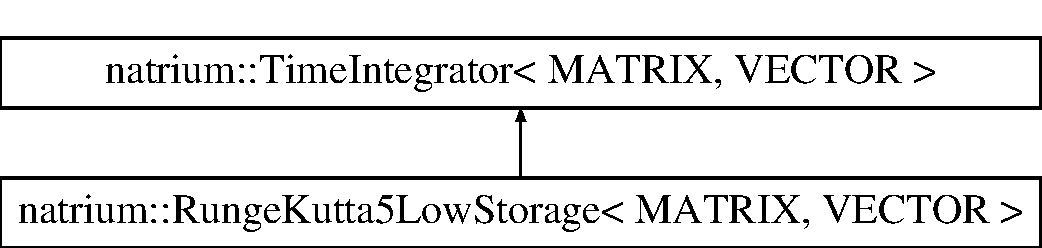
\includegraphics[height=2.000000cm]{classnatrium_1_1RungeKutta5LowStorage}
\end{center}
\end{figure}
\subsection*{\-Public \-Member \-Functions}
\begin{DoxyCompactItemize}
\item 
\hypertarget{classnatrium_1_1RungeKutta5LowStorage_adcb00ef16369158a395ecb54e5d5f91e}{\hyperlink{classnatrium_1_1RungeKutta5LowStorage_adcb00ef16369158a395ecb54e5d5f91e}{\-Runge\-Kutta5\-Low\-Storage} ()}\label{classnatrium_1_1RungeKutta5LowStorage_adcb00ef16369158a395ecb54e5d5f91e}

\begin{DoxyCompactList}\small\item\em constructor \end{DoxyCompactList}\item 
\hypertarget{classnatrium_1_1RungeKutta5LowStorage_a0d0e4591d2b671f450029bb3ba3053de}{virtual \hyperlink{classnatrium_1_1RungeKutta5LowStorage_a0d0e4591d2b671f450029bb3ba3053de}{$\sim$\-Runge\-Kutta5\-Low\-Storage} ()}\label{classnatrium_1_1RungeKutta5LowStorage_a0d0e4591d2b671f450029bb3ba3053de}

\begin{DoxyCompactList}\small\item\em destructor \end{DoxyCompactList}\end{DoxyCompactItemize}


\subsection{\-Detailed \-Description}
\-Implementation of the fifth-\/order \-Runge-\/\-Kutta time integration scheme with low storage consumption. 

\begin{DoxyNote}{\-Note}
\-The scheme is described in \-Min and \-Lee (2011)\-: \-A spectral-\/element discontinuous \-Galerkin lattice \-Boltzmann method for nearly incompressible flows, \-J\-C\-P 230 pp. 245-\/259. 
\end{DoxyNote}


\-The documentation for this class was generated from the following files\-:\begin{DoxyCompactItemize}
\item 
/home/kraemer/eclipse\-\_\-workspace/\-N\-A\-Triu\-M/src/timeintegration/\hyperlink{RungeKutta5LowStorage_8h}{\-Runge\-Kutta5\-Low\-Storage.\-h}\item 
/home/kraemer/eclipse\-\_\-workspace/\-N\-A\-Triu\-M/src/timeintegration/\hyperlink{RungeKutta5LowStorage_8cpp}{\-Runge\-Kutta5\-Low\-Storage.\-cpp}\end{DoxyCompactItemize}

\hypertarget{classnatrium_1_1SimpleProblemDescription2D}{\section{natrium\-:\-:\-Simple\-Problem\-Description2\-D \-Class \-Reference}
\label{classnatrium_1_1SimpleProblemDescription2D}\index{natrium\-::\-Simple\-Problem\-Description2\-D@{natrium\-::\-Simple\-Problem\-Description2\-D}}
}


\-Description of simple 2\-D test problems, using boundary \-I\-Ds and easy-\/to-\/use boundary functions.  




{\ttfamily \#include $<$\-Simple\-Problem\-Description2\-D.\-h$>$}

\-Inheritance diagram for natrium\-:\-:\-Simple\-Problem\-Description2\-D\-:\begin{figure}[H]
\begin{center}
\leavevmode
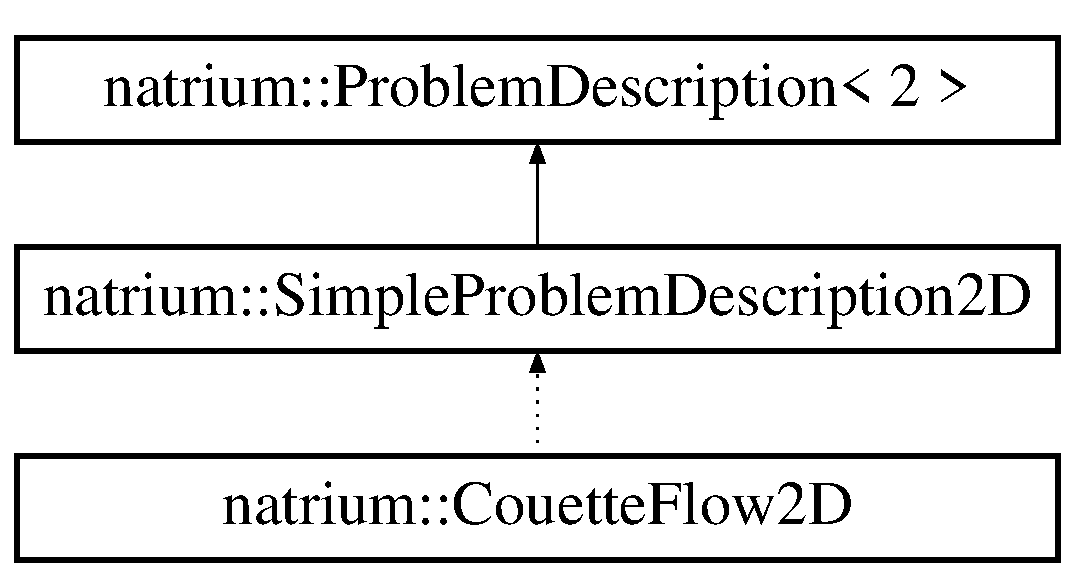
\includegraphics[height=3.000000cm]{classnatrium_1_1SimpleProblemDescription2D}
\end{center}
\end{figure}
\subsection*{\-Public \-Member \-Functions}
\begin{DoxyCompactItemize}
\item 
\hypertarget{classnatrium_1_1SimpleProblemDescription2D_a8b9dbf9876673e9b03bc4fa4a95036b4}{\hyperlink{classnatrium_1_1SimpleProblemDescription2D_a8b9dbf9876673e9b03bc4fa4a95036b4}{\-Simple\-Problem\-Description2\-D} ()}\label{classnatrium_1_1SimpleProblemDescription2D_a8b9dbf9876673e9b03bc4fa4a95036b4}

\begin{DoxyCompactList}\small\item\em constructor \end{DoxyCompactList}\item 
\hypertarget{classnatrium_1_1SimpleProblemDescription2D_a350cd6fd7ee17aed498659d51088e3e1}{virtual \hyperlink{classnatrium_1_1SimpleProblemDescription2D_a350cd6fd7ee17aed498659d51088e3e1}{$\sim$\-Simple\-Problem\-Description2\-D} ()}\label{classnatrium_1_1SimpleProblemDescription2D_a350cd6fd7ee17aed498659d51088e3e1}

\begin{DoxyCompactList}\small\item\em destructor \end{DoxyCompactList}\end{DoxyCompactItemize}


\subsection{\-Detailed \-Description}
\-Description of simple 2\-D test problems, using boundary \-I\-Ds and easy-\/to-\/use boundary functions. 

\-The documentation for this class was generated from the following files\-:\begin{DoxyCompactItemize}
\item 
/home/kraemer/eclipse\-\_\-workspace/\-N\-A\-Triu\-M/src/problemdescription/\hyperlink{SimpleProblemDescription2D_8h}{\-Simple\-Problem\-Description2\-D.\-h}\item 
/home/kraemer/eclipse\-\_\-workspace/\-N\-A\-Triu\-M/src/problemdescription/\hyperlink{SimpleProblemDescription2D_8cpp}{\-Simple\-Problem\-Description2\-D.\-cpp}\end{DoxyCompactItemize}

\hypertarget{classnatrium_1_1SolverConfiguration}{
\section{natrium::SolverConfiguration Class Reference}
\label{classnatrium_1_1SolverConfiguration}\index{natrium::SolverConfiguration@{natrium::SolverConfiguration}}
}


Class that stores the configuration for a CFD simulation based on the Discrete Boltzmann Equation (DBE).  


{\ttfamily \#include $<$SolverConfiguration.h$>$}\subsection*{Public Member Functions}
\begin{DoxyCompactItemize}
\item 
\hypertarget{classnatrium_1_1SolverConfiguration_a9aa7109e2eac9b8a7b424a35509ccdb0}{
\hyperlink{classnatrium_1_1SolverConfiguration_a9aa7109e2eac9b8a7b424a35509ccdb0}{SolverConfiguration} ()}
\label{classnatrium_1_1SolverConfiguration_a9aa7109e2eac9b8a7b424a35509ccdb0}

\begin{DoxyCompactList}\small\item\em Constructor -\/-\/ initializes parameters with their default values. \item\end{DoxyCompactList}\item 
\hyperlink{classnatrium_1_1SolverConfiguration_a062fa86eca607f830540ef4f2c06f0b3}{SolverConfiguration} (const std::string \&XMLfilename)
\begin{DoxyCompactList}\small\item\em Constructor -\/-\/ initializes parameters from an xmlfile. \item\end{DoxyCompactList}\item 
\hypertarget{classnatrium_1_1SolverConfiguration_ac1b521d8c205b8774dbb7c038304336d}{
virtual \hyperlink{classnatrium_1_1SolverConfiguration_ac1b521d8c205b8774dbb7c038304336d}{$\sim$SolverConfiguration} ()}
\label{classnatrium_1_1SolverConfiguration_ac1b521d8c205b8774dbb7c038304336d}

\begin{DoxyCompactList}\small\item\em destructor \item\end{DoxyCompactList}\item 
\hypertarget{classnatrium_1_1SolverConfiguration_a03f1592b0ef8c53729c5bbb9b17e5eb4}{
void \hyperlink{classnatrium_1_1SolverConfiguration_a03f1592b0ef8c53729c5bbb9b17e5eb4}{readFromTextFile} (const std::string \&filename, const bool optional=true, const bool write\_\-stripped\_\-file=false)}
\label{classnatrium_1_1SolverConfiguration_a03f1592b0ef8c53729c5bbb9b17e5eb4}

\begin{DoxyCompactList}\small\item\em wrapper function for ParameterHandler::read\_\-input; directing cerr into a C++-\/Exception \item\end{DoxyCompactList}\item 
\hypertarget{classnatrium_1_1SolverConfiguration_a18c63509007270fa96212fef36a2c172}{
void \hyperlink{classnatrium_1_1SolverConfiguration_a18c63509007270fa96212fef36a2c172}{readFromXMLFile} (const std::string \&filename)}
\label{classnatrium_1_1SolverConfiguration_a18c63509007270fa96212fef36a2c172}

\begin{DoxyCompactList}\small\item\em wrapper function for ParameterHandler::read\_\-input\_\-from\_\-xml; directing cerr into a C++-\/Exception \item\end{DoxyCompactList}\item 
\hypertarget{classnatrium_1_1SolverConfiguration_a90f8fb87f504897d3bbbc746749d2967}{
void \hyperlink{classnatrium_1_1SolverConfiguration_a90f8fb87f504897d3bbbc746749d2967}{isConsistent} ()}
\label{classnatrium_1_1SolverConfiguration_a90f8fb87f504897d3bbbc746749d2967}

\begin{DoxyCompactList}\small\item\em Check if the configuration is consistent. \item\end{DoxyCompactList}\item 
void \hyperlink{classnatrium_1_1SolverConfiguration_a69c009fd87690677b66ab10a000d07f6}{prepareOutputDirectory} ()
\begin{DoxyCompactList}\small\item\em prepare the Output directory \item\end{DoxyCompactList}\item 
void \hyperlink{classnatrium_1_1SolverConfiguration_a368a252965c1b23f7ad6811fdd0adcd4}{checkProblem} (boost::shared\_\-ptr$<$ \hyperlink{classnatrium_1_1ProblemDescription}{ProblemDescription}$<$ 2 $>$ $>$)
\begin{DoxyCompactList}\small\item\em Check if the problem definition is in accordance with the solver configuration. \item\end{DoxyCompactList}\item 
void \hyperlink{classnatrium_1_1SolverConfiguration_a3c66c7b0c5de2bee900835931c50ed5a}{checkProblem} (boost::shared\_\-ptr$<$ \hyperlink{classnatrium_1_1ProblemDescription}{ProblemDescription}$<$ 3 $>$ $>$)
\begin{DoxyCompactList}\small\item\em Check if the problem definition is in accordance with the solver configuration. \item\end{DoxyCompactList}\item 
\hypertarget{classnatrium_1_1SolverConfiguration_aaf32180358f99d78d56b3435dff11a11}{
AdvectionSchemeName {\bfseries getAdvectionScheme} ()}
\label{classnatrium_1_1SolverConfiguration_aaf32180358f99d78d56b3435dff11a11}

\item 
\hypertarget{classnatrium_1_1SolverConfiguration_a4fef165cd5a17247203af08846ec0f31}{
void {\bfseries setAdvectionScheme} (AdvectionSchemeName advectionScheme)}
\label{classnatrium_1_1SolverConfiguration_a4fef165cd5a17247203af08846ec0f31}

\item 
\hypertarget{classnatrium_1_1SolverConfiguration_a90e61c6fa9387a1cbf5943674bf307a8}{
CollisionSchemeName {\bfseries getCollisionScheme} ()}
\label{classnatrium_1_1SolverConfiguration_a90e61c6fa9387a1cbf5943674bf307a8}

\item 
\hypertarget{classnatrium_1_1SolverConfiguration_a5e7241337aa70cbe4b8af29c9cb5cfe8}{
void {\bfseries setCollisionScheme} (CollisionSchemeName collisionScheme)}
\label{classnatrium_1_1SolverConfiguration_a5e7241337aa70cbe4b8af29c9cb5cfe8}

\item 
\hypertarget{classnatrium_1_1SolverConfiguration_a4ebcfcb30f5cb6efb0d9fb3978b9b90f}{
double {\bfseries getBGKSteadyStateGamma} ()}
\label{classnatrium_1_1SolverConfiguration_a4ebcfcb30f5cb6efb0d9fb3978b9b90f}

\item 
\hypertarget{classnatrium_1_1SolverConfiguration_a040a4e68a3ce9502e39deb343586d62b}{
void {\bfseries setBGKSteadyStateGamma} (double gamma)}
\label{classnatrium_1_1SolverConfiguration_a040a4e68a3ce9502e39deb343586d62b}

\item 
\hypertarget{classnatrium_1_1SolverConfiguration_ac1954ee6d225807f947222c437fcd6a4}{
size\_\-t {\bfseries getCommandLineVerbosity} ()}
\label{classnatrium_1_1SolverConfiguration_ac1954ee6d225807f947222c437fcd6a4}

\item 
\hypertarget{classnatrium_1_1SolverConfiguration_a906afb09b544bf2137c0d3bf9214b4a5}{
void {\bfseries setCommandLineVerbosity} (long int commandLineVerbosity)}
\label{classnatrium_1_1SolverConfiguration_a906afb09b544bf2137c0d3bf9214b4a5}

\item 
\hypertarget{classnatrium_1_1SolverConfiguration_a43270017646e2efa400ae84d644ac897}{
bool {\bfseries hasAnalyticSolution} ()}
\label{classnatrium_1_1SolverConfiguration_a43270017646e2efa400ae84d644ac897}

\item 
\hypertarget{classnatrium_1_1SolverConfiguration_ae23ef2513c7b4ed3eacd678e38ff146f}{
void {\bfseries setHasAnalyticSolution} (bool hasAnalyticSolution)}
\label{classnatrium_1_1SolverConfiguration_ae23ef2513c7b4ed3eacd678e38ff146f}

\item 
\hypertarget{classnatrium_1_1SolverConfiguration_afe9fd2087df0ab6066f260bf6bfd03ac}{
InitializationSchemeName {\bfseries getInitializationScheme} ()}
\label{classnatrium_1_1SolverConfiguration_afe9fd2087df0ab6066f260bf6bfd03ac}

\item 
\hypertarget{classnatrium_1_1SolverConfiguration_a4d867b8b8c0c08fc68b95f1a1a52c95d}{
void {\bfseries setInitializationScheme} (InitializationSchemeName initializationScheme)}
\label{classnatrium_1_1SolverConfiguration_a4d867b8b8c0c08fc68b95f1a1a52c95d}

\item 
\hypertarget{classnatrium_1_1SolverConfiguration_aa12123336ffa7489780baa45d99569b1}{
size\_\-t {\bfseries getIterativeInitializationNumberOfIterations} ()}
\label{classnatrium_1_1SolverConfiguration_aa12123336ffa7489780baa45d99569b1}

\item 
\hypertarget{classnatrium_1_1SolverConfiguration_ac4188dce03b129130f153f7028c3f79e}{
void {\bfseries setIterativeInitializationNumberOfIterations} (long int iterativeInitializationNumberOfIterations)}
\label{classnatrium_1_1SolverConfiguration_ac4188dce03b129130f153f7028c3f79e}

\item 
\hypertarget{classnatrium_1_1SolverConfiguration_a966eee9da52af6fbd1f8d5fad2b8427a}{
double {\bfseries getIterativeInitializationResidual} ()}
\label{classnatrium_1_1SolverConfiguration_a966eee9da52af6fbd1f8d5fad2b8427a}

\item 
\hypertarget{classnatrium_1_1SolverConfiguration_ad9551932a38bda46c8ca2ef88a73e754}{
void {\bfseries setIterativeInitializationResidual} (double iterativeInitializationResidual)}
\label{classnatrium_1_1SolverConfiguration_ad9551932a38bda46c8ca2ef88a73e754}

\item 
\hypertarget{classnatrium_1_1SolverConfiguration_a13121a202636553339d5b1f83d196fd7}{
size\_\-t {\bfseries getNumberOfTimeSteps} ()}
\label{classnatrium_1_1SolverConfiguration_a13121a202636553339d5b1f83d196fd7}

\item 
\hypertarget{classnatrium_1_1SolverConfiguration_a50c43893f5c6ed0d73fcccd64f523053}{
void {\bfseries setNumberOfTimeSteps} (long int numberOfTimeSteps)}
\label{classnatrium_1_1SolverConfiguration_a50c43893f5c6ed0d73fcccd64f523053}

\item 
\hypertarget{classnatrium_1_1SolverConfiguration_aa0d9cd3a8d2e6e04fc33e3b4fb8785d9}{
double {\bfseries getSimulationEndTime} ()}
\label{classnatrium_1_1SolverConfiguration_aa0d9cd3a8d2e6e04fc33e3b4fb8785d9}

\item 
\hypertarget{classnatrium_1_1SolverConfiguration_a0d64bd79313ae1aa022d9a2c0e6bc3fd}{
void {\bfseries setSimulationEndTime} (double end\_\-time)}
\label{classnatrium_1_1SolverConfiguration_a0d64bd79313ae1aa022d9a2c0e6bc3fd}

\item 
\hypertarget{classnatrium_1_1SolverConfiguration_a221b5a32cb4cc871536f68a26e14b3c8}{
double {\bfseries getConvergenceThreshold} ()}
\label{classnatrium_1_1SolverConfiguration_a221b5a32cb4cc871536f68a26e14b3c8}

\item 
\hypertarget{classnatrium_1_1SolverConfiguration_a8e7af89ae281933e0f70771ef09147b0}{
void {\bfseries setConvergenceThreshold} (double threshold)}
\label{classnatrium_1_1SolverConfiguration_a8e7af89ae281933e0f70771ef09147b0}

\item 
\hypertarget{classnatrium_1_1SolverConfiguration_a7b7ffc9156ba827ab74ff6f1d7bd9151}{
size\_\-t {\bfseries getOutputCheckpointInterval} ()}
\label{classnatrium_1_1SolverConfiguration_a7b7ffc9156ba827ab74ff6f1d7bd9151}

\item 
\hypertarget{classnatrium_1_1SolverConfiguration_ab7a39dfb46cb1b0c7b54b92700fd7360}{
void {\bfseries setOutputCheckpointInterval} (long int outputCheckpointInterval)}
\label{classnatrium_1_1SolverConfiguration_ab7a39dfb46cb1b0c7b54b92700fd7360}

\item 
\hypertarget{classnatrium_1_1SolverConfiguration_a6c0fb63902a6828c06c48918402375bb}{
size\_\-t {\bfseries getOutputTableInterval} ()}
\label{classnatrium_1_1SolverConfiguration_a6c0fb63902a6828c06c48918402375bb}

\item 
\hypertarget{classnatrium_1_1SolverConfiguration_a207c38e009015be45e74eaa86f9db7ad}{
void {\bfseries setOutputTableInterval} (long int outputTableInterval)}
\label{classnatrium_1_1SolverConfiguration_a207c38e009015be45e74eaa86f9db7ad}

\item 
\hypertarget{classnatrium_1_1SolverConfiguration_a2a0444878a5fb512772e024bc03ec076}{
const std::string {\bfseries getOutputDirectory} ()}
\label{classnatrium_1_1SolverConfiguration_a2a0444878a5fb512772e024bc03ec076}

\item 
\hypertarget{classnatrium_1_1SolverConfiguration_acd249488bb83773514c4d6917b5bfc3a}{
void {\bfseries setOutputDirectory} (const std::string \&outputDirectory)}
\label{classnatrium_1_1SolverConfiguration_acd249488bb83773514c4d6917b5bfc3a}

\item 
\hypertarget{classnatrium_1_1SolverConfiguration_aa7fdb1358469be8faf1cc14c64538927}{
size\_\-t {\bfseries getOutputSolutionInterval} ()}
\label{classnatrium_1_1SolverConfiguration_aa7fdb1358469be8faf1cc14c64538927}

\item 
\hypertarget{classnatrium_1_1SolverConfiguration_ab49c72f19d58f7408eb14ac7fd865b78}{
void {\bfseries setOutputSolutionInterval} (long int outputSolutionInterval)}
\label{classnatrium_1_1SolverConfiguration_ab49c72f19d58f7408eb14ac7fd865b78}

\item 
\hypertarget{classnatrium_1_1SolverConfiguration_a6ca256e404b94f7201ecace9307ef1df}{
bool {\bfseries isRestartAtLastCheckpoint} ()}
\label{classnatrium_1_1SolverConfiguration_a6ca256e404b94f7201ecace9307ef1df}

\item 
\hypertarget{classnatrium_1_1SolverConfiguration_af6077ef11412e53eb16c013b4362410e}{
void {\bfseries setRestartAtLastCheckpoint} (bool restartAtLastCheckpoint)}
\label{classnatrium_1_1SolverConfiguration_af6077ef11412e53eb16c013b4362410e}

\item 
\hypertarget{classnatrium_1_1SolverConfiguration_aecc2a87bc6e50d6e09ea035678478c4f}{
FluxTypeName {\bfseries getSedgFluxType} ()}
\label{classnatrium_1_1SolverConfiguration_aecc2a87bc6e50d6e09ea035678478c4f}

\item 
\hypertarget{classnatrium_1_1SolverConfiguration_a331256f91794e32be618b1162c321bdd}{
void {\bfseries setSedgFluxType} (FluxTypeName sedgFluxType)}
\label{classnatrium_1_1SolverConfiguration_a331256f91794e32be618b1162c321bdd}

\item 
\hypertarget{classnatrium_1_1SolverConfiguration_a1fad5bbbc062b1aad018da73e90033b2}{
size\_\-t {\bfseries getSedgOrderOfFiniteElement} ()}
\label{classnatrium_1_1SolverConfiguration_a1fad5bbbc062b1aad018da73e90033b2}

\item 
\hypertarget{classnatrium_1_1SolverConfiguration_a2a9ab8b6b6dcb47ad4bb85ef06e15dea}{
void {\bfseries setSedgOrderOfFiniteElement} (long int sedgOrderOfFiniteElement)}
\label{classnatrium_1_1SolverConfiguration_a2a9ab8b6b6dcb47ad4bb85ef06e15dea}

\item 
\hypertarget{classnatrium_1_1SolverConfiguration_adb7b45c43f97f0ce2ca288f92a32b577}{
double {\bfseries getStencilScaling} ()}
\label{classnatrium_1_1SolverConfiguration_adb7b45c43f97f0ce2ca288f92a32b577}

\item 
\hypertarget{classnatrium_1_1SolverConfiguration_a1dff19c0a3cc7386bd629dd72e59ac42}{
void {\bfseries setStencilScaling} (double stencilScaling)}
\label{classnatrium_1_1SolverConfiguration_a1dff19c0a3cc7386bd629dd72e59ac42}

\item 
\hypertarget{classnatrium_1_1SolverConfiguration_a962af94c9599c393d8a16d7f5ae04d6c}{
StencilType {\bfseries getStencil} ()}
\label{classnatrium_1_1SolverConfiguration_a962af94c9599c393d8a16d7f5ae04d6c}

\item 
\hypertarget{classnatrium_1_1SolverConfiguration_afa50192447fb027d0250a29b1ea86d1a}{
void {\bfseries setStencil} (StencilType stencil)}
\label{classnatrium_1_1SolverConfiguration_afa50192447fb027d0250a29b1ea86d1a}

\item 
\hypertarget{classnatrium_1_1SolverConfiguration_ac7e6189aaa1b54016993e852999376eb}{
TimeIntegratorName {\bfseries getTimeIntegrator} ()}
\label{classnatrium_1_1SolverConfiguration_ac7e6189aaa1b54016993e852999376eb}

\item 
\hypertarget{classnatrium_1_1SolverConfiguration_ac58399f50e64bc8b0efde5b51e246aeb}{
void {\bfseries setTimeIntegrator} (TimeIntegratorName timeIntegrator)}
\label{classnatrium_1_1SolverConfiguration_ac58399f50e64bc8b0efde5b51e246aeb}

\item 
\hypertarget{classnatrium_1_1SolverConfiguration_a0e2606b5c10964a08e7107dbe079a1ed}{
double {\bfseries getThetaMethodTheta} ()}
\label{classnatrium_1_1SolverConfiguration_a0e2606b5c10964a08e7107dbe079a1ed}

\item 
\hypertarget{classnatrium_1_1SolverConfiguration_acb2153b276dfc0e28bb2cabf8855acd0}{
void {\bfseries setThetaMethodTheta} (double theta)}
\label{classnatrium_1_1SolverConfiguration_acb2153b276dfc0e28bb2cabf8855acd0}

\item 
\hypertarget{classnatrium_1_1SolverConfiguration_a5ba156b86d81572776d8c20b04f21dcc}{
DealIntegratorName {\bfseries getDealIntegrator} ()}
\label{classnatrium_1_1SolverConfiguration_a5ba156b86d81572776d8c20b04f21dcc}

\item 
\hypertarget{classnatrium_1_1SolverConfiguration_acf54eacaa0135343d69a31f0bbc8031c}{
void {\bfseries setDealIntegrator} (DealIntegratorName integrator)}
\label{classnatrium_1_1SolverConfiguration_acf54eacaa0135343d69a31f0bbc8031c}

\item 
\hypertarget{classnatrium_1_1SolverConfiguration_a0678dd0f89508e37c5c555413d5dc258}{
DealSolverName {\bfseries getDealLinearSolver} ()}
\label{classnatrium_1_1SolverConfiguration_a0678dd0f89508e37c5c555413d5dc258}

\item 
\hypertarget{classnatrium_1_1SolverConfiguration_a63ab4a5ff44381dfff6558c030fa3665}{
void {\bfseries setDealLinearSolver} (DealSolverName solver)}
\label{classnatrium_1_1SolverConfiguration_a63ab4a5ff44381dfff6558c030fa3665}

\item 
\hypertarget{classnatrium_1_1SolverConfiguration_a7a017f7078ef42c350efbfca51d9681c}{
void {\bfseries setEmbeddedDealIntegratorParameters} (double coarsen\_\-param, double refine\_\-param, double min\_\-delta, double max\_\-delta, double refine\_\-tol, double coarsen\_\-tol)}
\label{classnatrium_1_1SolverConfiguration_a7a017f7078ef42c350efbfca51d9681c}

\item 
\hypertarget{classnatrium_1_1SolverConfiguration_a0e233c5ac8c6387bf31923700fd95b56}{
double {\bfseries getEmbeddedDealIntegratorCoarsenParameter} ()}
\label{classnatrium_1_1SolverConfiguration_a0e233c5ac8c6387bf31923700fd95b56}

\item 
\hypertarget{classnatrium_1_1SolverConfiguration_a9f8fda7b80e405dab21388cdb0eacbbe}{
double {\bfseries getEmbeddedDealIntegratorRefinementParameter} ()}
\label{classnatrium_1_1SolverConfiguration_a9f8fda7b80e405dab21388cdb0eacbbe}

\item 
\hypertarget{classnatrium_1_1SolverConfiguration_a42688d5882305d75929798685dcd3b0b}{
double {\bfseries getEmbeddedDealIntegratorMinimumTimeStep} ()}
\label{classnatrium_1_1SolverConfiguration_a42688d5882305d75929798685dcd3b0b}

\item 
\hypertarget{classnatrium_1_1SolverConfiguration_a01efc16a1f7c548ef83acdf4bb5bdaf4}{
double {\bfseries getEmbeddedDealIntegratorMaximumTimeStep} ()}
\label{classnatrium_1_1SolverConfiguration_a01efc16a1f7c548ef83acdf4bb5bdaf4}

\item 
\hypertarget{classnatrium_1_1SolverConfiguration_a2c6da5cc4bcfc653c0f3b93b57a4ddf5}{
double {\bfseries getEmbeddedDealIntegratorRefinementTolerance} ()}
\label{classnatrium_1_1SolverConfiguration_a2c6da5cc4bcfc653c0f3b93b57a4ddf5}

\item 
\hypertarget{classnatrium_1_1SolverConfiguration_afedfb3328b78940a7e929214c6d08741}{
double {\bfseries getEmbeddedDealIntegratorCoarsenTolerance} ()}
\label{classnatrium_1_1SolverConfiguration_afedfb3328b78940a7e929214c6d08741}

\item 
\hypertarget{classnatrium_1_1SolverConfiguration_ae446f5d60a09f30a43258a5ec2bebbbf}{
double {\bfseries getTimeStepSize} ()}
\label{classnatrium_1_1SolverConfiguration_ae446f5d60a09f30a43258a5ec2bebbbf}

\item 
\hypertarget{classnatrium_1_1SolverConfiguration_aab0d1b737708c92e83ebe3424b3bed4d}{
void {\bfseries setTimeStepSize} (double timeStepSize)}
\label{classnatrium_1_1SolverConfiguration_aab0d1b737708c92e83ebe3424b3bed4d}

\item 
\hypertarget{classnatrium_1_1SolverConfiguration_ac97dc43684f8a690de0f3e9c132dda02}{
bool {\bfseries isWriteALogFile} ()}
\label{classnatrium_1_1SolverConfiguration_ac97dc43684f8a690de0f3e9c132dda02}

\item 
\hypertarget{classnatrium_1_1SolverConfiguration_a6e50f8fc372b4346ba9f309d5d5f47b3}{
void {\bfseries setWriteALogFile} (bool writeALogFile)}
\label{classnatrium_1_1SolverConfiguration_a6e50f8fc372b4346ba9f309d5d5f47b3}

\item 
\hypertarget{classnatrium_1_1SolverConfiguration_ae4852378b026ccc913732eb8b20eca74}{
bool {\bfseries isSwitchOutputOff} ()}
\label{classnatrium_1_1SolverConfiguration_ae4852378b026ccc913732eb8b20eca74}

\item 
\hypertarget{classnatrium_1_1SolverConfiguration_afcae7f43456c2a127c242b230ea3a8a2}{
void {\bfseries setSwitchOutputOff} (bool switchOutputOff)}
\label{classnatrium_1_1SolverConfiguration_afcae7f43456c2a127c242b230ea3a8a2}

\item 
\hypertarget{classnatrium_1_1SolverConfiguration_a6e41f8ce5da4ecafe2e4326997e79f3d}{
bool {\bfseries isUserInteraction} ()}
\label{classnatrium_1_1SolverConfiguration_a6e41f8ce5da4ecafe2e4326997e79f3d}

\item 
\hypertarget{classnatrium_1_1SolverConfiguration_ad013b9240ee7ae0d5cc43ff5f588c3f3}{
void {\bfseries setUserInteraction} (bool userInteract)}
\label{classnatrium_1_1SolverConfiguration_ad013b9240ee7ae0d5cc43ff5f588c3f3}

\end{DoxyCompactItemize}


\subsection{Detailed Description}
Class that stores the configuration for a CFD simulation based on the Discrete Boltzmann Equation (DBE). \begin{DoxyNote}{Note}
The class is a subclass of dealii::ParameterHandler and functions as a wrapper. 

To integrate new parameter into the framework, you have to declare the paramters in the constructor and write the getter and setter. The setter and getter have to navigate through the sections of the Parameter handler and catch the exceptions thrown by the Parameter handler. Finally you have to update the preprocessor/NATriuM\_\-parameters.xml file, most easily run the UnitTests and copy results/NATriuM\_\-parameters.xml there. The latter file is automatically created according to the declared parameters. Every selection-\/type parameter (e.g. Advection scheme) is implemented as an enum for better handling through the command line. 
\end{DoxyNote}
\begin{Desc}
\item[Examples: ]\par


\hyperlink{step-0_8cpp-example}{step-\/0.cpp}.\end{Desc}


\subsection{Constructor \& Destructor Documentation}
\hypertarget{classnatrium_1_1SolverConfiguration_a062fa86eca607f830540ef4f2c06f0b3}{
\index{natrium::SolverConfiguration@{natrium::SolverConfiguration}!SolverConfiguration@{SolverConfiguration}}
\index{SolverConfiguration@{SolverConfiguration}!natrium::SolverConfiguration@{natrium::SolverConfiguration}}
\subsubsection[{SolverConfiguration}]{\setlength{\rightskip}{0pt plus 5cm}natrium::SolverConfiguration::SolverConfiguration (const std::string \& {\em XMLfilename})}}
\label{classnatrium_1_1SolverConfiguration_a062fa86eca607f830540ef4f2c06f0b3}


Constructor -\/-\/ initializes parameters from an xmlfile. 
\begin{DoxyExceptions}{Exceptions}
\item[{\em \hyperlink{classnatrium_1_1ConfigurationException}{ConfigurationException}}]if the XML file has wrong format \end{DoxyExceptions}


\subsection{Member Function Documentation}
\hypertarget{classnatrium_1_1SolverConfiguration_a3c66c7b0c5de2bee900835931c50ed5a}{
\index{natrium::SolverConfiguration@{natrium::SolverConfiguration}!checkProblem@{checkProblem}}
\index{checkProblem@{checkProblem}!natrium::SolverConfiguration@{natrium::SolverConfiguration}}
\subsubsection[{checkProblem}]{\setlength{\rightskip}{0pt plus 5cm}void natrium::SolverConfiguration::checkProblem (boost::shared\_\-ptr$<$ {\bf ProblemDescription}$<$ 3 $>$ $>$)\hspace{0.3cm}{\ttfamily  \mbox{[}inline\mbox{]}}}}
\label{classnatrium_1_1SolverConfiguration_a3c66c7b0c5de2bee900835931c50ed5a}


Check if the problem definition is in accordance with the solver configuration. 
\begin{DoxyParams}{Parameters}
\item[\mbox{$\leftarrow$} {\em cFDProblem}]Shared pointer to a problem description\end{DoxyParams}

\begin{DoxyExceptions}{Exceptions}
\item[{\em ...}]//TODO implement custom exception \end{DoxyExceptions}
\hypertarget{classnatrium_1_1SolverConfiguration_a368a252965c1b23f7ad6811fdd0adcd4}{
\index{natrium::SolverConfiguration@{natrium::SolverConfiguration}!checkProblem@{checkProblem}}
\index{checkProblem@{checkProblem}!natrium::SolverConfiguration@{natrium::SolverConfiguration}}
\subsubsection[{checkProblem}]{\setlength{\rightskip}{0pt plus 5cm}void natrium::SolverConfiguration::checkProblem (boost::shared\_\-ptr$<$ {\bf ProblemDescription}$<$ 2 $>$ $>$)\hspace{0.3cm}{\ttfamily  \mbox{[}inline\mbox{]}}}}
\label{classnatrium_1_1SolverConfiguration_a368a252965c1b23f7ad6811fdd0adcd4}


Check if the problem definition is in accordance with the solver configuration. 
\begin{DoxyParams}{Parameters}
\item[\mbox{$\leftarrow$} {\em cFDProblem}]Shared pointer to a problem description\end{DoxyParams}

\begin{DoxyExceptions}{Exceptions}
\item[{\em ...}]//TODO implement custom exception \end{DoxyExceptions}
\hypertarget{classnatrium_1_1SolverConfiguration_a69c009fd87690677b66ab10a000d07f6}{
\index{natrium::SolverConfiguration@{natrium::SolverConfiguration}!prepareOutputDirectory@{prepareOutputDirectory}}
\index{prepareOutputDirectory@{prepareOutputDirectory}!natrium::SolverConfiguration@{natrium::SolverConfiguration}}
\subsubsection[{prepareOutputDirectory}]{\setlength{\rightskip}{0pt plus 5cm}void natrium::SolverConfiguration::prepareOutputDirectory ()}}
\label{classnatrium_1_1SolverConfiguration_a69c009fd87690677b66ab10a000d07f6}


prepare the Output directory \begin{DoxyNote}{Note}
If 'User interaction' is enabled, user input is requested in case of possible overwriting 
\end{DoxyNote}

\begin{DoxyExceptions}{Exceptions}
\item[{\em SolverConfigurationError,if}]it was not possible \end{DoxyExceptions}


If not exists, try to create output directory

try to open all files

try to create a single file 

The documentation for this class was generated from the following files:\begin{DoxyCompactItemize}
\item 
/mnt/fdrive/akraem3m/workspace/NATriuM/src/library/natrium/solver/\hyperlink{SolverConfiguration_8h}{SolverConfiguration.h}\item 
/mnt/fdrive/akraem3m/workspace/NATriuM/src/library/natrium/solver/\hyperlink{SolverConfiguration_8cpp}{SolverConfiguration.cpp}\end{DoxyCompactItemize}

\hypertarget{classnatrium_1_1StreamingData}{\section{natrium\-:\-:\-Streaming\-Data$<$ dim $>$ \-Class \-Template \-Reference}
\label{classnatrium_1_1StreamingData}\index{natrium\-::\-Streaming\-Data$<$ dim $>$@{natrium\-::\-Streaming\-Data$<$ dim $>$}}
}


\-Abstract class to store global streaming data, like e.\-g. the particle distributions.  




{\ttfamily \#include $<$\-Streaming\-Data.\-h$>$}

\-Inheritance diagram for natrium\-:\-:\-Streaming\-Data$<$ dim $>$\-:\begin{figure}[H]
\begin{center}
\leavevmode
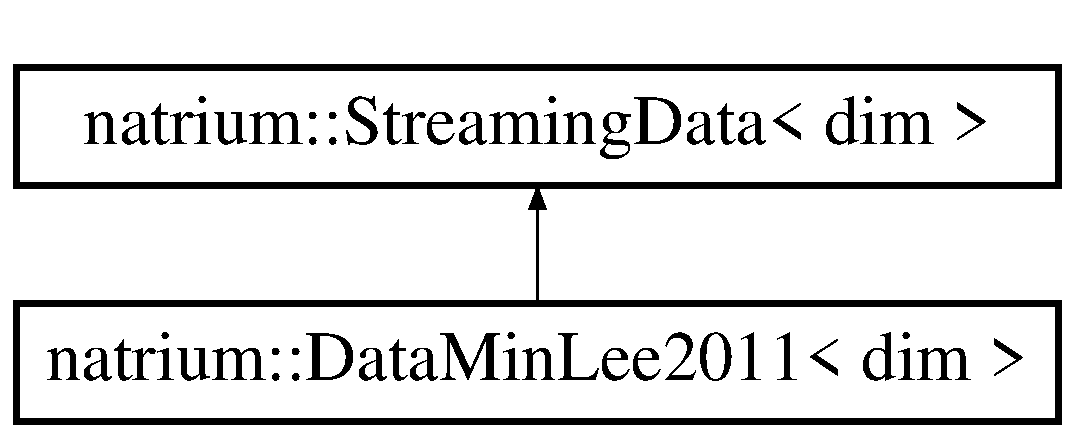
\includegraphics[height=2.000000cm]{classnatrium_1_1StreamingData}
\end{center}
\end{figure}
\subsection*{\-Public \-Member \-Functions}
\begin{DoxyCompactItemize}
\item 
\hypertarget{classnatrium_1_1StreamingData_a176886d4ba1765194fe675775a2f6087}{\hyperlink{classnatrium_1_1StreamingData_a176886d4ba1765194fe675775a2f6087}{\-Streaming\-Data} ()}\label{classnatrium_1_1StreamingData_a176886d4ba1765194fe675775a2f6087}

\begin{DoxyCompactList}\small\item\em constructor \end{DoxyCompactList}\item 
\hypertarget{classnatrium_1_1StreamingData_a11f35edbebcb05646e034f6a918cf7c7}{virtual \hyperlink{classnatrium_1_1StreamingData_a11f35edbebcb05646e034f6a918cf7c7}{$\sim$\-Streaming\-Data} ()}\label{classnatrium_1_1StreamingData_a11f35edbebcb05646e034f6a918cf7c7}

\begin{DoxyCompactList}\small\item\em destructor \end{DoxyCompactList}\end{DoxyCompactItemize}


\subsection{\-Detailed \-Description}
\subsubsection*{template$<$int dim$>$class natrium\-::\-Streaming\-Data$<$ dim $>$}

\-Abstract class to store global streaming data, like e.\-g. the particle distributions. 

\begin{DoxyNote}{\-Note}
\-The data to store differs for different approaches of solving the \-D\-B\-E. \-The only common data which will appear in every method is the particle distribution functions and some global system matrix. 
\end{DoxyNote}

\begin{DoxyTemplParams}{\-Template Parameters}
{\em dim} & \-The dimension of the flow (2 or 3). \\
\hline
\end{DoxyTemplParams}


\-The documentation for this class was generated from the following file\-:\begin{DoxyCompactItemize}
\item 
/home/kraemer/eclipse\-\_\-workspace/\-N\-A\-Triu\-M/src/streamingdata/\hyperlink{StreamingData_8h}{\-Streaming\-Data.\-h}\end{DoxyCompactItemize}

\hypertarget{classnatrium_1_1TimeIntegrator}{\section{natrium\-:\-:Time\-Integrator$<$ M\-A\-T\-R\-I\-X, V\-E\-C\-T\-O\-R $>$ Class Template Reference}
\label{classnatrium_1_1TimeIntegrator}\index{natrium\-::\-Time\-Integrator$<$ M\-A\-T\-R\-I\-X, V\-E\-C\-T\-O\-R $>$@{natrium\-::\-Time\-Integrator$<$ M\-A\-T\-R\-I\-X, V\-E\-C\-T\-O\-R $>$}}
}


Abstract class for time integration (solution of ordinary differential equations (O\-D\-E)).  




{\ttfamily \#include $<$Time\-Integrator.\-h$>$}

Inheritance diagram for natrium\-:\-:Time\-Integrator$<$ M\-A\-T\-R\-I\-X, V\-E\-C\-T\-O\-R $>$\-:\begin{figure}[H]
\begin{center}
\leavevmode
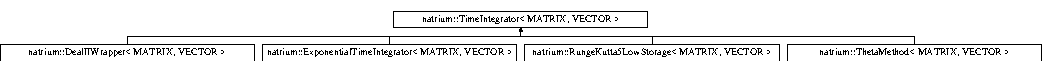
\includegraphics[height=1.666667cm]{classnatrium_1_1TimeIntegrator}
\end{center}
\end{figure}
\subsection*{Public Member Functions}
\begin{DoxyCompactItemize}
\item 
\hypertarget{classnatrium_1_1TimeIntegrator_a420ea9baabf0839bc8ecb5f5e02ce95b}{\hyperlink{classnatrium_1_1TimeIntegrator_a420ea9baabf0839bc8ecb5f5e02ce95b}{Time\-Integrator} (double time\-Step\-Size)}\label{classnatrium_1_1TimeIntegrator_a420ea9baabf0839bc8ecb5f5e02ce95b}

\begin{DoxyCompactList}\small\item\em constructor \end{DoxyCompactList}\item 
\hypertarget{classnatrium_1_1TimeIntegrator_a8795d06c5322b72a5a2a1f30aa7a051d}{virtual \hyperlink{classnatrium_1_1TimeIntegrator_a8795d06c5322b72a5a2a1f30aa7a051d}{$\sim$\-Time\-Integrator} ()}\label{classnatrium_1_1TimeIntegrator_a8795d06c5322b72a5a2a1f30aa7a051d}

\begin{DoxyCompactList}\small\item\em destructor \end{DoxyCompactList}\item 
\hypertarget{classnatrium_1_1TimeIntegrator_a6e763133e114cdd758307ca30b65f161}{double {\bfseries get\-Time\-Step\-Size} () const }\label{classnatrium_1_1TimeIntegrator_a6e763133e114cdd758307ca30b65f161}

\item 
\hypertarget{classnatrium_1_1TimeIntegrator_a18592866e946c63ab1595d3ab688ea6b}{void {\bfseries set\-Time\-Step\-Size} (double time\-Step\-Size)}\label{classnatrium_1_1TimeIntegrator_a18592866e946c63ab1595d3ab688ea6b}

\item 
\hypertarget{classnatrium_1_1TimeIntegrator_a09e1ad9254abec537cda42b1d2fb83e6}{virtual void \hyperlink{classnatrium_1_1TimeIntegrator_a09e1ad9254abec537cda42b1d2fb83e6}{step} (V\-E\-C\-T\-O\-R \&vector, const M\-A\-T\-R\-I\-X \&system\-Matrix, const V\-E\-C\-T\-O\-R \&system\-Vector)=0}\label{classnatrium_1_1TimeIntegrator_a09e1ad9254abec537cda42b1d2fb83e6}

\begin{DoxyCompactList}\small\item\em make one time integration step on vector using the system matrix \end{DoxyCompactList}\end{DoxyCompactItemize}


\subsection{Detailed Description}
\subsubsection*{template$<$class M\-A\-T\-R\-I\-X, class V\-E\-C\-T\-O\-R$>$class natrium\-::\-Time\-Integrator$<$ M\-A\-T\-R\-I\-X, V\-E\-C\-T\-O\-R $>$}

Abstract class for time integration (solution of ordinary differential equations (O\-D\-E)). 

\begin{DoxyNote}{Note}
The O\-D\-Es arise from the space discretization of the D\-B\-E, which is basically a partial differential equation (P\-D\-E). By application of a space discretization scheme (like discontinuous Galerkin or standard F\-E\-M methods) the space derivatives in the P\-D\-E are replaced with arithmetic expressions. The only remaining derivative is then the time derivative, which makes the equation an O\-D\-E. The latter can be solved using classical time integration methods like Runge-\/\-Kutta or Adams-\/\-Moulton. 
\end{DoxyNote}


The documentation for this class was generated from the following files\-:\begin{DoxyCompactItemize}
\item 
/home/kraemer/eclipse\-\_\-workspace/\-N\-A\-Triu\-M/src/natrium/timeintegration/\hyperlink{TimeIntegrator_8h}{Time\-Integrator.\-h}\item 
/home/kraemer/eclipse\-\_\-workspace/\-N\-A\-Triu\-M/src/natrium/timeintegration/\hyperlink{TimeIntegrator_8cpp}{Time\-Integrator.\-cpp}\end{DoxyCompactItemize}

\chapter{\-File \-Documentation}
\hypertarget{CouetteFlow2D_8cpp}{
\section{/mnt/fdrive/akraem3m/workspace/NATriuM/src/library/natrium/benchmarks/CouetteFlow2D.cpp File Reference}
\label{CouetteFlow2D_8cpp}\index{/mnt/fdrive/akraem3m/workspace/NATriuM/src/library/natrium/benchmarks/CouetteFlow2D.cpp@{/mnt/fdrive/akraem3m/workspace/NATriuM/src/library/natrium/benchmarks/CouetteFlow2D.cpp}}
}
{\ttfamily \#include \char`\"{}CouetteFlow2D.h\char`\"{}}\par
{\ttfamily \#include \char`\"{}deal.II/grid/grid\_\-generator.h\char`\"{}}\par
{\ttfamily \#include \char`\"{}deal.II/grid/grid\_\-tools.h\char`\"{}}\par
{\ttfamily \#include \char`\"{}deal.II/grid/grid\_\-out.h\char`\"{}}\par
{\ttfamily \#include \char`\"{}deal.II/grid/tria\_\-accessor.h\char`\"{}}\par
{\ttfamily \#include \char`\"{}deal.II/grid/tria\_\-iterator.h\char`\"{}}\par
{\ttfamily \#include \char`\"{}deal.II/base/geometry\_\-info.h\char`\"{}}\par
{\ttfamily \#include \char`\"{}../problemdescription/PeriodicBoundary.h\char`\"{}}\par
{\ttfamily \#include \char`\"{}../problemdescription/LinearBoundaryRhoU.h\char`\"{}}\par
{\ttfamily \#include \char`\"{}../utilities/Logging.h\char`\"{}}\par
{\ttfamily \#include \char`\"{}../utilities/MPIGuard.h\char`\"{}}\par


\subsection{Detailed Description}
\begin{DoxyDate}{Date}
29.05.2013 
\end{DoxyDate}
\begin{DoxyAuthor}{Author}
Andreas Kraemer, Bonn-\/Rhein-\/Sieg University of Applied Sciences, Sankt Augustin 
\end{DoxyAuthor}

\hypertarget{CouetteFlow2D_8h}{\section{/home/kraemer/eclipse\-\_\-workspace/\-N\-A\-Triu\-M/src/examples/step-\/3/\-Couette\-Flow2\-D.h File Reference}
\label{CouetteFlow2D_8h}\index{/home/kraemer/eclipse\-\_\-workspace/\-N\-A\-Triu\-M/src/examples/step-\/3/\-Couette\-Flow2\-D.\-h@{/home/kraemer/eclipse\-\_\-workspace/\-N\-A\-Triu\-M/src/examples/step-\/3/\-Couette\-Flow2\-D.\-h}}
}


Description of a simple Couette Flow (regular channel flow in rectangular domain).  


{\ttfamily \#include \char`\"{}deal.\-I\-I/grid/tria.\-h\char`\"{}}\\*
{\ttfamily \#include \char`\"{}problemdescription/\-Problem\-Description.\-h\char`\"{}}\\*
{\ttfamily \#include \char`\"{}utilities/\-Basic\-Names.\-h\char`\"{}}\\*
\subsection*{Classes}
\begin{DoxyCompactItemize}
\item 
class \hyperlink{classnatrium_1_1CouetteFlow2D}{natrium\-::\-Couette\-Flow2\-D}
\begin{DoxyCompactList}\small\item\em Description of a simple Couette Flow (regular channel flow in square domain). The domain is \mbox{[}0,1\mbox{]}$^\wedge$2. The top plate is moved with constant velocity. The domain consists of 8 x 8 = 64 Elements (contrast to Min and Lee, who have 6 x 6). \end{DoxyCompactList}\end{DoxyCompactItemize}


\subsection{Detailed Description}
Description of a simple Couette Flow (regular channel flow in rectangular domain). \begin{DoxyDate}{Date}
29.\-05.\-2013 
\end{DoxyDate}
\begin{DoxyAuthor}{Author}
Andreas Kraemer, Bonn-\/\-Rhein-\/\-Sieg University of Applied Sciences, Sankt Augustin 
\end{DoxyAuthor}

\hypertarget{BoltzmannModel_8cpp}{\section{/home/kraemer/eclipse\-\_\-workspace/\-N\-A\-Triu\-M/src/natrium/boltzmannmodels/\-Boltzmann\-Model.cpp File Reference}
\label{BoltzmannModel_8cpp}\index{/home/kraemer/eclipse\-\_\-workspace/\-N\-A\-Triu\-M/src/natrium/boltzmannmodels/\-Boltzmann\-Model.\-cpp@{/home/kraemer/eclipse\-\_\-workspace/\-N\-A\-Triu\-M/src/natrium/boltzmannmodels/\-Boltzmann\-Model.\-cpp}}
}


Abstract class for the description of a boltzmann model.  


{\ttfamily \#include \char`\"{}Boltzmann\-Model.\-h\char`\"{}}\\*


\subsection{Detailed Description}
Abstract class for the description of a boltzmann model. \begin{DoxyDate}{Date}
04.\-06.\-2013 
\end{DoxyDate}
\begin{DoxyAuthor}{Author}
Andreas Kraemer, Bonn-\/\-Rhein-\/\-Sieg University of Applied Sciences, Sankt Augustin 
\end{DoxyAuthor}

\hypertarget{BoltzmannModel_8h}{\section{/home/kraemer/eclipse\-\_\-workspace/\-N\-A\-Triu\-M/src/natrium/boltzmannmodels/\-Boltzmann\-Model.h File Reference}
\label{BoltzmannModel_8h}\index{/home/kraemer/eclipse\-\_\-workspace/\-N\-A\-Triu\-M/src/natrium/boltzmannmodels/\-Boltzmann\-Model.\-h@{/home/kraemer/eclipse\-\_\-workspace/\-N\-A\-Triu\-M/src/natrium/boltzmannmodels/\-Boltzmann\-Model.\-h}}
}


Abstract class for the description of a boltzmann model.  


{\ttfamily \#include \char`\"{}assert.\-h\char`\"{}}\\*
{\ttfamily \#include \char`\"{}../utilities/\-Math.\-h\char`\"{}}\\*
{\ttfamily \#include \char`\"{}../utilities/\-Basic\-Names.\-h\char`\"{}}\\*
\subsection*{Classes}
\begin{DoxyCompactItemize}
\item 
class \hyperlink{classnatrium_1_1BoltzmannModel}{natrium\-::\-Boltzmann\-Model}
\begin{DoxyCompactList}\small\item\em Abstract class for the description of a boltzmann model, e.\-g. D2\-Q9. \end{DoxyCompactList}\end{DoxyCompactItemize}
\subsection*{Enumerations}
\begin{DoxyCompactItemize}
\item 
enum {\bfseries Stencil\-Type} \{ {\bfseries natrium\-::\-Stencil\-\_\-\-D2\-Q9}
 \}
\begin{DoxyCompactList}\small\item\em Enum type for the difference stencil. \end{DoxyCompactList}\end{DoxyCompactItemize}


\subsection{Detailed Description}
Abstract class for the description of a boltzmann model. \begin{DoxyDate}{Date}
04.\-06.\-2013 
\end{DoxyDate}
\begin{DoxyAuthor}{Author}
Andreas Kraemer, Bonn-\/\-Rhein-\/\-Sieg University of Applied Sciences, Sankt Augustin 
\end{DoxyAuthor}

\hypertarget{D2Q9Model_8cpp}{\section{/home/kraemer/eclipse\-\_\-workspace/\-N\-A\-Triu\-M/src/boltzmannmodels/\-D2\-Q9\-Model.cpp \-File \-Reference}
\label{D2Q9Model_8cpp}\index{/home/kraemer/eclipse\-\_\-workspace/\-N\-A\-Triu\-M/src/boltzmannmodels/\-D2\-Q9\-Model.\-cpp@{/home/kraemer/eclipse\-\_\-workspace/\-N\-A\-Triu\-M/src/boltzmannmodels/\-D2\-Q9\-Model.\-cpp}}
}
{\ttfamily \#include \char`\"{}\-D2\-Q9\-Model.\-h\char`\"{}}\*
{\ttfamily \#include $<$math.\-h$>$}\*


\subsection{\-Detailed \-Description}
\begin{DoxyDate}{\-Date}
30.\-08.\-2013 
\end{DoxyDate}
\begin{DoxyAuthor}{\-Author}
\-Andreas \-Kraemer, \-Bonn-\/\-Rhein-\/\-Sieg \-University of \-Applied \-Sciences, \-Sankt \-Augustin 
\end{DoxyAuthor}

\hypertarget{D2Q9Model_8h}{\section{/home/kraemer/eclipse\-\_\-workspace/\-N\-A\-Triu\-M/src/natrium/boltzmannmodels/\-D2\-Q9\-Model.h File Reference}
\label{D2Q9Model_8h}\index{/home/kraemer/eclipse\-\_\-workspace/\-N\-A\-Triu\-M/src/natrium/boltzmannmodels/\-D2\-Q9\-Model.\-h@{/home/kraemer/eclipse\-\_\-workspace/\-N\-A\-Triu\-M/src/natrium/boltzmannmodels/\-D2\-Q9\-Model.\-h}}
}


D2\-Q9 Boltzmann Model.  


{\ttfamily \#include \char`\"{}Boltzmann\-Model.\-h\char`\"{}}\\*
{\ttfamily \#include \char`\"{}../utilities/\-Basic\-Names.\-h\char`\"{}}\\*
\subsection*{Classes}
\begin{DoxyCompactItemize}
\item 
class \hyperlink{classnatrium_1_1D2Q9Model}{natrium\-::\-D2\-Q9\-Model}
\begin{DoxyCompactList}\small\item\em D2\-Q9 Model. \end{DoxyCompactList}\end{DoxyCompactItemize}


\subsection{Detailed Description}
D2\-Q9 Boltzmann Model. \begin{DoxyDate}{Date}
02.\-06.\-2013 
\end{DoxyDate}
\begin{DoxyAuthor}{Author}
Andreas Kraemer, Bonn-\/\-Rhein-\/\-Sieg University of Applied Sciences, Sankt Augustin 
\end{DoxyAuthor}

\hypertarget{BGKTransformed_8cpp}{\section{/home/kraemer/eclipse\-\_\-workspace/\-N\-A\-Triu\-M/src/natrium/collision/\-B\-G\-K\-Transformed.cpp File Reference}
\label{BGKTransformed_8cpp}\index{/home/kraemer/eclipse\-\_\-workspace/\-N\-A\-Triu\-M/src/natrium/collision/\-B\-G\-K\-Transformed.\-cpp@{/home/kraemer/eclipse\-\_\-workspace/\-N\-A\-Triu\-M/src/natrium/collision/\-B\-G\-K\-Transformed.\-cpp}}
}
{\ttfamily \#include \char`\"{}B\-G\-K\-Transformed.\-h\char`\"{}}\\*


\subsection{Detailed Description}
\begin{DoxyDate}{Date}
29.\-05.\-2013 
\end{DoxyDate}
\begin{DoxyAuthor}{Author}
Andreas Kraemer, Bonn-\/\-Rhein-\/\-Sieg University of Applied Sciences, Sankt Augustin 
\end{DoxyAuthor}

\hypertarget{BGKTransformed_8h}{\section{/home/kraemer/eclipse\-\_\-workspace/\-N\-A\-Triu\-M/src/natrium/collisionmodels/\-B\-G\-K\-Transformed.h File Reference}
\label{BGKTransformed_8h}\index{/home/kraemer/eclipse\-\_\-workspace/\-N\-A\-Triu\-M/src/natrium/collisionmodels/\-B\-G\-K\-Transformed.\-h@{/home/kraemer/eclipse\-\_\-workspace/\-N\-A\-Triu\-M/src/natrium/collisionmodels/\-B\-G\-K\-Transformed.\-h}}
}


Description of the B\-G\-K model for the transformed particle distributions, as described in Global data which is used by Min and Lee (2011)\-: A spectral-\/elemennt discontinuous Galerkin lattice Boltzmann method for nearly incompressible flows, J\-C\-P 230 pp. 245-\/259.  


{\ttfamily \#include \char`\"{}Collision\-Model.\-h\char`\"{}}\\*
{\ttfamily \#include \char`\"{}../utilities/\-Basic\-Names.\-h\char`\"{}}\\*
{\ttfamily \#include \char`\"{}../solver/\-Distribution\-Functions.\-h\char`\"{}}\\*
\subsection*{Classes}
\begin{DoxyCompactItemize}
\item 
class \hyperlink{classnatrium_1_1BGKTransformed}{natrium\-::\-B\-G\-K\-Transformed}
\begin{DoxyCompactList}\small\item\em Description of the B\-G\-K model for the transformed particle distributions, as described in Global data which is used by Min and Lee (2011)\-: A spectral-\/element discontinuous Galerkin lattice Boltzmann method for nearly incompressible flows, J\-C\-P 230 pp. 245-\/259. \end{DoxyCompactList}\end{DoxyCompactItemize}


\subsection{Detailed Description}
Description of the B\-G\-K model for the transformed particle distributions, as described in Global data which is used by Min and Lee (2011)\-: A spectral-\/elemennt discontinuous Galerkin lattice Boltzmann method for nearly incompressible flows, J\-C\-P 230 pp. 245-\/259. \begin{DoxyDate}{Date}
29.\-05.\-2013 
\end{DoxyDate}
\begin{DoxyAuthor}{Author}
Andreas Kraemer, Bonn-\/\-Rhein-\/\-Sieg University of Applied Sciences, Sankt Augustin 
\end{DoxyAuthor}

\hypertarget{CollisionModel_8cpp}{
\section{/mnt/fdrive/akraem3m/workspace/NATriuM/src/library/natrium/collision/CollisionModel.cpp File Reference}
\label{CollisionModel_8cpp}\index{/mnt/fdrive/akraem3m/workspace/NATriuM/src/library/natrium/collision/CollisionModel.cpp@{/mnt/fdrive/akraem3m/workspace/NATriuM/src/library/natrium/collision/CollisionModel.cpp}}
}
{\ttfamily \#include \char`\"{}CollisionModel.h\char`\"{}}\par
\subsection*{Namespaces}
\begin{DoxyCompactItemize}
\item 
namespace \hyperlink{namespacenatrium}{natrium}


\begin{DoxyCompactList}\small\item\em Definition of Grad's function to reconstruct missing distribution functions, e.g. at boundaries. \item\end{DoxyCompactList}\end{DoxyCompactItemize}


\subsection{Detailed Description}
\begin{DoxyDate}{Date}
29.05.2013 
\end{DoxyDate}
\begin{DoxyAuthor}{Author}
Andreas Kraemer, Bonn-\/Rhein-\/Sieg University of Applied Sciences, Sankt Augustin 
\end{DoxyAuthor}

\hypertarget{CollisionModel_8h}{\section{/home/kraemer/eclipse\-\_\-workspace/\-N\-A\-Triu\-M/src/collisionmodels/\-Collision\-Model.h \-File \-Reference}
\label{CollisionModel_8h}\index{/home/kraemer/eclipse\-\_\-workspace/\-N\-A\-Triu\-M/src/collisionmodels/\-Collision\-Model.\-h@{/home/kraemer/eclipse\-\_\-workspace/\-N\-A\-Triu\-M/src/collisionmodels/\-Collision\-Model.\-h}}
}


\-Abstract class for the description of collision schemes.  


{\ttfamily \#include \char`\"{}boost/shared\-\_\-ptr.\-hpp\char`\"{}}\*
{\ttfamily \#include \char`\"{}../boltzmannmodels/\-Boltzmann\-Model.\-h\char`\"{}}\*
{\ttfamily \#include \char`\"{}../utilities/\-Basic\-Names.\-h\char`\"{}}\*
\subsection*{\-Classes}
\begin{DoxyCompactItemize}
\item 
class \hyperlink{classnatrium_1_1CollisionModel}{natrium\-::\-Collision\-Model}
\begin{DoxyCompactList}\small\item\em \-Abstract class for the description of collision schemes. \end{DoxyCompactList}\end{DoxyCompactItemize}


\subsection{\-Detailed \-Description}
\-Abstract class for the description of collision schemes. \begin{DoxyDate}{\-Date}
29.\-05.\-2013 
\end{DoxyDate}
\begin{DoxyAuthor}{\-Author}
\-Andreas \-Kraemer, \-Bonn-\/\-Rhein-\/\-Sieg \-University of \-Applied \-Sciences, \-Sankt \-Augustin 
\end{DoxyAuthor}

\hypertarget{ProblemDescription_8cpp}{\section{/home/kraemer/eclipse\-\_\-workspace/\-N\-A\-Triu\-M/src/problemdescription/\-Problem\-Description.cpp \-File \-Reference}
\label{ProblemDescription_8cpp}\index{/home/kraemer/eclipse\-\_\-workspace/\-N\-A\-Triu\-M/src/problemdescription/\-Problem\-Description.\-cpp@{/home/kraemer/eclipse\-\_\-workspace/\-N\-A\-Triu\-M/src/problemdescription/\-Problem\-Description.\-cpp}}
}
{\ttfamily \#include \char`\"{}\-Problem\-Description.\-h\char`\"{}}\*


\subsection{\-Detailed \-Description}
\begin{DoxyDate}{\-Date}
29.\-05.\-2013 
\end{DoxyDate}
\begin{DoxyAuthor}{\-Author}
\-Andreas \-Kraemer, \-Bonn-\/\-Rhein-\/\-Sieg \-University of \-Applied \-Sciences, \-Sankt \-Augustin 
\end{DoxyAuthor}

\hypertarget{ProblemDescription_8h}{
\section{/mnt/fdrive/akraem3m/workspace/NATriuM/src/library/natrium/problemdescription/ProblemDescription.h File Reference}
\label{ProblemDescription_8h}\index{/mnt/fdrive/akraem3m/workspace/NATriuM/src/library/natrium/problemdescription/ProblemDescription.h@{/mnt/fdrive/akraem3m/workspace/NATriuM/src/library/natrium/problemdescription/ProblemDescription.h}}
}


Abstract class for the description of a CFD problem. The description includes the computational mesh, boundary description, viscosity and initial values.  
{\ttfamily \#include \char`\"{}deal.II/grid/tria.h\char`\"{}}\par
{\ttfamily \#include \char`\"{}deal.II/base/function.h\char`\"{}}\par
{\ttfamily \#include \char`\"{}BoundaryCollection.h\char`\"{}}\par
{\ttfamily \#include \char`\"{}ConstantExternalForce.h\char`\"{}}\par
{\ttfamily \#include \char`\"{}../utilities/Logging.h\char`\"{}}\par
{\ttfamily \#include \char`\"{}../utilities/BasicNames.h\char`\"{}}\par
{\ttfamily \#include \char`\"{}../utilities/MPIGuard.h\char`\"{}}\par
\subsection*{Classes}
\begin{DoxyCompactItemize}
\item 
class \hyperlink{classnatrium_1_1ProblemDescription}{natrium::ProblemDescription$<$ dim $>$}
\begin{DoxyCompactList}\small\item\em Abstract class for the description of a CFD problem. The description includes the computational mesh, boundary description, viscosity and initial values. \item\end{DoxyCompactList}\end{DoxyCompactItemize}
\subsection*{Namespaces}
\begin{DoxyCompactItemize}
\item 
namespace \hyperlink{namespacenatrium}{natrium}


\begin{DoxyCompactList}\small\item\em Definition of Grad's function to reconstruct missing distribution functions, e.g. at boundaries. \item\end{DoxyCompactList}\end{DoxyCompactItemize}


\subsection{Detailed Description}
Abstract class for the description of a CFD problem. The description includes the computational mesh, boundary description, viscosity and initial values. \begin{DoxyDate}{Date}
29.05.2013 
\end{DoxyDate}
\begin{DoxyAuthor}{Author}
Andreas Kraemer, Bonn-\/Rhein-\/Sieg University of Applied Sciences, Sankt Augustin 
\end{DoxyAuthor}

\hypertarget{SimpleProblemDescription2D_8cpp}{\section{/home/kraemer/eclipse\-\_\-workspace/\-N\-A\-Triu\-M/src/problemdescription/\-Simple\-Problem\-Description2\-D.cpp \-File \-Reference}
\label{SimpleProblemDescription2D_8cpp}\index{/home/kraemer/eclipse\-\_\-workspace/\-N\-A\-Triu\-M/src/problemdescription/\-Simple\-Problem\-Description2\-D.\-cpp@{/home/kraemer/eclipse\-\_\-workspace/\-N\-A\-Triu\-M/src/problemdescription/\-Simple\-Problem\-Description2\-D.\-cpp}}
}
{\ttfamily \#include \char`\"{}\-Simple\-Problem\-Description2\-D.\-h\char`\"{}}\*


\subsection{\-Detailed \-Description}
\begin{DoxyDate}{\-Date}
29.\-05.\-2013 
\end{DoxyDate}
\begin{DoxyAuthor}{\-Author}
\-Andreas \-Kraemer, \-Bonn-\/\-Rhein-\/\-Sieg \-University of \-Applied \-Sciences, \-Sankt \-Augustin 
\end{DoxyAuthor}

\hypertarget{SimpleProblemDescription2D_8h}{\section{/home/kraemer/eclipse\-\_\-workspace/\-N\-A\-Triu\-M/src/problemdescription/\-Simple\-Problem\-Description2\-D.h \-File \-Reference}
\label{SimpleProblemDescription2D_8h}\index{/home/kraemer/eclipse\-\_\-workspace/\-N\-A\-Triu\-M/src/problemdescription/\-Simple\-Problem\-Description2\-D.\-h@{/home/kraemer/eclipse\-\_\-workspace/\-N\-A\-Triu\-M/src/problemdescription/\-Simple\-Problem\-Description2\-D.\-h}}
}


\-Description of simple 2\-D test problems, using boundary \-I\-Ds and easy-\/to-\/use boundary functions.  


{\ttfamily \#include \char`\"{}\-Problem\-Description.\-h\char`\"{}}\*
\subsection*{\-Classes}
\begin{DoxyCompactItemize}
\item 
class \hyperlink{classnatrium_1_1SimpleProblemDescription2D}{natrium\-::\-Simple\-Problem\-Description2\-D}
\begin{DoxyCompactList}\small\item\em \-Description of simple 2\-D test problems, using boundary \-I\-Ds and easy-\/to-\/use boundary functions. \end{DoxyCompactList}\end{DoxyCompactItemize}


\subsection{\-Detailed \-Description}
\-Description of simple 2\-D test problems, using boundary \-I\-Ds and easy-\/to-\/use boundary functions. \begin{DoxyDate}{\-Date}
29.\-05.\-2013 
\end{DoxyDate}
\begin{DoxyAuthor}{\-Author}
\-Andreas \-Kraemer, \-Bonn-\/\-Rhein-\/\-Sieg \-University of \-Applied \-Sciences, \-Sankt \-Augustin 
\end{DoxyAuthor}

\hypertarget{CFDSolver_8cpp}{\section{/home/kraemer/eclipse\-\_\-workspace/\-N\-A\-Triu\-M/src/natrium/solver/\-C\-F\-D\-Solver.cpp File Reference}
\label{CFDSolver_8cpp}\index{/home/kraemer/eclipse\-\_\-workspace/\-N\-A\-Triu\-M/src/natrium/solver/\-C\-F\-D\-Solver.\-cpp@{/home/kraemer/eclipse\-\_\-workspace/\-N\-A\-Triu\-M/src/natrium/solver/\-C\-F\-D\-Solver.\-cpp}}
}
{\ttfamily \#include \char`\"{}C\-F\-D\-Solver.\-h\char`\"{}}\\*
{\ttfamily \#include $<$fstream$>$}\\*
{\ttfamily \#include $<$sstream$>$}\\*
{\ttfamily \#include $<$boost/filesystem.\-hpp$>$}\\*
{\ttfamily \#include \char`\"{}deal.\-I\-I/numerics/data\-\_\-out.\-h\char`\"{}}\\*
{\ttfamily \#include \char`\"{}deal.\-I\-I/fe/component\-\_\-mask.\-h\char`\"{}}\\*
{\ttfamily \#include \char`\"{}deal.\-I\-I/base/logstream.\-h\char`\"{}}\\*
{\ttfamily \#include \char`\"{}deal.\-I\-I/grid/grid\-\_\-tools.\-h\char`\"{}}\\*
{\ttfamily \#include \char`\"{}Physical\-Properties.\-h\char`\"{}}\\*
{\ttfamily \#include \char`\"{}../problemdescription/\-Boundary\-Collection.\-h\char`\"{}}\\*
{\ttfamily \#include \char`\"{}../timeintegration/\-Theta\-Method.\-h\char`\"{}}\\*
{\ttfamily \#include \char`\"{}../timeintegration/\-Runge\-Kutta5\-Low\-Storage.\-h\char`\"{}}\\*
{\ttfamily \#include \char`\"{}../utilities/\-Logging.\-h\char`\"{}}\\*
{\ttfamily \#include \char`\"{}../utilities/\-C\-F\-D\-Solver\-Utilities.\-h\char`\"{}}\\*


\subsection{Detailed Description}
\begin{DoxyDate}{Date}
29.\-05.\-2013 
\end{DoxyDate}
\begin{DoxyAuthor}{Author}
Andreas Kraemer, Bonn-\/\-Rhein-\/\-Sieg University of Applied Sciences, Sankt Augustin 
\end{DoxyAuthor}

\hypertarget{CFDSolver_8h}{\section{/home/kraemer/eclipse\-\_\-workspace/\-N\-A\-Triu\-M/src/natrium/solver/\-C\-F\-D\-Solver.h File Reference}
\label{CFDSolver_8h}\index{/home/kraemer/eclipse\-\_\-workspace/\-N\-A\-Triu\-M/src/natrium/solver/\-C\-F\-D\-Solver.\-h@{/home/kraemer/eclipse\-\_\-workspace/\-N\-A\-Triu\-M/src/natrium/solver/\-C\-F\-D\-Solver.\-h}}
}


C\-F\-D Solver, specified for Benchmark applications.  


{\ttfamily \#include $<$exception$>$}\\*
{\ttfamily \#include \char`\"{}deal.\-I\-I/numerics/data\-\_\-out.\-h\char`\"{}}\\*
{\ttfamily \#include \char`\"{}Solver\-Configuration.\-h\char`\"{}}\\*
{\ttfamily \#include \char`\"{}Distribution\-Functions.\-h\char`\"{}}\\*
{\ttfamily \#include \char`\"{}Solver\-Stats.\-h\char`\"{}}\\*
{\ttfamily \#include \char`\"{}../problemdescription/\-Problem\-Description.\-h\char`\"{}}\\*
{\ttfamily \#include \char`\"{}../advection/\-Advection\-Operator.\-h\char`\"{}}\\*
{\ttfamily \#include \char`\"{}../advection/\-S\-E\-D\-G\-Min\-Lee.\-h\char`\"{}}\\*
{\ttfamily \#include \char`\"{}../boltzmannmodels/\-Boltzmann\-Model.\-h\char`\"{}}\\*
{\ttfamily \#include \char`\"{}../boltzmannmodels/\-D2\-Q9\-Incompressible\-Model.\-h\char`\"{}}\\*
{\ttfamily \#include \char`\"{}../collisionmodels/\-Collision\-Model.\-h\char`\"{}}\\*
{\ttfamily \#include \char`\"{}../collisionmodels/\-B\-G\-K\-Transformed.\-h\char`\"{}}\\*
{\ttfamily \#include \char`\"{}../timeintegration/\-Time\-Integrator.\-h\char`\"{}}\\*
{\ttfamily \#include \char`\"{}../utilities/\-Basic\-Names.\-h\char`\"{}}\\*
{\ttfamily \#include \char`\"{}../utilities/\-Math.\-h\char`\"{}}\\*
\subsection*{Classes}
\begin{DoxyCompactItemize}
\item 
class \hyperlink{classnatrium_1_1CFDSolverException}{natrium\-::\-C\-F\-D\-Solver\-Exception}
\begin{DoxyCompactList}\small\item\em Exception class for \hyperlink{classnatrium_1_1CFDSolver}{C\-F\-D\-Solver}. \end{DoxyCompactList}\item 
class \hyperlink{classnatrium_1_1CFDSolver}{natrium\-::\-C\-F\-D\-Solver$<$ dim $>$}
\begin{DoxyCompactList}\small\item\em The central class for the C\-F\-D simulation based on the D\-B\-E. \end{DoxyCompactList}\end{DoxyCompactItemize}


\subsection{Detailed Description}
C\-F\-D Solver, specified for Benchmark applications. Central class of the C\-F\-D Simulation based on the Discrete Boltzmann Equation (D\-B\-E)

\begin{DoxyDate}{Date}
27.\-05.\-2014 
\end{DoxyDate}
\begin{DoxyAuthor}{Author}
Andreas Kraemer, Bonn-\/\-Rhein-\/\-Sieg University of Applied Sciences, Sankt Augustin
\end{DoxyAuthor}
\begin{DoxyDate}{Date}
29.\-05.\-2013 
\end{DoxyDate}
\begin{DoxyAuthor}{Author}
Andreas Kraemer, Bonn-\/\-Rhein-\/\-Sieg University of Applied Sciences, Sankt Augustin 
\end{DoxyAuthor}

\hypertarget{SolverConfiguration_8cpp}{
\section{/mnt/fdrive/akraem3m/workspace/NATriuM/src/library/natrium/solver/SolverConfiguration.cpp File Reference}
\label{SolverConfiguration_8cpp}\index{/mnt/fdrive/akraem3m/workspace/NATriuM/src/library/natrium/solver/SolverConfiguration.cpp@{/mnt/fdrive/akraem3m/workspace/NATriuM/src/library/natrium/solver/SolverConfiguration.cpp}}
}
{\ttfamily \#include \char`\"{}SolverConfiguration.h\char`\"{}}\par
{\ttfamily \#include $<$boost/filesystem.hpp$>$}\par
{\ttfamily \#include $<$boost/foreach.hpp$>$}\par


\subsection{Detailed Description}
\begin{DoxyDate}{Date}
29.05.2013 
\end{DoxyDate}
\begin{DoxyAuthor}{Author}
Andreas Kraemer, Bonn-\/Rhein-\/Sieg University of Applied Sciences, Sankt Augustin 
\end{DoxyAuthor}

\hypertarget{SolverConfiguration_8h}{\section{/home/kraemer/eclipse\-\_\-workspace/\-N\-A\-Triu\-M/src/natrium/solver/\-Solver\-Configuration.h File Reference}
\label{SolverConfiguration_8h}\index{/home/kraemer/eclipse\-\_\-workspace/\-N\-A\-Triu\-M/src/natrium/solver/\-Solver\-Configuration.\-h@{/home/kraemer/eclipse\-\_\-workspace/\-N\-A\-Triu\-M/src/natrium/solver/\-Solver\-Configuration.\-h}}
}


Class that stores the configuration for a C\-F\-D simulation based on the Discrete Boltzmann Equation (D\-B\-E).  


{\ttfamily \#include \char`\"{}../problemdescription/\-Problem\-Description.\-h\char`\"{}}\\*
{\ttfamily \#include \char`\"{}../boltzmannmodels/\-Boltzmann\-Model.\-h\char`\"{}}\\*
{\ttfamily \#include \char`\"{}../utilities/\-Basic\-Names.\-h\char`\"{}}\\*
{\ttfamily \#include \char`\"{}../utilities/\-Logging.\-h\char`\"{}}\\*
\subsection*{Classes}
\begin{DoxyCompactItemize}
\item 
class \hyperlink{classnatrium_1_1ConfigurationException}{natrium\-::\-Configuration\-Exception}
\begin{DoxyCompactList}\small\item\em Exception class for \hyperlink{classnatrium_1_1CFDSolver}{C\-F\-D\-Solver}. \end{DoxyCompactList}\item 
class \hyperlink{classnatrium_1_1SolverConfiguration}{natrium\-::\-Solver\-Configuration}
\begin{DoxyCompactList}\small\item\em Class that stores the configuration for a C\-F\-D simulation based on the Discrete Boltzmann Equation (D\-B\-E). \end{DoxyCompactList}\end{DoxyCompactItemize}
\subsection*{Enumerations}
\begin{DoxyCompactItemize}
\item 
enum {\bfseries Advection\-Operator\-Type} \{ {\bfseries Advection\-\_\-\-S\-E\-D\-G\-Min\-Lee}
 \}
\begin{DoxyCompactList}\small\item\em Implemented streaming data types. \end{DoxyCompactList}\item 
enum {\bfseries Collision\-Type} \{ {\bfseries Collision\-\_\-\-B\-G\-K\-Transformed}
 \}
\begin{DoxyCompactList}\small\item\em Implemented collision models. \end{DoxyCompactList}\item 
enum {\bfseries Time\-Integrator\-Type} \{ {\bfseries Integrator\-\_\-\-Runge\-Kutta5\-Low\-Storage}
 \}
\begin{DoxyCompactList}\small\item\em Implemented time integrators. \end{DoxyCompactList}\item 
enum {\bfseries Flux\-Type} \{ {\bfseries Flux\-\_\-\-Lax\-Friedrichs}, 
{\bfseries Flux\-\_\-\-Central}
 \}
\begin{DoxyCompactList}\small\item\em the numerical flux used to calculate the advection operator \end{DoxyCompactList}\item 
enum {\bfseries Output\-Flags} \{ \\*
{\bfseries out\-\_\-\-Command\-Line\-Error} = 1, 
{\bfseries out\-\_\-\-Command\-Line\-Basic} = 2, 
{\bfseries out\-\_\-\-Command\-Line\-Full} = 4, 
{\bfseries out\-\_\-\-Log\-File} = 8, 
\\*
{\bfseries out\-\_\-\-Vector\-Fields} = 16, 
{\bfseries out\-\_\-\-Checkpoints} = 32
 \}
\item 
enum {\bfseries Distribution\-Init\-Type} \{ {\bfseries Equilibrium}, 
{\bfseries Iterative}
 \}
\begin{DoxyCompactList}\small\item\em the initialization procedure for the distribution functions \end{DoxyCompactList}\end{DoxyCompactItemize}


\subsection{Detailed Description}
Class that stores the configuration for a C\-F\-D simulation based on the Discrete Boltzmann Equation (D\-B\-E). \begin{DoxyDate}{Date}
29.\-05.\-2013 
\end{DoxyDate}
\begin{DoxyAuthor}{Author}
Andreas Kraemer, Bonn-\/\-Rhein-\/\-Sieg University of Applied Sciences, Sankt Augustin 
\end{DoxyAuthor}

\hypertarget{DataMinLee2011_8cpp}{\section{/home/kraemer/eclipse\-\_\-workspace/\-N\-A\-Triu\-M/src/streamingdata/\-Data\-Min\-Lee2011.cpp \-File \-Reference}
\label{DataMinLee2011_8cpp}\index{/home/kraemer/eclipse\-\_\-workspace/\-N\-A\-Triu\-M/src/streamingdata/\-Data\-Min\-Lee2011.\-cpp@{/home/kraemer/eclipse\-\_\-workspace/\-N\-A\-Triu\-M/src/streamingdata/\-Data\-Min\-Lee2011.\-cpp}}
}
{\ttfamily \#include \char`\"{}\-Data\-Min\-Lee2011.\-h\char`\"{}}\*


\subsection{\-Detailed \-Description}
\begin{DoxyDate}{\-Date}
29.\-05.\-2013 
\end{DoxyDate}
\begin{DoxyAuthor}{\-Author}
\-Andreas \-Kraemer, \-Bonn-\/\-Rhein-\/\-Sieg \-University of \-Applied \-Sciences, \-Sankt \-Augustin 
\end{DoxyAuthor}

\hypertarget{DataMinLee2011_8h}{\section{/home/kraemer/eclipse\-\_\-workspace/\-N\-A\-Triu\-M/src/streamingdata/\-Data\-Min\-Lee2011.h \-File \-Reference}
\label{DataMinLee2011_8h}\index{/home/kraemer/eclipse\-\_\-workspace/\-N\-A\-Triu\-M/src/streamingdata/\-Data\-Min\-Lee2011.\-h@{/home/kraemer/eclipse\-\_\-workspace/\-N\-A\-Triu\-M/src/streamingdata/\-Data\-Min\-Lee2011.\-h}}
}


\-Global data which is used by \-Min and \-Lee (2011)\-: \-A spectral-\/elemennt discontinuous \-Galerkin lattice \-Boltzmann method for nearly incompressible flows, \-J\-C\-P 230 pp. 245-\/259.  


{\ttfamily \#include \char`\"{}\-Streaming\-Data.\-h\char`\"{}}\*
\subsection*{\-Classes}
\begin{DoxyCompactItemize}
\item 
class \hyperlink{classnatrium_1_1DataMinLee2011}{natrium\-::\-Data\-Min\-Lee2011$<$ dim $>$}
\begin{DoxyCompactList}\small\item\em \-Global data which is used, e.\-g., by \-Min and \-Lee (2011)\-: \-A spectral-\/element discontinuous \-Galerkin lattice \-Boltzmann method for nearly incompressible flows, \-J\-C\-P 230 pp. 245-\/259. including particle distributions f, system matrix \-L, diagonal mass matrix \-M, gradient matrices \-Dx, \-Dy, (\-Dz) and boundary matrix \-R. \end{DoxyCompactList}\end{DoxyCompactItemize}


\subsection{\-Detailed \-Description}
\-Global data which is used by \-Min and \-Lee (2011)\-: \-A spectral-\/elemennt discontinuous \-Galerkin lattice \-Boltzmann method for nearly incompressible flows, \-J\-C\-P 230 pp. 245-\/259. \begin{DoxyDate}{\-Date}
29.\-05.\-2013 
\end{DoxyDate}
\begin{DoxyAuthor}{\-Author}
\-Andreas \-Kraemer, \-Bonn-\/\-Rhein-\/\-Sieg \-University of \-Applied \-Sciences, \-Sankt \-Augustin 
\end{DoxyAuthor}

\hypertarget{StreamingData_8cpp}{\section{/home/kraemer/eclipse\-\_\-workspace/\-N\-A\-Triu\-M/src/streamingdata/\-Streaming\-Data.cpp \-File \-Reference}
\label{StreamingData_8cpp}\index{/home/kraemer/eclipse\-\_\-workspace/\-N\-A\-Triu\-M/src/streamingdata/\-Streaming\-Data.\-cpp@{/home/kraemer/eclipse\-\_\-workspace/\-N\-A\-Triu\-M/src/streamingdata/\-Streaming\-Data.\-cpp}}
}
{\ttfamily \#include \char`\"{}\-Streaming\-Data.\-h\char`\"{}}\*


\subsection{\-Detailed \-Description}
\begin{DoxyDate}{\-Date}
29.\-05.\-2013 
\end{DoxyDate}
\begin{DoxyAuthor}{\-Author}
\-Andreas \-Kraemer, \-Bonn-\/\-Rhein-\/\-Sieg \-University of \-Applied \-Sciences, \-Sankt \-Augustin 
\end{DoxyAuthor}

\hypertarget{StreamingData_8h}{\section{/home/kraemer/eclipse\-\_\-workspace/\-N\-A\-Triu\-M/src/streamingdata/\-Streaming\-Data.h \-File \-Reference}
\label{StreamingData_8h}\index{/home/kraemer/eclipse\-\_\-workspace/\-N\-A\-Triu\-M/src/streamingdata/\-Streaming\-Data.\-h@{/home/kraemer/eclipse\-\_\-workspace/\-N\-A\-Triu\-M/src/streamingdata/\-Streaming\-Data.\-h}}
}


\-Abstract class to store global streaming data like the particle distributions and assemble the matrices.  


\subsection*{\-Classes}
\begin{DoxyCompactItemize}
\item 
class \hyperlink{classnatrium_1_1StreamingData}{natrium\-::\-Streaming\-Data$<$ dim $>$}
\begin{DoxyCompactList}\small\item\em \-Abstract class to store global streaming data, like e.\-g. the particle distributions. \end{DoxyCompactList}\end{DoxyCompactItemize}


\subsection{\-Detailed \-Description}
\-Abstract class to store global streaming data like the particle distributions and assemble the matrices. \begin{DoxyDate}{\-Date}
29.\-05.\-2013 
\end{DoxyDate}
\begin{DoxyAuthor}{\-Author}
\-Andreas \-Kraemer, \-Bonn-\/\-Rhein-\/\-Sieg \-University of \-Applied \-Sciences, \-Sankt \-Augustin 
\end{DoxyAuthor}

\hypertarget{CouetteFlow2D__test_8cpp}{\section{/home/kraemer/eclipse\-\_\-workspace/\-N\-A\-Triu\-M/src/test/benchmarks/\-Couette\-Flow2\-D\-\_\-test.cpp \-File \-Reference}
\label{CouetteFlow2D__test_8cpp}\index{/home/kraemer/eclipse\-\_\-workspace/\-N\-A\-Triu\-M/src/test/benchmarks/\-Couette\-Flow2\-D\-\_\-test.\-cpp@{/home/kraemer/eclipse\-\_\-workspace/\-N\-A\-Triu\-M/src/test/benchmarks/\-Couette\-Flow2\-D\-\_\-test.\-cpp}}
}
{\ttfamily \#include \char`\"{}../../benchmarks/\-Couette\-Flow2\-D.\-h\char`\"{}}\*


\subsection{\-Detailed \-Description}
\begin{DoxyDate}{\-Date}
29.\-05.\-2013 
\end{DoxyDate}
\begin{DoxyAuthor}{\-Author}
\-Andreas \-Kraemer, \-Bonn-\/\-Rhein-\/\-Sieg \-University of \-Applied \-Sciences, \-Sankt \-Augustin 
\end{DoxyAuthor}

\hypertarget{BGKTransformed__test_8cpp}{\section{/home/kraemer/eclipse\-\_\-workspace/\-N\-A\-Triu\-M/src/test/collision/\-B\-G\-K\-Transformed\-\_\-test.cpp File Reference}
\label{BGKTransformed__test_8cpp}\index{/home/kraemer/eclipse\-\_\-workspace/\-N\-A\-Triu\-M/src/test/collision/\-B\-G\-K\-Transformed\-\_\-test.\-cpp@{/home/kraemer/eclipse\-\_\-workspace/\-N\-A\-Triu\-M/src/test/collision/\-B\-G\-K\-Transformed\-\_\-test.\-cpp}}
}
{\ttfamily \#include \char`\"{}collision/\-B\-G\-K\-Transformed.\-h\char`\"{}}\\*
{\ttfamily \#include \char`\"{}boost/test/unit\-\_\-test.\-hpp\char`\"{}}\\*
{\ttfamily \#include \char`\"{}boltzmannmodels/\-D2\-Q9\-Incompressible\-Model.\-h\char`\"{}}\\*
{\ttfamily \#include \char`\"{}boltzmannmodels/\-D2\-Q9\-Pseudopotential\-Model.\-h\char`\"{}}\\*
{\ttfamily \#include \char`\"{}boltzmannmodels/\-Boltzmann\-Model.\-h\char`\"{}}\\*
{\ttfamily \#include \char`\"{}advection/\-S\-E\-D\-G\-Min\-Lee.\-h\char`\"{}}\\*
{\ttfamily \#include \char`\"{}../advection/\-Periodic\-Test\-Domain2\-D.\-h\char`\"{}}\\*
{\ttfamily \#include \char`\"{}utilities/\-Basic\-Names.\-h\char`\"{}}\\*
\subsection*{Functions}
\begin{DoxyCompactItemize}
\item 
\hypertarget{namespacenatrium_a3a20117f2585387bac5810467d42a88d}{{\bfseries natrium\-::\-B\-O\-O\-S\-T\-\_\-\-A\-U\-T\-O\-\_\-\-T\-E\-S\-T\-\_\-\-C\-A\-S\-E} (B\-G\-K\-Transformed\-Construction\-\_\-test)}\label{namespacenatrium_a3a20117f2585387bac5810467d42a88d}

\item 
\hypertarget{namespacenatrium_a6ce1302a46e04fc5543da6b5be69cd2b}{{\bfseries natrium\-::\-B\-O\-O\-S\-T\-\_\-\-A\-U\-T\-O\-\_\-\-T\-E\-S\-T\-\_\-\-C\-A\-S\-E} (B\-G\-K\-Transformed\-Getter\-\_\-test)}\label{namespacenatrium_a6ce1302a46e04fc5543da6b5be69cd2b}

\item 
\hypertarget{namespacenatrium_ab581ebfe5bf0ba7ca697a2df4c541aac}{{\bfseries natrium\-::\-B\-O\-O\-S\-T\-\_\-\-A\-U\-T\-O\-\_\-\-T\-E\-S\-T\-\_\-\-C\-A\-S\-E} (B\-G\-K\-Transformed\-Collision\-Invariants\-\_\-test)}\label{namespacenatrium_ab581ebfe5bf0ba7ca697a2df4c541aac}

\item 
\hypertarget{namespacenatrium_a8a8aa5909d6d81701447570890d505ac}{{\bfseries natrium\-::\-B\-O\-O\-S\-T\-\_\-\-A\-U\-T\-O\-\_\-\-T\-E\-S\-T\-\_\-\-C\-A\-S\-E} (B\-G\-K\-Transformed\-\_\-collide\-All\-\_\-test)}\label{namespacenatrium_a8a8aa5909d6d81701447570890d505ac}

\item 
\hypertarget{namespacenatrium_a6b2447b15394d87be9365443b169ef52}{{\bfseries natrium\-::\-B\-O\-O\-S\-T\-\_\-\-A\-U\-T\-O\-\_\-\-T\-E\-S\-T\-\_\-\-C\-A\-S\-E} (B\-G\-K\-Transformed\-\_\-collide\-All\-\_\-\-P\-P\-Model\-\_\-test)}\label{namespacenatrium_a6b2447b15394d87be9365443b169ef52}

\end{DoxyCompactItemize}


\subsection{Detailed Description}
\begin{DoxyDate}{Date}
29.\-05.\-2013 
\end{DoxyDate}
\begin{DoxyAuthor}{Author}
Andreas Kraemer, Bonn-\/\-Rhein-\/\-Sieg University of Applied Sciences, Sankt Augustin 
\end{DoxyAuthor}

\hypertarget{CollisionModel__test_8cpp}{\section{/home/kraemer/eclipse\-\_\-workspace/\-N\-A\-Triu\-M/src/test/collisionmodels/\-Collision\-Model\-\_\-test.cpp File Reference}
\label{CollisionModel__test_8cpp}\index{/home/kraemer/eclipse\-\_\-workspace/\-N\-A\-Triu\-M/src/test/collisionmodels/\-Collision\-Model\-\_\-test.\-cpp@{/home/kraemer/eclipse\-\_\-workspace/\-N\-A\-Triu\-M/src/test/collisionmodels/\-Collision\-Model\-\_\-test.\-cpp}}
}
{\ttfamily \#include \char`\"{}collisionmodels/\-Collision\-Model.\-h\char`\"{}}\\*


\subsection{Detailed Description}
\begin{DoxyDate}{Date}
29.\-05.\-2013 
\end{DoxyDate}
\begin{DoxyAuthor}{Author}
Andreas Kraemer, Bonn-\/\-Rhein-\/\-Sieg University of Applied Sciences, Sankt Augustin 
\end{DoxyAuthor}

\hypertarget{MainTest_8cpp}{\section{/home/kraemer/eclipse\-\_\-workspace/\-N\-A\-Triu\-M/src/test/\-Main\-Test.cpp File Reference}
\label{MainTest_8cpp}\index{/home/kraemer/eclipse\-\_\-workspace/\-N\-A\-Triu\-M/src/test/\-Main\-Test.\-cpp@{/home/kraemer/eclipse\-\_\-workspace/\-N\-A\-Triu\-M/src/test/\-Main\-Test.\-cpp}}
}
{\ttfamily \#include \char`\"{}boost/test/unit\-\_\-test.\-hpp\char`\"{}}\\*
{\ttfamily \#include \char`\"{}utilities/\-Basic\-Names.\-h\char`\"{}}\\*
{\ttfamily \#include \char`\"{}utilities/\-M\-P\-I\-Guard.\-h\char`\"{}}\\*
\subsection*{Macros}
\begin{DoxyCompactItemize}
\item 
\hypertarget{MainTest_8cpp_a139f00d2466d591f60b8d6a73c8273f1}{\#define {\bfseries B\-O\-O\-S\-T\-\_\-\-T\-E\-S\-T\-\_\-\-D\-Y\-N\-\_\-\-L\-I\-N\-K}}\label{MainTest_8cpp_a139f00d2466d591f60b8d6a73c8273f1}

\item 
\hypertarget{MainTest_8cpp_a6b2a3852db8bb19ab6909bac01859985}{\#define {\bfseries B\-O\-O\-S\-T\-\_\-\-T\-E\-S\-T\-\_\-\-M\-O\-D\-U\-L\-E}~Main}\label{MainTest_8cpp_a6b2a3852db8bb19ab6909bac01859985}

\end{DoxyCompactItemize}
\subsection*{Functions}
\begin{DoxyCompactItemize}
\item 
\hypertarget{MainTest_8cpp_a9c41da4623dd5959379210b165660935}{{\bfseries B\-O\-O\-S\-T\-\_\-\-A\-U\-T\-O\-\_\-\-T\-E\-S\-T\-\_\-\-C\-A\-S\-E} (Boost\-\_\-test)}\label{MainTest_8cpp_a9c41da4623dd5959379210b165660935}

\end{DoxyCompactItemize}


\subsection{Detailed Description}
\begin{DoxyDate}{Date}
04.\-09.\-2013 
\end{DoxyDate}
\begin{DoxyAuthor}{Author}
Andreas Kraemer, Bonn-\/\-Rhein-\/\-Sieg University of Applied Sciences, Sankt Augustin 
\end{DoxyAuthor}

\hypertarget{ProblemDescription__test_8cpp}{\section{/home/kraemer/eclipse\-\_\-workspace/\-N\-A\-Triu\-M/src/test/problemdescription/\-Problem\-Description\-\_\-test.cpp File Reference}
\label{ProblemDescription__test_8cpp}\index{/home/kraemer/eclipse\-\_\-workspace/\-N\-A\-Triu\-M/src/test/problemdescription/\-Problem\-Description\-\_\-test.\-cpp@{/home/kraemer/eclipse\-\_\-workspace/\-N\-A\-Triu\-M/src/test/problemdescription/\-Problem\-Description\-\_\-test.\-cpp}}
}
{\ttfamily \#include \char`\"{}../../problemdescription/\-Problem\-Description.\-h\char`\"{}}\\*


\subsection{Detailed Description}
\begin{DoxyDate}{Date}
29.\-05.\-2013 
\end{DoxyDate}
\begin{DoxyAuthor}{Author}
Andreas Kraemer, Bonn-\/\-Rhein-\/\-Sieg University of Applied Sciences, Sankt Augustin 
\end{DoxyAuthor}

\hypertarget{SimpleProblemDescription2D__test_8cpp}{\section{/home/kraemer/eclipse\-\_\-workspace/\-N\-A\-Triu\-M/src/test/problemdescription/\-Simple\-Problem\-Description2\-D\-\_\-test.cpp \-File \-Reference}
\label{SimpleProblemDescription2D__test_8cpp}\index{/home/kraemer/eclipse\-\_\-workspace/\-N\-A\-Triu\-M/src/test/problemdescription/\-Simple\-Problem\-Description2\-D\-\_\-test.\-cpp@{/home/kraemer/eclipse\-\_\-workspace/\-N\-A\-Triu\-M/src/test/problemdescription/\-Simple\-Problem\-Description2\-D\-\_\-test.\-cpp}}
}
{\ttfamily \#include \char`\"{}../../problemdescription/\-Simple\-Problem\-Description2\-D.\-h\char`\"{}}\*


\subsection{\-Detailed \-Description}
\begin{DoxyDate}{\-Date}
29.\-05.\-2013 
\end{DoxyDate}
\begin{DoxyAuthor}{\-Author}
\-Andreas \-Kraemer, \-Bonn-\/\-Rhein-\/\-Sieg \-University of \-Applied \-Sciences, \-Sankt \-Augustin 
\end{DoxyAuthor}

\hypertarget{CFDSolver__test_8cpp}{\section{/home/kraemer/eclipse\-\_\-workspace/\-N\-A\-Triu\-M/src/test/solver/\-C\-F\-D\-Solver\-\_\-test.cpp File Reference}
\label{CFDSolver__test_8cpp}\index{/home/kraemer/eclipse\-\_\-workspace/\-N\-A\-Triu\-M/src/test/solver/\-C\-F\-D\-Solver\-\_\-test.\-cpp@{/home/kraemer/eclipse\-\_\-workspace/\-N\-A\-Triu\-M/src/test/solver/\-C\-F\-D\-Solver\-\_\-test.\-cpp}}
}
{\ttfamily \#include \char`\"{}solver/\-C\-F\-D\-Solver.\-h\char`\"{}}\\*
{\ttfamily \#include \char`\"{}boost/test/unit\-\_\-test.\-hpp\char`\"{}}\\*
{\ttfamily \#include \char`\"{}utilities/\-Basic\-Names.\-h\char`\"{}}\\*
{\ttfamily \#include \char`\"{}Periodic\-Test\-Flow2\-D.\-h\char`\"{}}\\*
\subsection*{Functions}
\begin{DoxyCompactItemize}
\item 
\hypertarget{namespacenatrium_a271d07a7da6606cbde36ee419b272cae}{{\bfseries natrium\-::\-B\-O\-O\-S\-T\-\_\-\-A\-U\-T\-O\-\_\-\-T\-E\-S\-T\-\_\-\-C\-A\-S\-E} (C\-F\-D\-Solver\-\_\-\-Create\-Test\-Flow\-\_\-test)}\label{namespacenatrium_a271d07a7da6606cbde36ee419b272cae}

\item 
\hypertarget{namespacenatrium_ac80f837d01c91dcae6c12c68137218dc}{{\bfseries natrium\-::\-B\-O\-O\-S\-T\-\_\-\-A\-U\-T\-O\-\_\-\-T\-E\-S\-T\-\_\-\-C\-A\-S\-E} (C\-F\-D\-Solver\-\_\-\-Construction\-\_\-test)}\label{namespacenatrium_ac80f837d01c91dcae6c12c68137218dc}

\item 
\hypertarget{namespacenatrium_a12ba8ff19abf98381f5fa015c524a2f0}{{\bfseries natrium\-::\-B\-O\-O\-S\-T\-\_\-\-A\-U\-T\-O\-\_\-\-T\-E\-S\-T\-\_\-\-C\-A\-S\-E} (C\-F\-D\-Solver\-\_\-\-Steady\-Streaming\-\_\-test)}\label{namespacenatrium_a12ba8ff19abf98381f5fa015c524a2f0}

\item 
\hypertarget{namespacenatrium_acb3795cef35aaf5ceb1beddbe38498bb}{{\bfseries natrium\-::\-B\-O\-O\-S\-T\-\_\-\-A\-U\-T\-O\-\_\-\-T\-E\-S\-T\-\_\-\-C\-A\-S\-E} (C\-F\-D\-Solver\-\_\-\-Unsteady\-Streaming\-\_\-test)}\label{namespacenatrium_acb3795cef35aaf5ceb1beddbe38498bb}

\item 
\hypertarget{namespacenatrium_a919d8c6f9f1a0df849d52fc6b8bf3299}{{\bfseries natrium\-::\-B\-O\-O\-S\-T\-\_\-\-A\-U\-T\-O\-\_\-\-T\-E\-S\-T\-\_\-\-C\-A\-S\-E} (C\-F\-D\-Solver\-\_\-\-Restart\-\_\-test)}\label{namespacenatrium_a919d8c6f9f1a0df849d52fc6b8bf3299}

\end{DoxyCompactItemize}


\subsection{Detailed Description}
\begin{DoxyDate}{Date}
29.\-05.\-2013 
\end{DoxyDate}
\begin{DoxyAuthor}{Author}
Andreas Kraemer, Bonn-\/\-Rhein-\/\-Sieg University of Applied Sciences, Sankt Augustin 
\end{DoxyAuthor}

\hypertarget{SolverConfiguration__test_8cpp}{\section{/home/kraemer/eclipse\-\_\-workspace/\-N\-A\-Triu\-M/src/test/solver/\-Solver\-Configuration\-\_\-test.cpp \-File \-Reference}
\label{SolverConfiguration__test_8cpp}\index{/home/kraemer/eclipse\-\_\-workspace/\-N\-A\-Triu\-M/src/test/solver/\-Solver\-Configuration\-\_\-test.\-cpp@{/home/kraemer/eclipse\-\_\-workspace/\-N\-A\-Triu\-M/src/test/solver/\-Solver\-Configuration\-\_\-test.\-cpp}}
}
{\ttfamily \#include \char`\"{}../../solver/\-Solver\-Configuration.\-h\char`\"{}}\*


\subsection{\-Detailed \-Description}
\begin{DoxyDate}{\-Date}
29.\-05.\-2013 
\end{DoxyDate}
\begin{DoxyAuthor}{\-Author}
\-Andreas \-Kraemer, \-Bonn-\/\-Rhein-\/\-Sieg \-University of \-Applied \-Sciences, \-Sankt \-Augustin 
\end{DoxyAuthor}

\hypertarget{DataMinLee2011__test_8cpp}{\section{/home/kraemer/eclipse\-\_\-workspace/\-N\-A\-Triu\-M/src/test/streamingdata/\-Data\-Min\-Lee2011\-\_\-test.cpp \-File \-Reference}
\label{DataMinLee2011__test_8cpp}\index{/home/kraemer/eclipse\-\_\-workspace/\-N\-A\-Triu\-M/src/test/streamingdata/\-Data\-Min\-Lee2011\-\_\-test.\-cpp@{/home/kraemer/eclipse\-\_\-workspace/\-N\-A\-Triu\-M/src/test/streamingdata/\-Data\-Min\-Lee2011\-\_\-test.\-cpp}}
}
{\ttfamily \#include \char`\"{}../../streamingdata/\-Data\-Min\-Lee2011.\-h\char`\"{}}\*


\subsection{\-Detailed \-Description}
\begin{DoxyDate}{\-Date}
29.\-05.\-2013 
\end{DoxyDate}
\begin{DoxyAuthor}{\-Author}
\-Andreas \-Kraemer, \-Bonn-\/\-Rhein-\/\-Sieg \-University of \-Applied \-Sciences, \-Sankt \-Augustin 
\end{DoxyAuthor}

\hypertarget{StreamingData__test_8cpp}{\section{/home/kraemer/eclipse\-\_\-workspace/\-N\-A\-Triu\-M/src/test/streamingdata/\-Streaming\-Data\-\_\-test.cpp \-File \-Reference}
\label{StreamingData__test_8cpp}\index{/home/kraemer/eclipse\-\_\-workspace/\-N\-A\-Triu\-M/src/test/streamingdata/\-Streaming\-Data\-\_\-test.\-cpp@{/home/kraemer/eclipse\-\_\-workspace/\-N\-A\-Triu\-M/src/test/streamingdata/\-Streaming\-Data\-\_\-test.\-cpp}}
}
{\ttfamily \#include \char`\"{}../../streamingdata/\-Streaming\-Data.\-h\char`\"{}}\*


\subsection{\-Detailed \-Description}
\begin{DoxyDate}{\-Date}
29.\-05.\-2013 
\end{DoxyDate}
\begin{DoxyAuthor}{\-Author}
\-Andreas \-Kraemer, \-Bonn-\/\-Rhein-\/\-Sieg \-University of \-Applied \-Sciences, \-Sankt \-Augustin 
\end{DoxyAuthor}

\hypertarget{ExponentialTimeIntegrator__test_8cpp}{
\section{/mnt/fdrive/akraem3m/workspace/NATriuM/src/test/timeintegration/ExponentialTimeIntegrator\_\-test.cpp File Reference}
\label{ExponentialTimeIntegrator__test_8cpp}\index{/mnt/fdrive/akraem3m/workspace/NATriuM/src/test/timeintegration/ExponentialTimeIntegrator\_\-test.cpp@{/mnt/fdrive/akraem3m/workspace/NATriuM/src/test/timeintegration/ExponentialTimeIntegrator\_\-test.cpp}}
}
{\ttfamily \#include $<$iostream$>$}\par
{\ttfamily \#include \char`\"{}boost/test/unit\_\-test.hpp\char`\"{}}\par
{\ttfamily \#include \char`\"{}deal.II/lac/sparsity\_\-pattern.h\char`\"{}}\par
{\ttfamily \#include \char`\"{}deal.II/lac/compressed\_\-sparsity\_\-pattern.h\char`\"{}}\par
{\ttfamily \#include \char`\"{}natrium/utilities/BasicNames.h\char`\"{}}\par
{\ttfamily \#include \char`\"{}natrium/timeintegration/ExponentialTimeIntegrator.h\char`\"{}}\par
{\ttfamily \#include \char`\"{}natrium/benchmarks/AdvectionBenchmark.h\char`\"{}}\par
\subsection*{Namespaces}
\begin{DoxyCompactItemize}
\item 
namespace \hyperlink{namespacenatrium}{natrium}


\begin{DoxyCompactList}\small\item\em Definition of Grad's function to reconstruct missing distribution functions, e.g. at boundaries. \item\end{DoxyCompactList}\end{DoxyCompactItemize}
\subsection*{Functions}
\begin{DoxyCompactItemize}
\item 
\hypertarget{namespacenatrium_a061f5535433c3c834eca7c3438d8d438}{
{\bfseries natrium::BOOST\_\-AUTO\_\-TEST\_\-CASE} (ExponentialTimeIntegrator\_\-test)}
\label{namespacenatrium_a061f5535433c3c834eca7c3438d8d438}

\item 
\hypertarget{namespacenatrium_a3ae22811692fba80a6a0de5b843877fe}{
{\bfseries natrium::BOOST\_\-AUTO\_\-TEST\_\-CASE} (ExponentialTimeIntegrator\_\-MPI\_\-test)}
\label{namespacenatrium_a3ae22811692fba80a6a0de5b843877fe}

\end{DoxyCompactItemize}


\subsection{Detailed Description}
\begin{DoxyDate}{Date}
29.05.2013 
\end{DoxyDate}
\begin{DoxyAuthor}{Author}
Andreas Kraemer, Bonn-\/Rhein-\/Sieg University of Applied Sciences, Sankt Augustin 
\end{DoxyAuthor}

\hypertarget{RungeKutta5LowStorage__test_8cpp}{
\section{/mnt/fdrive/akraem3m/workspace/NATriuM/src/test/timeintegration/RungeKutta5LowStorage\_\-test.cpp File Reference}
\label{RungeKutta5LowStorage__test_8cpp}\index{/mnt/fdrive/akraem3m/workspace/NATriuM/src/test/timeintegration/RungeKutta5LowStorage\_\-test.cpp@{/mnt/fdrive/akraem3m/workspace/NATriuM/src/test/timeintegration/RungeKutta5LowStorage\_\-test.cpp}}
}
{\ttfamily \#include \char`\"{}natrium/timeintegration/RungeKutta5LowStorage.h\char`\"{}}\par
{\ttfamily \#include \char`\"{}boost/test/unit\_\-test.hpp\char`\"{}}\par
{\ttfamily \#include \char`\"{}deal.II/lac/sparsity\_\-pattern.h\char`\"{}}\par
{\ttfamily \#include \char`\"{}deal.II/lac/compressed\_\-sparsity\_\-pattern.h\char`\"{}}\par
{\ttfamily \#include \char`\"{}natrium/utilities/BasicNames.h\char`\"{}}\par
\subsection*{Functions}
\begin{DoxyCompactItemize}
\item 
\hypertarget{namespacenatrium_a11f2ca3b923a75460c139b6a8a5829ae}{
{\bfseries natrium::BOOST\_\-AUTO\_\-TEST\_\-CASE} (RungeKutta5LowStorage\_\-Convergence\_\-test)}
\label{namespacenatrium_a11f2ca3b923a75460c139b6a8a5829ae}

\end{DoxyCompactItemize}


\subsection{Detailed Description}
\begin{DoxyDate}{Date}
29.05.2013 
\end{DoxyDate}
\begin{DoxyAuthor}{Author}
Andreas Kraemer, Bonn-\/Rhein-\/Sieg University of Applied Sciences, Sankt Augustin 
\end{DoxyAuthor}

\hypertarget{TimeIntegrator__test_8cpp}{
\section{/mnt/fdrive/akraem3m/workspace/NATriuM/src/test/timeintegration/TimeIntegrator\_\-test.cpp File Reference}
\label{TimeIntegrator__test_8cpp}\index{/mnt/fdrive/akraem3m/workspace/NATriuM/src/test/timeintegration/TimeIntegrator\_\-test.cpp@{/mnt/fdrive/akraem3m/workspace/NATriuM/src/test/timeintegration/TimeIntegrator\_\-test.cpp}}
}
{\ttfamily \#include \char`\"{}natrium/timeintegration/TimeIntegrator.h\char`\"{}}\par


\subsection{Detailed Description}
\begin{DoxyDate}{Date}
29.05.2013 
\end{DoxyDate}
\begin{DoxyAuthor}{Author}
Andreas Kraemer, Bonn-\/Rhein-\/Sieg University of Applied Sciences, Sankt Augustin 
\end{DoxyAuthor}

\hypertarget{ExponentialTimeIntegrator_8cpp}{
\section{/mnt/fdrive/akraem3m/workspace/NATriuM/src/library/natrium/timeintegration/ExponentialTimeIntegrator.cpp File Reference}
\label{ExponentialTimeIntegrator_8cpp}\index{/mnt/fdrive/akraem3m/workspace/NATriuM/src/library/natrium/timeintegration/ExponentialTimeIntegrator.cpp@{/mnt/fdrive/akraem3m/workspace/NATriuM/src/library/natrium/timeintegration/ExponentialTimeIntegrator.cpp}}
}
{\ttfamily \#include \char`\"{}ExponentialTimeIntegrator.h\char`\"{}}\par
{\ttfamily \#include $<$iostream$>$}\par
{\ttfamily \#include $<$cassert$>$}\par
{\ttfamily \#include \char`\"{}../utilities/Logging.h\char`\"{}}\par
{\ttfamily \#include \char`\"{}../utilities/Timing.h\char`\"{}}\par


\subsection{Detailed Description}
\begin{DoxyDate}{Date}
29.05.2013 
\end{DoxyDate}
\begin{DoxyAuthor}{Author}
Andreas Kraemer, Bonn-\/Rhein-\/Sieg University of Applied Sciences, Sankt Augustin 
\end{DoxyAuthor}

\hypertarget{ExponentialTimeIntegrator_8h}{\section{/home/kraemer/eclipse\-\_\-workspace/\-N\-A\-Triu\-M/src/natrium/timeintegration/\-Exponential\-Time\-Integrator.h File Reference}
\label{ExponentialTimeIntegrator_8h}\index{/home/kraemer/eclipse\-\_\-workspace/\-N\-A\-Triu\-M/src/natrium/timeintegration/\-Exponential\-Time\-Integrator.\-h@{/home/kraemer/eclipse\-\_\-workspace/\-N\-A\-Triu\-M/src/natrium/timeintegration/\-Exponential\-Time\-Integrator.\-h}}
}


Exponential time integration scheme for the solution of f' = L$\ast$f.  


{\ttfamily \#include \char`\"{}Time\-Integrator.\-h\char`\"{}}\\*
\subsection*{Classes}
\begin{DoxyCompactItemize}
\item 
class \hyperlink{classnatrium_1_1ExponentialTimeIntegrator}{natrium\-::\-Exponential\-Time\-Integrator}
\begin{DoxyCompactList}\small\item\em Exponential time integration scheme for the solution of f' = L$\ast$f, as used in Uga etal. (2012) Spectral-\/element discontinuous Galerkin lattice Boltzmann simulation of flow past two cylinders in tandem with an exponential time integrator, C\-M\-W\-A 65 pp. 239-\/251. \end{DoxyCompactList}\end{DoxyCompactItemize}


\subsection{Detailed Description}
Exponential time integration scheme for the solution of f' = L$\ast$f. \begin{DoxyDate}{Date}
29.\-05.\-2013 
\end{DoxyDate}
\begin{DoxyAuthor}{Author}
Andreas Kraemer, Bonn-\/\-Rhein-\/\-Sieg University of Applied Sciences, Sankt Augustin 
\end{DoxyAuthor}

\hypertarget{RungeKutta5LowStorage_8cpp}{
\section{/mnt/fdrive/akraem3m/workspace/NATriuM/src/library/natrium/timeintegration/RungeKutta5LowStorage.cpp File Reference}
\label{RungeKutta5LowStorage_8cpp}\index{/mnt/fdrive/akraem3m/workspace/NATriuM/src/library/natrium/timeintegration/RungeKutta5LowStorage.cpp@{/mnt/fdrive/akraem3m/workspace/NATriuM/src/library/natrium/timeintegration/RungeKutta5LowStorage.cpp}}
}
{\ttfamily \#include \char`\"{}RungeKutta5LowStorage.h\char`\"{}}\par
{\ttfamily \#include $<$cassert$>$}\par
{\ttfamily \#include \char`\"{}../utilities/Logging.h\char`\"{}}\par
{\ttfamily \#include \char`\"{}../utilities/SemiParallelMatrix.h\char`\"{}}\par
{\ttfamily \#include \char`\"{}../utilities/Timing.h\char`\"{}}\par
\subsection*{Namespaces}
\begin{DoxyCompactItemize}
\item 
namespace \hyperlink{namespacenatrium}{natrium}


\begin{DoxyCompactList}\small\item\em Definition of Grad's function to reconstruct missing distribution functions, e.g. at boundaries. \item\end{DoxyCompactList}\end{DoxyCompactItemize}


\subsection{Detailed Description}
\begin{DoxyDate}{Date}
29.05.2013 
\end{DoxyDate}
\begin{DoxyAuthor}{Author}
Andreas Kraemer, Bonn-\/Rhein-\/Sieg University of Applied Sciences, Sankt Augustin 
\end{DoxyAuthor}

\hypertarget{RungeKutta5LowStorage_8h}{\section{/home/kraemer/eclipse\-\_\-workspace/\-N\-A\-Triu\-M/src/natrium/timeintegration/\-Runge\-Kutta5\-Low\-Storage.h File Reference}
\label{RungeKutta5LowStorage_8h}\index{/home/kraemer/eclipse\-\_\-workspace/\-N\-A\-Triu\-M/src/natrium/timeintegration/\-Runge\-Kutta5\-Low\-Storage.\-h@{/home/kraemer/eclipse\-\_\-workspace/\-N\-A\-Triu\-M/src/natrium/timeintegration/\-Runge\-Kutta5\-Low\-Storage.\-h}}
}


Fifth-\/order Runge-\/\-Kutta time integration scheme with low storage consumption.  


{\ttfamily \#include \char`\"{}Time\-Integrator.\-h\char`\"{}}\\*
{\ttfamily \#include \char`\"{}../utilities/\-Basic\-Names.\-h\char`\"{}}\\*
\subsection*{Classes}
\begin{DoxyCompactItemize}
\item 
class \hyperlink{classnatrium_1_1RungeKutta5LowStorage}{natrium\-::\-Runge\-Kutta5\-Low\-Storage$<$ M\-A\-T\-R\-I\-X, V\-E\-C\-T\-O\-R $>$}
\begin{DoxyCompactList}\small\item\em Implementation of the fifth-\/order Runge-\/\-Kutta time integration scheme with low storage consumption. \end{DoxyCompactList}\end{DoxyCompactItemize}


\subsection{Detailed Description}
Fifth-\/order Runge-\/\-Kutta time integration scheme with low storage consumption. \begin{DoxyDate}{Date}
29.\-05.\-2013 
\end{DoxyDate}
\begin{DoxyAuthor}{Author}
Andreas Kraemer, Bonn-\/\-Rhein-\/\-Sieg University of Applied Sciences, Sankt Augustin 
\end{DoxyAuthor}

\hypertarget{TimeIntegrator_8cpp}{\section{/home/kraemer/eclipse\-\_\-workspace/\-N\-A\-Triu\-M/src/timeintegration/\-Time\-Integrator.cpp \-File \-Reference}
\label{TimeIntegrator_8cpp}\index{/home/kraemer/eclipse\-\_\-workspace/\-N\-A\-Triu\-M/src/timeintegration/\-Time\-Integrator.\-cpp@{/home/kraemer/eclipse\-\_\-workspace/\-N\-A\-Triu\-M/src/timeintegration/\-Time\-Integrator.\-cpp}}
}
{\ttfamily \#include \char`\"{}\-Time\-Integrator.\-h\char`\"{}}\*


\subsection{\-Detailed \-Description}
\begin{DoxyDate}{\-Date}
29.\-05.\-2013 
\end{DoxyDate}
\begin{DoxyAuthor}{\-Author}
\-Andreas \-Kraemer, \-Bonn-\/\-Rhein-\/\-Sieg \-University of \-Applied \-Sciences, \-Sankt \-Augustin 
\end{DoxyAuthor}

\hypertarget{TimeIntegrator_8h}{\section{/home/kraemer/eclipse\-\_\-workspace/\-N\-A\-Triu\-M/src/natrium/timeintegration/\-Time\-Integrator.h File Reference}
\label{TimeIntegrator_8h}\index{/home/kraemer/eclipse\-\_\-workspace/\-N\-A\-Triu\-M/src/natrium/timeintegration/\-Time\-Integrator.\-h@{/home/kraemer/eclipse\-\_\-workspace/\-N\-A\-Triu\-M/src/natrium/timeintegration/\-Time\-Integrator.\-h}}
}


Abstract class for time integrationof ordinary differential equations (O\-D\-Es).  


{\ttfamily \#include \char`\"{}../utilities/\-Basic\-Names.\-h\char`\"{}}\\*
\subsection*{Classes}
\begin{DoxyCompactItemize}
\item 
class \hyperlink{classnatrium_1_1TimeIntegrator}{natrium\-::\-Time\-Integrator}
\begin{DoxyCompactList}\small\item\em Abstract class for time integration (solution of ordinary differential equations (O\-D\-E)). \end{DoxyCompactList}\end{DoxyCompactItemize}


\subsection{Detailed Description}
Abstract class for time integrationof ordinary differential equations (O\-D\-Es). \begin{DoxyDate}{Date}
29.\-05.\-2013 
\end{DoxyDate}
\begin{DoxyAuthor}{Author}
Andreas Kraemer, Bonn-\/\-Rhein-\/\-Sieg University of Applied Sciences, Sankt Augustin 
\end{DoxyAuthor}

\hypertarget{BasicNames_8h}{
\section{/mnt/fdrive/akraem3m/workspace/NATriuM/src/library/natrium/utilities/BasicNames.h File Reference}
\label{BasicNames_8h}\index{/mnt/fdrive/akraem3m/workspace/NATriuM/src/library/natrium/utilities/BasicNames.h@{/mnt/fdrive/akraem3m/workspace/NATriuM/src/library/natrium/utilities/BasicNames.h}}
}


Definition of the basic typedefs and names used in the Code;.  
{\ttfamily \#include $<$vector$>$}\par
{\ttfamily \#include $<$map$>$}\par
{\ttfamily \#include $<$iostream$>$}\par
{\ttfamily \#include $<$math.h$>$}\par
{\ttfamily \#include $<$mpi.h$>$}\par
{\ttfamily \#include \char`\"{}boost/shared\_\-ptr.hpp\char`\"{}}\par
{\ttfamily \#include \char`\"{}boost/make\_\-shared.hpp\char`\"{}}\par
{\ttfamily \#include \char`\"{}deal.II/base/point.h\char`\"{}}\par
{\ttfamily \#include \char`\"{}deal.II/numerics/vector\_\-tools.h\char`\"{}}\par
{\ttfamily \#include \char`\"{}deal.II/lac/block\_\-sparse\_\-matrix.h\char`\"{}}\par
{\ttfamily \#include \char`\"{}deal.II/base/types.h\char`\"{}}\par
{\ttfamily \#include \char`\"{}deal.II/base/conditional\_\-ostream.h\char`\"{}}\par
{\ttfamily \#include \char`\"{}deal.II/distributed/tria.h\char`\"{}}\par
\subsection*{Defines}
\begin{DoxyCompactItemize}
\item 
\hypertarget{BasicNames_8h_ae56590d1e05b212f7bb7b43baf3ab502}{
\#define {\bfseries WITH\_\-TRILINOS\_\-MPI}}
\label{BasicNames_8h_ae56590d1e05b212f7bb7b43baf3ab502}

\item 
\hypertarget{BasicNames_8h_ae2a281b5d4e54b28ed0e5a6c57df3138}{
\#define {\bfseries UNDISTRIBUTED\_\-VECTOR}(name, size)~distributed\_\-vector (name) (dealii::complete\_\-index\_\-set(size), MPI\_\-COMM\_\-WORLD)}
\label{BasicNames_8h_ae2a281b5d4e54b28ed0e5a6c57df3138}

\end{DoxyCompactItemize}
\subsection*{Typedefs}
\begin{DoxyCompactItemize}
\item 
\hypertarget{namespacenatrium_a67c39077adc6634f8fa3762b8eef24c4}{
typedef dealii::Vector$<$ double $>$ \hyperlink{namespacenatrium_a67c39077adc6634f8fa3762b8eef24c4}{natrium::numeric\_\-vector}}
\label{namespacenatrium_a67c39077adc6634f8fa3762b8eef24c4}

\begin{DoxyCompactList}\small\item\em vector for numeric operations \item\end{DoxyCompactList}\item 
\hypertarget{namespacenatrium_af033b61eba66ee890834d17f01c2ecb3}{
typedef dealii::BlockVector$<$ double $>$ {\bfseries natrium::block\_\-vector}}
\label{namespacenatrium_af033b61eba66ee890834d17f01c2ecb3}

\item 
\hypertarget{namespacenatrium_ad8cbec7aab93a74837b06ded39615d47}{
typedef dealii::FullMatrix$<$ double $>$ \hyperlink{namespacenatrium_ad8cbec7aab93a74837b06ded39615d47}{natrium::numeric\_\-matrix}}
\label{namespacenatrium_ad8cbec7aab93a74837b06ded39615d47}

\begin{DoxyCompactList}\small\item\em matrix for numeric operations \item\end{DoxyCompactList}\item 
\hypertarget{namespacenatrium_acd63e25d68fdb74dd9b789bb2e836cb8}{
typedef dealii::BlockSparseMatrix$<$ double $>$ \hyperlink{namespacenatrium_acd63e25d68fdb74dd9b789bb2e836cb8}{natrium::sparse\_\-block\_\-matrix}}
\label{namespacenatrium_acd63e25d68fdb74dd9b789bb2e836cb8}

\begin{DoxyCompactList}\small\item\em sparse matrix \item\end{DoxyCompactList}\item 
\hypertarget{namespacenatrium_ab028bf9ec4c04790f1851c2351d4ae5b}{
typedef dealii::SparseMatrix$<$ double $>$ {\bfseries natrium::sparse\_\-matrix}}
\label{namespacenatrium_ab028bf9ec4c04790f1851c2351d4ae5b}

\item 
\hypertarget{namespacenatrium_a860e92befb23651241c8b3d61a0d4034}{
typedef sparse\_\-matrix \hyperlink{namespacenatrium_a860e92befb23651241c8b3d61a0d4034}{natrium::distributed\_\-sparse\_\-matrix}}
\label{namespacenatrium_a860e92befb23651241c8b3d61a0d4034}

\begin{DoxyCompactList}\small\item\em matrix which can be distributed over different cores \item\end{DoxyCompactList}\item 
\hypertarget{namespacenatrium_a70f1738fc69761e34e1df08e0708d2f3}{
typedef sparse\_\-block\_\-matrix {\bfseries natrium::distributed\_\-sparse\_\-block\_\-matrix}}
\label{namespacenatrium_a70f1738fc69761e34e1df08e0708d2f3}

\item 
\hypertarget{namespacenatrium_a903d2b92917f582f2ff05f52160ab811}{
typedef dealii::TrilinosWrappers::MPI::Vector \hyperlink{namespacenatrium_a903d2b92917f582f2ff05f52160ab811}{natrium::distributed\_\-vector}}
\label{namespacenatrium_a903d2b92917f582f2ff05f52160ab811}

\begin{DoxyCompactList}\small\item\em vectors which can be distributed over multiple cores \item\end{DoxyCompactList}\item 
\hypertarget{namespacenatrium_ac1e32e729ff6f86147e9b109bbe41b48}{
typedef dealii::TrilinosWrappers::MPI::BlockVector {\bfseries natrium::distributed\_\-block\_\-vector}}
\label{namespacenatrium_ac1e32e729ff6f86147e9b109bbe41b48}

\end{DoxyCompactItemize}
\subsection*{Functions}
\begin{DoxyCompactItemize}
\item 
\hypertarget{namespacenatrium_a31c41694ea4808b3e801fd586bc10fef}{
void {\bfseries natrium::REINIT\_\-UNDISTRIBUTED\_\-BLOCK\_\-VECTOR} (distributed\_\-block\_\-vector \&bv, size\_\-t n\_\-blocks, size\_\-t block\_\-size)}
\label{namespacenatrium_a31c41694ea4808b3e801fd586bc10fef}

\item 
\hypertarget{namespacenatrium_ad9280c1cdcb421c6bf3f719ae2747120}{
void \hyperlink{namespacenatrium_ad9280c1cdcb421c6bf3f719ae2747120}{natrium::MPI\_\-sync} ()}
\label{namespacenatrium_ad9280c1cdcb421c6bf3f719ae2747120}

\begin{DoxyCompactList}\small\item\em Synchronize all MPI processes. \item\end{DoxyCompactList}\item 
bool \hyperlink{namespacenatrium_a791202a0d8b6bdac2c62f3ae63905a36}{natrium::is\_\-MPI\_\-rank\_\-0} ()
\end{DoxyCompactItemize}
\subsection*{Variables}
\begin{DoxyCompactItemize}
\item 
dealii::ConditionalOStream \hyperlink{namespacenatrium_a3cedd4d2c74ed3a6e0f61166ddff40d1}{natrium::perr}
\item 
\hypertarget{namespacenatrium_ae1c1457daa96180a3ee2057cf5f7f9e3}{
dealii::ConditionalOStream {\bfseries natrium::pout}}
\label{namespacenatrium_ae1c1457daa96180a3ee2057cf5f7f9e3}

\end{DoxyCompactItemize}


\subsection{Detailed Description}
Definition of the basic typedefs and names used in the Code;. \begin{DoxyNote}{Note}
As this file is used by most of the others it can contain different compiler flags and other global settings 
\end{DoxyNote}
\begin{DoxyDate}{Date}
30.08.2013 
\end{DoxyDate}
\begin{DoxyAuthor}{Author}
Andreas Kraemer, Bonn-\/Rhein-\/Sieg University of Applied Sciences, Sankt Augustin 
\end{DoxyAuthor}

\printindex
\end{document}
